\documentclass{article}
\usepackage{pstricks}
\begin{document}
Testing Inkscape \LaTeX\ output.


\input{
\begin{figure}
    \centering
    \begin{subfigure}[b]{0.3\textwidth}
        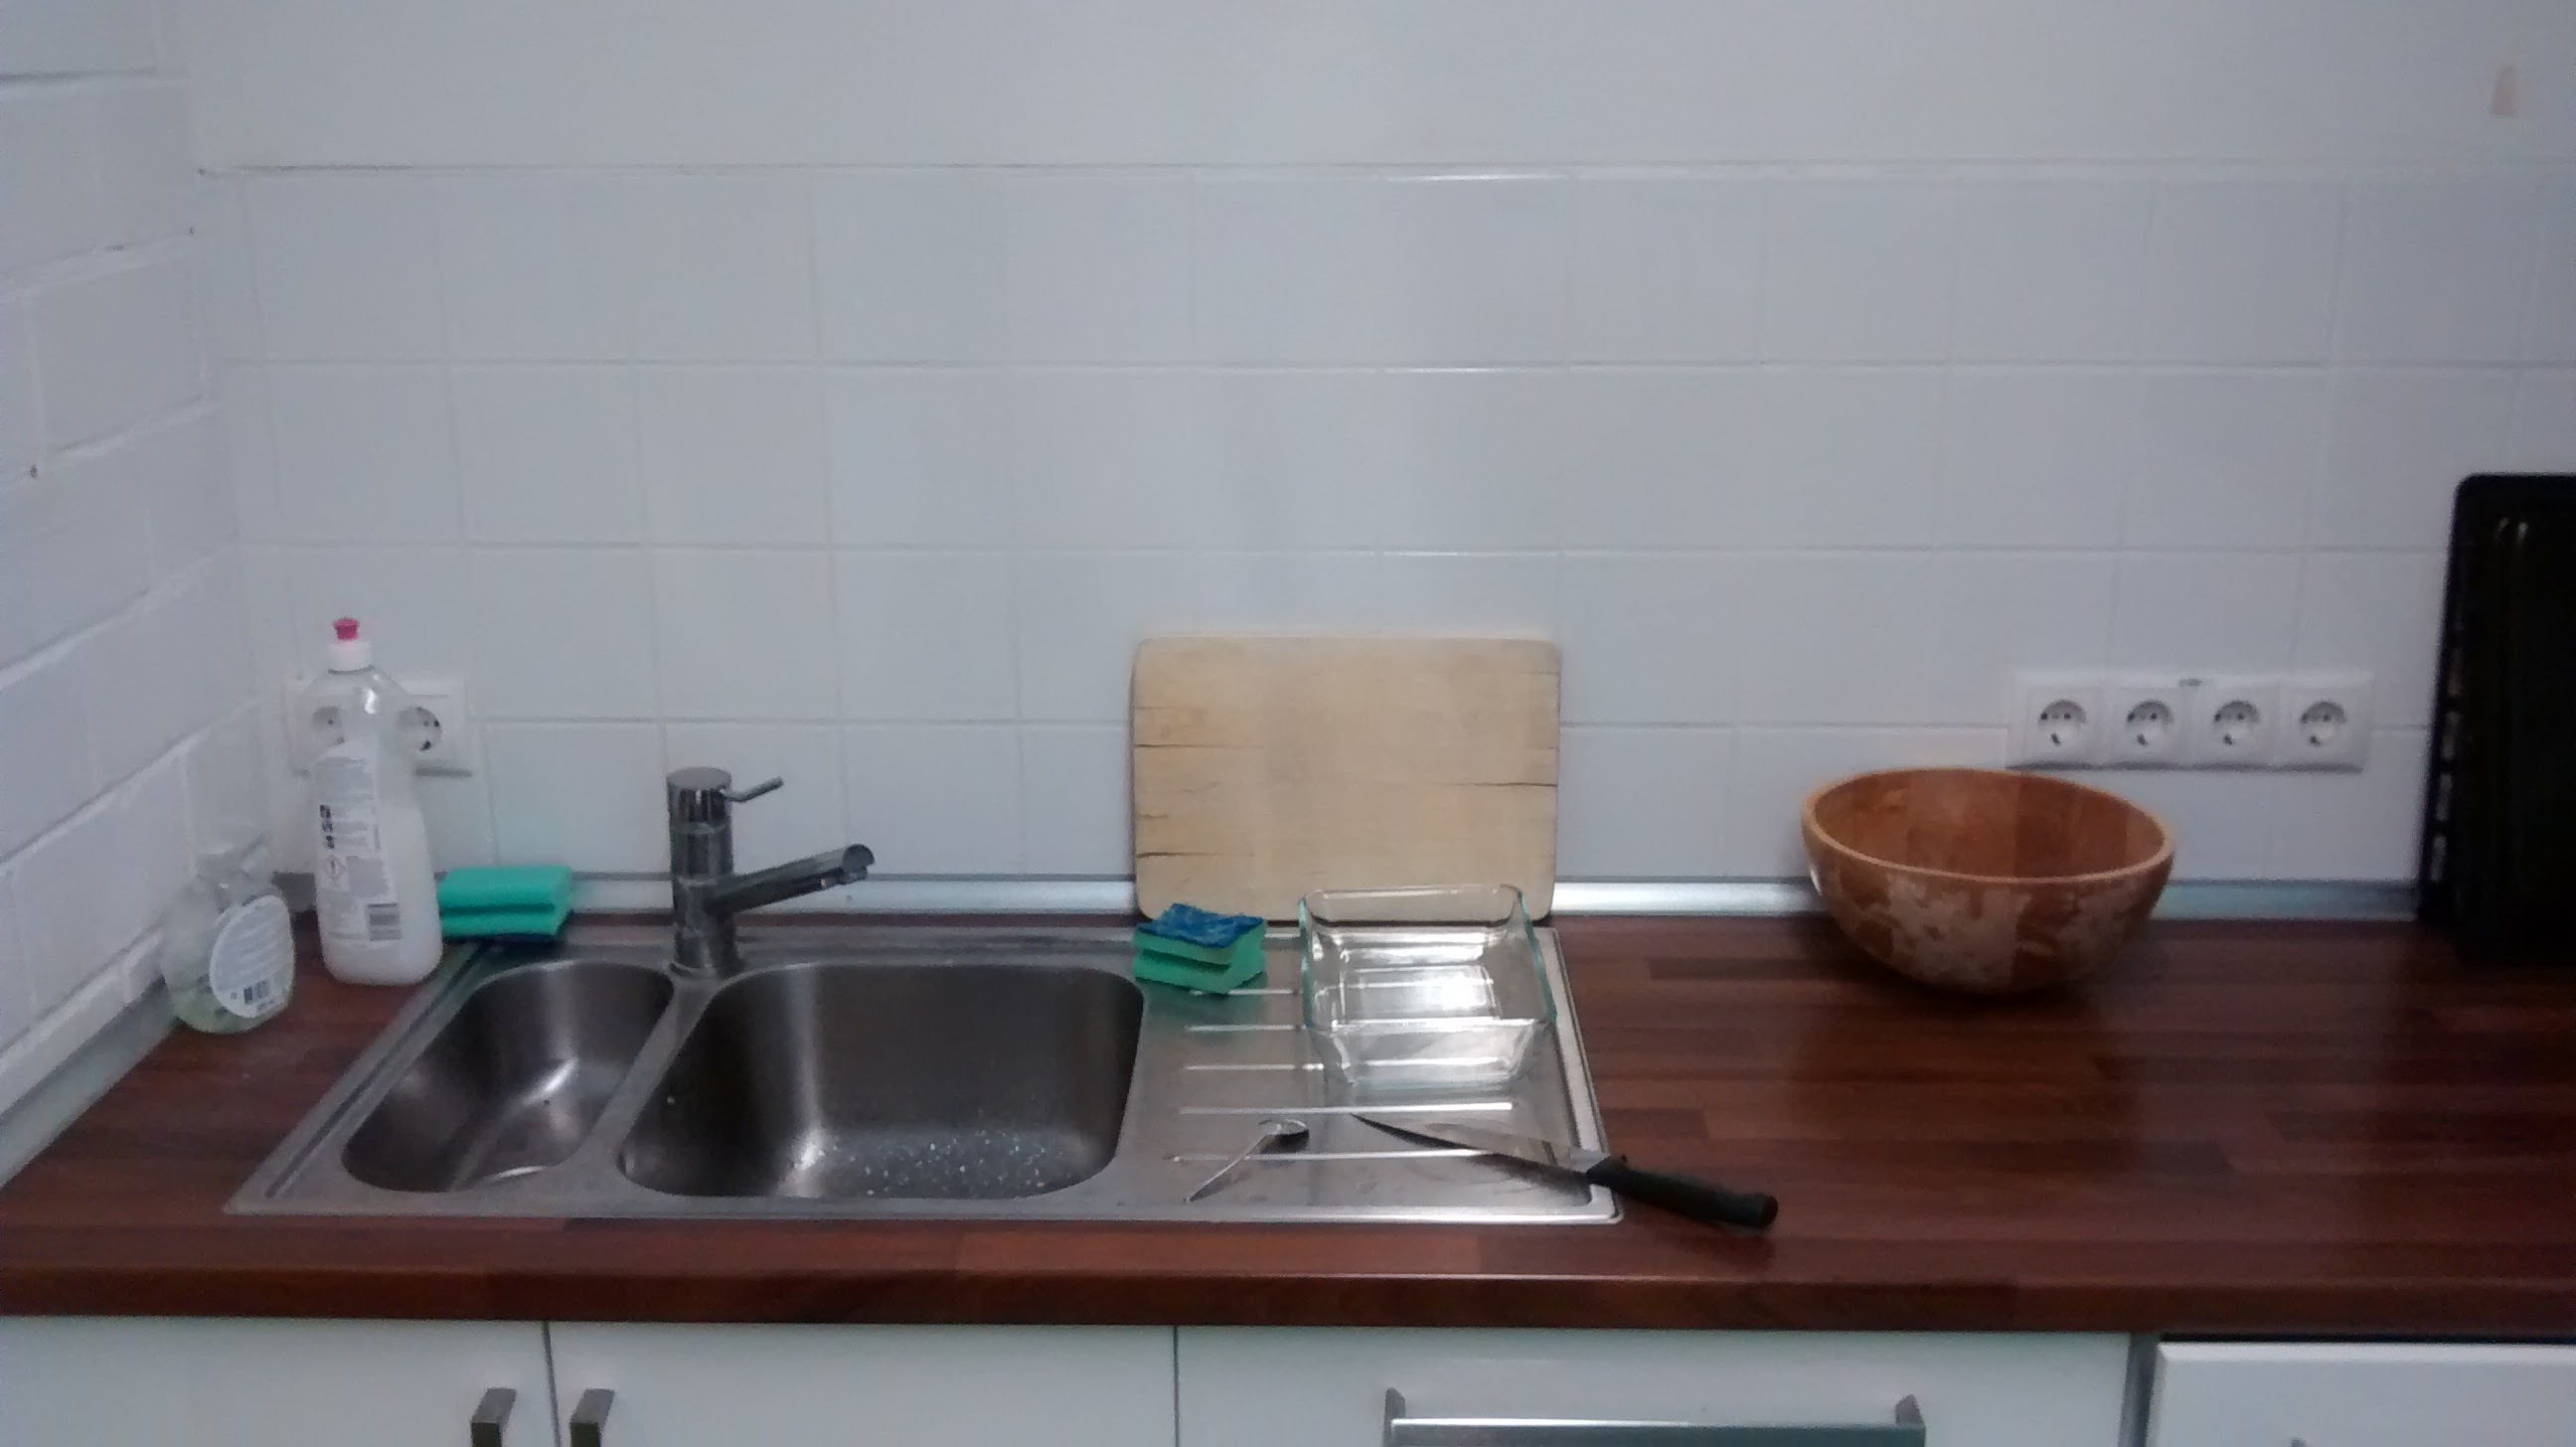
\includegraphics[width=\textwidth]{images/sink.jpg}
        \caption{Sink}
        \label{fig:sink}
    \end{subfigure}
    ~ %add desired spacing between images, e. g. ~, \quad, \qquad, \hfill etc. 
      %(or a blank line to force the subfigure onto a new line)
    \begin{subfigure}[b]{0.3\textwidth}
        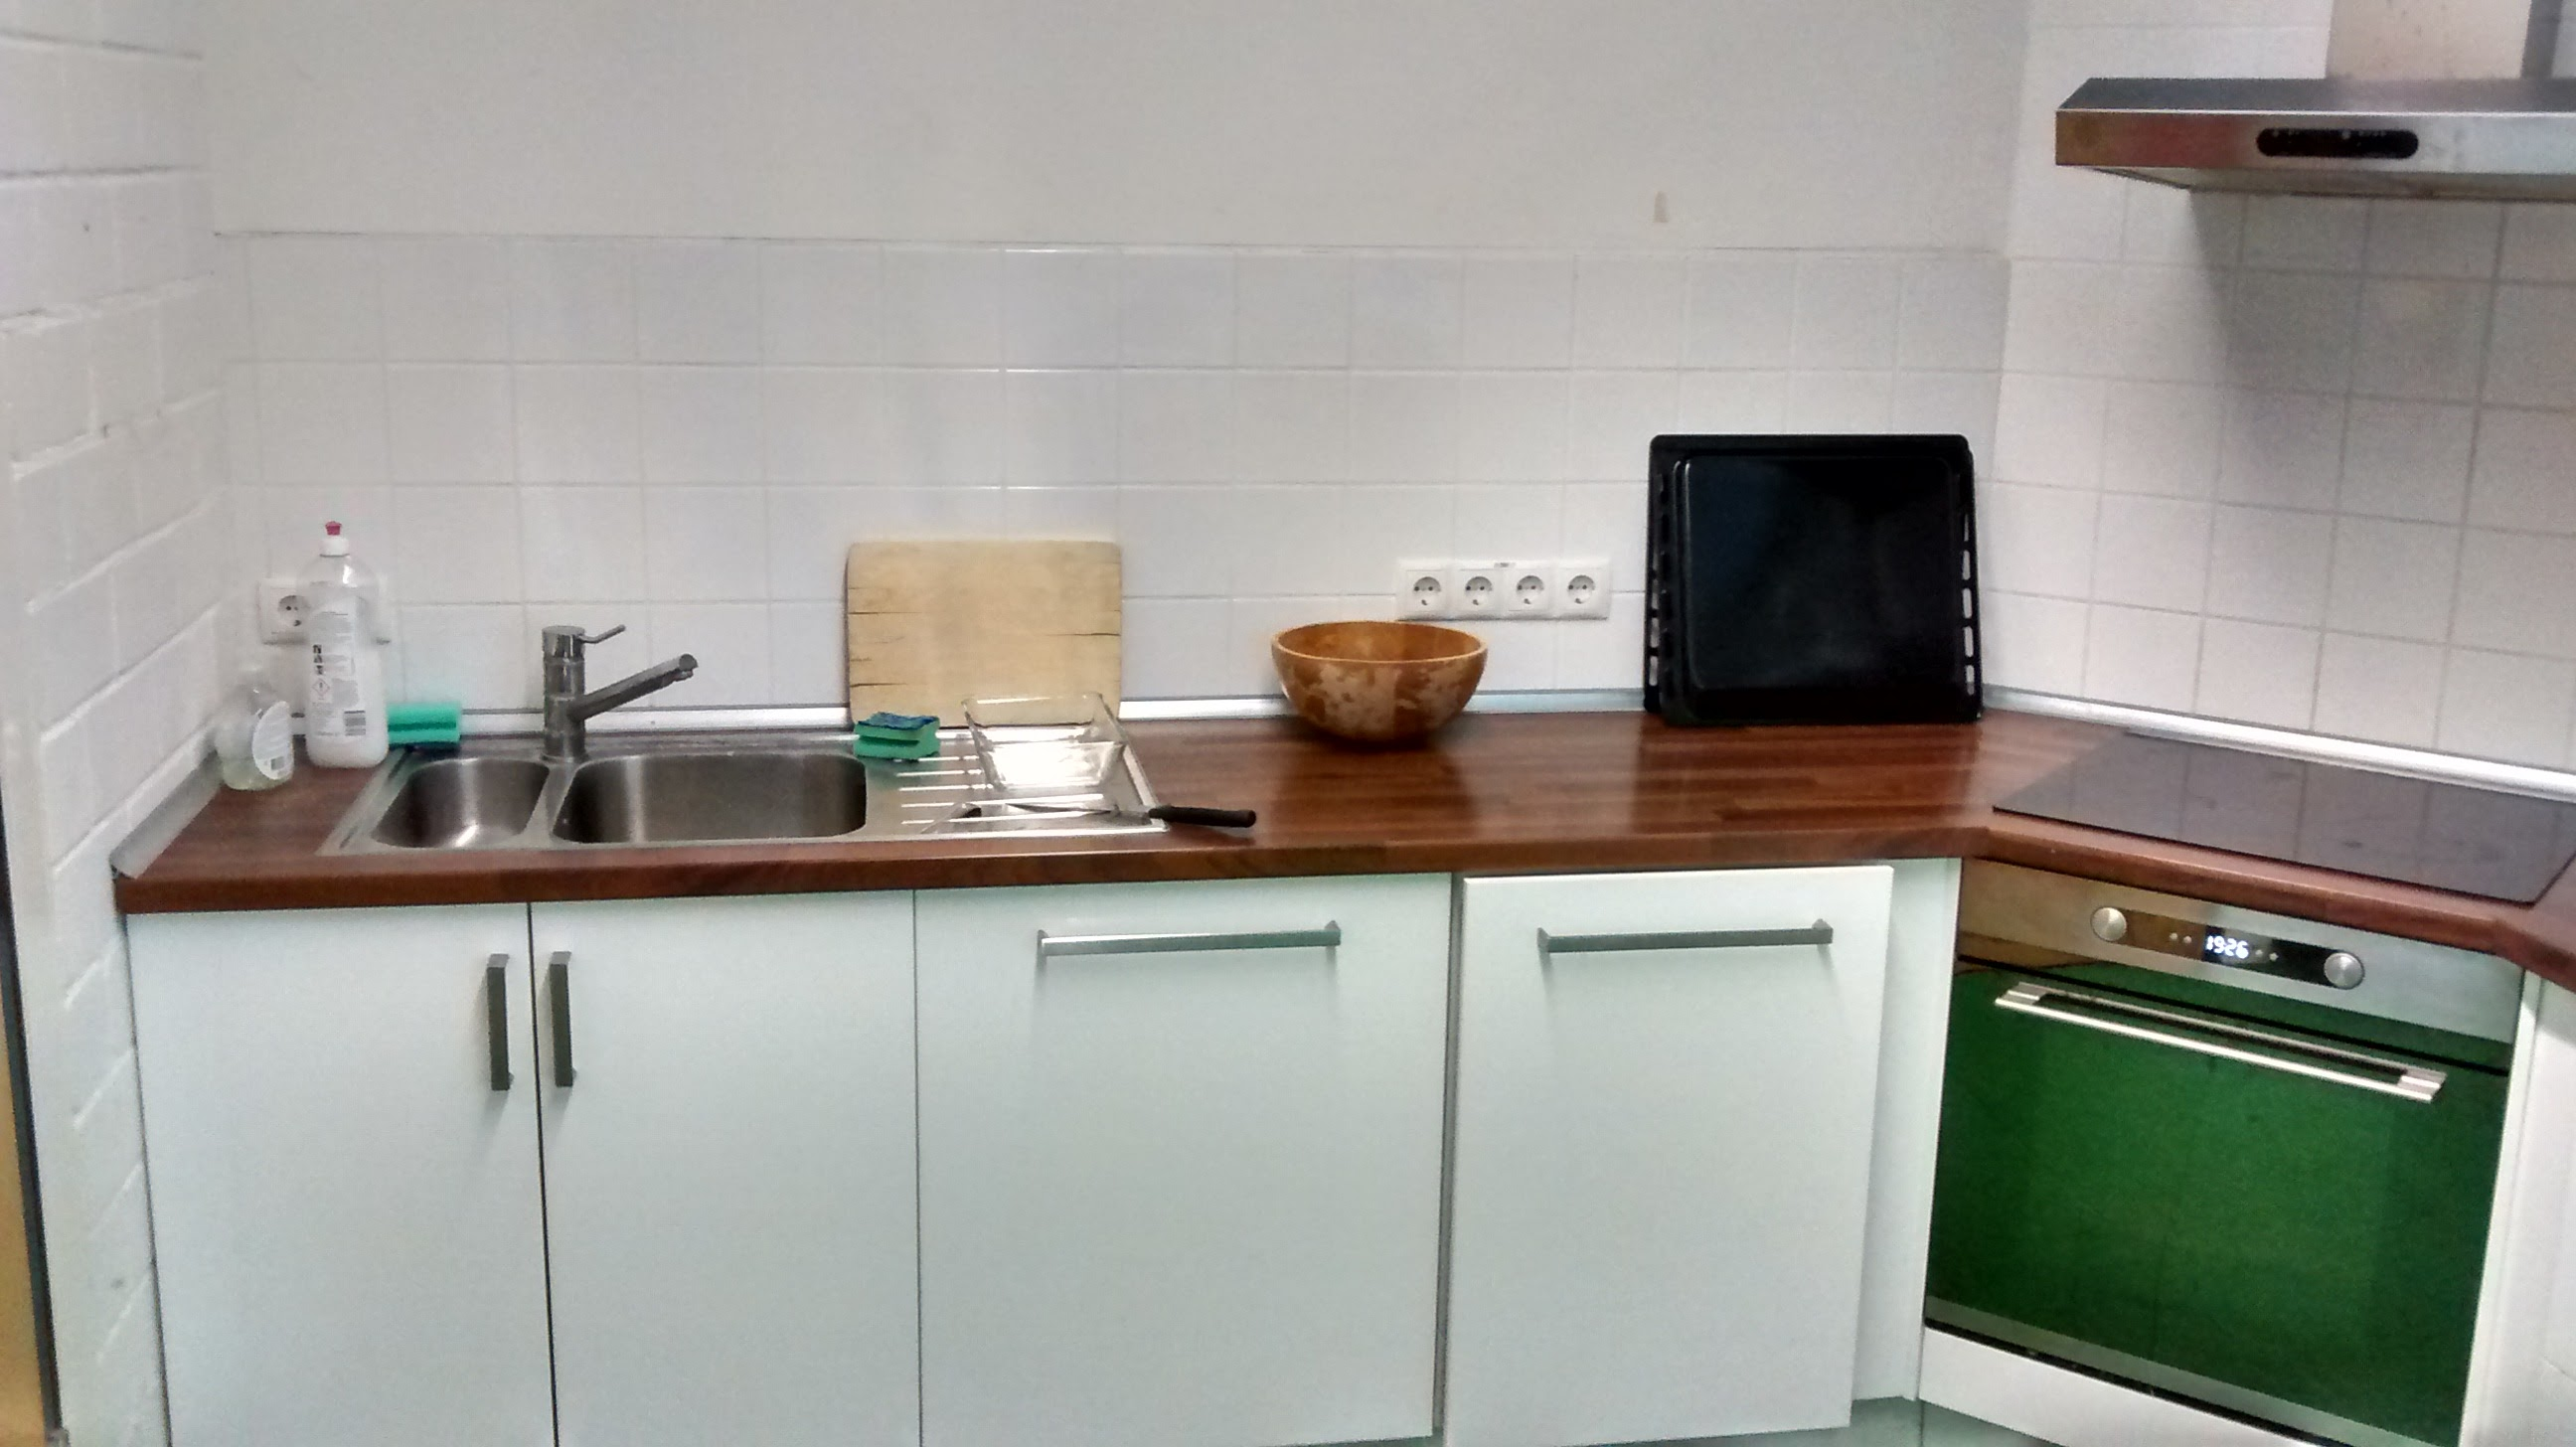
\includegraphics[width=\textwidth]{images/stove.jpg}
        \caption{Stove}
        \label{fig:stove}
    \end{subfigure}
    ~ %add desired spacing between images, e. g. ~, \quad, \qquad, \hfill etc. 
    %(or a blank line to force the subfigure onto a new line)
    \begin{subfigure}[b]{0.3\textwidth}
        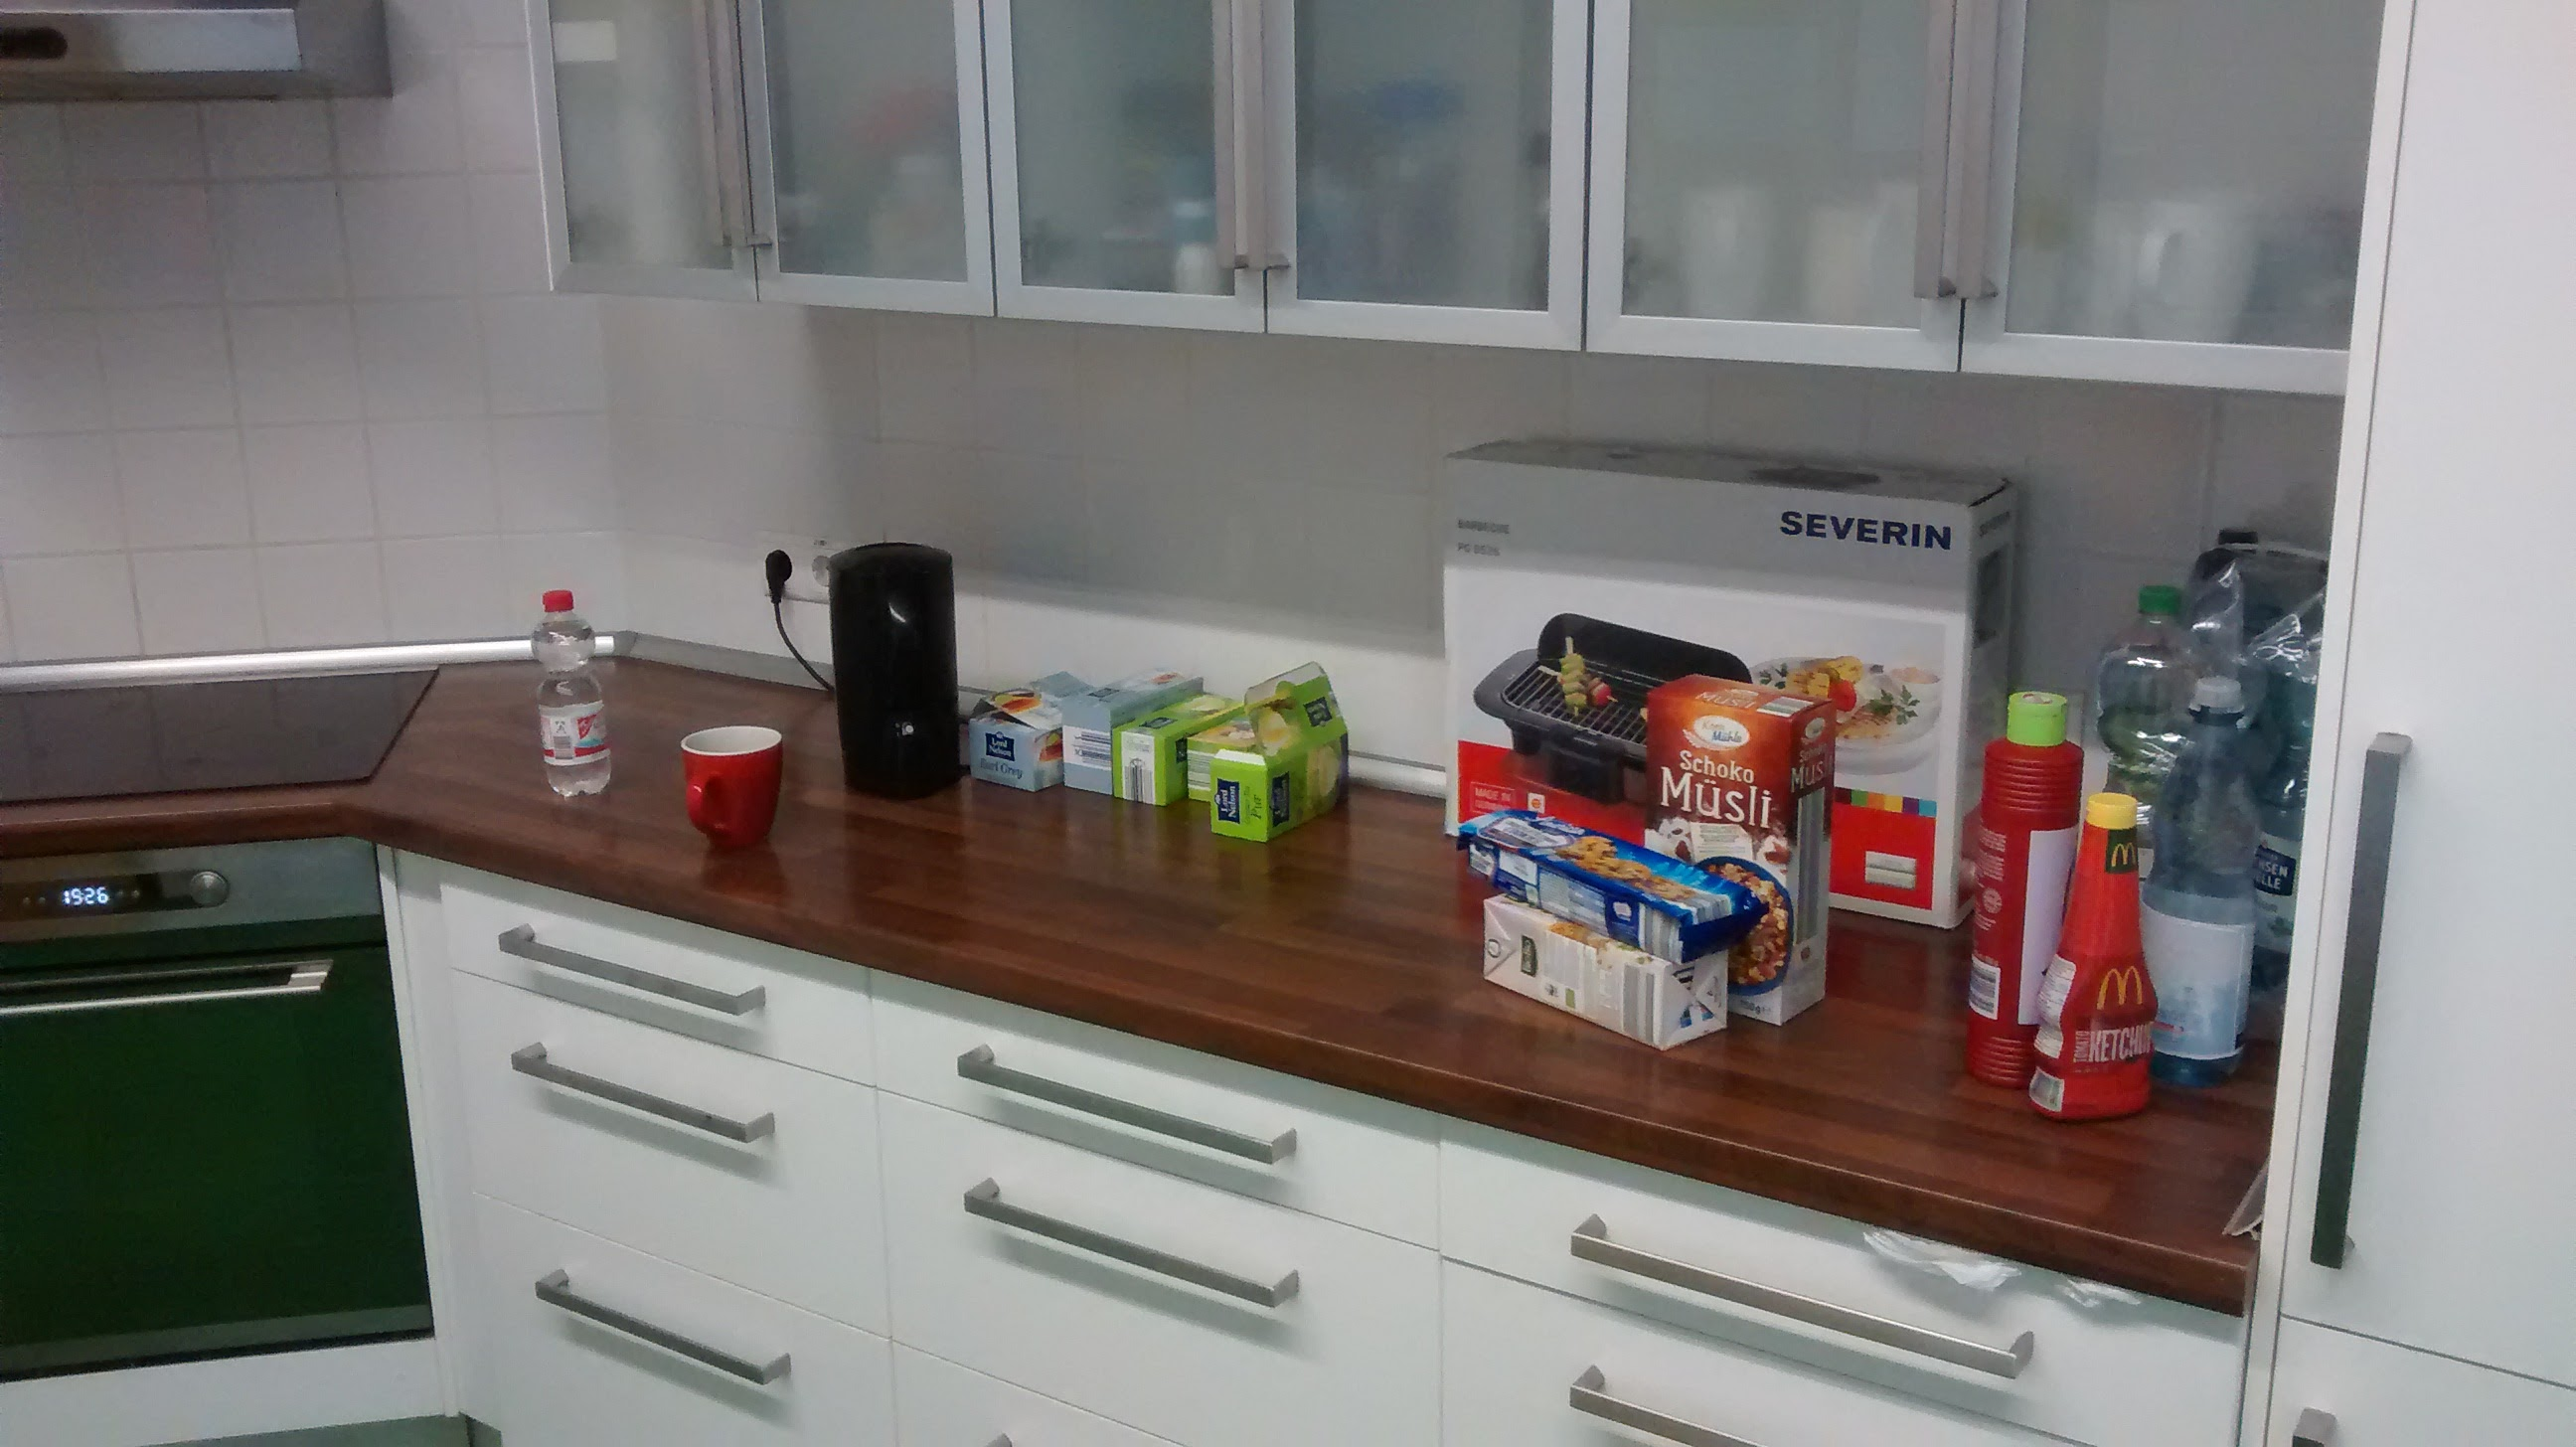
\includegraphics[width=\textwidth]{images/counter-top.jpg}
        \caption{counter-top}
        \label{fig:counter-top}
    \end{subfigure}
    \caption{Different possible object locations}\label{fig:alllocations}
\end{figure}
\begin{figure}
    \centering
    \begin{subfigure}[b]{0.3\textwidth}
        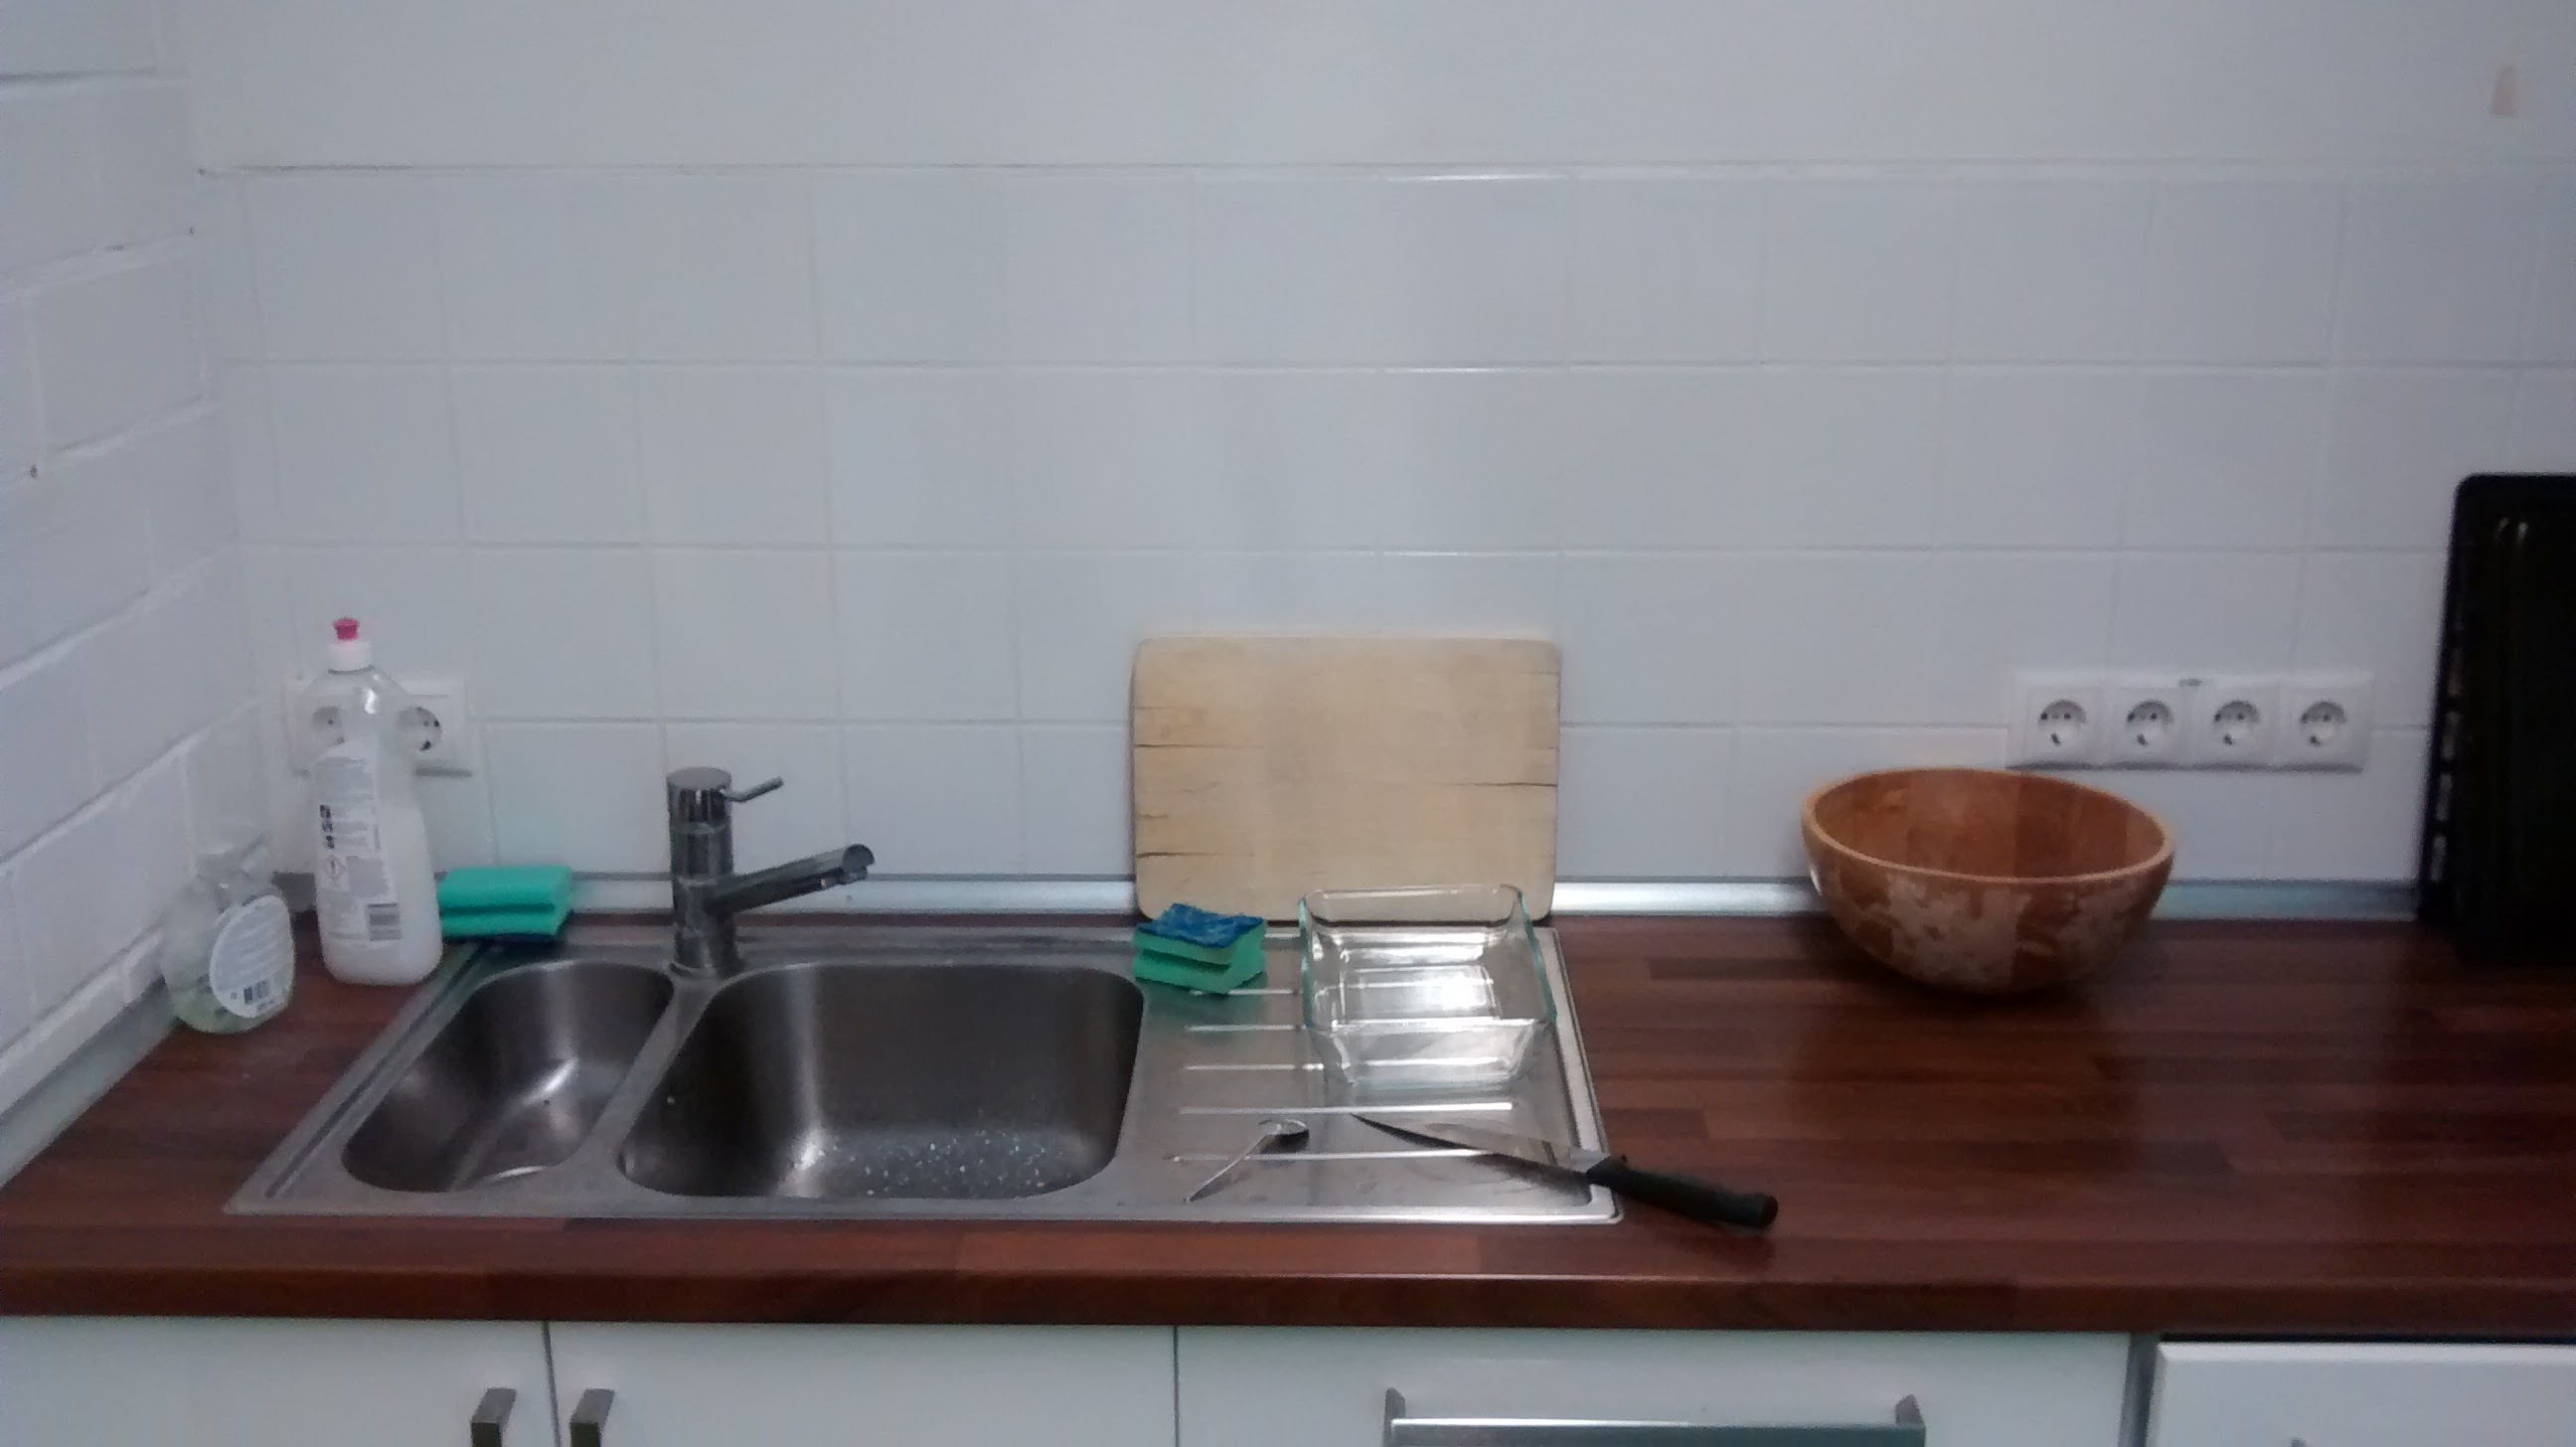
\includegraphics[width=\textwidth]{images/sink.jpg}
        \caption{Sink}
        \label{fig:sink}
    \end{subfigure}
    ~ %add desired spacing between images, e. g. ~, \quad, \qquad, \hfill etc. 
      %(or a blank line to force the subfigure onto a new line)
    \begin{subfigure}[b]{0.3\textwidth}
        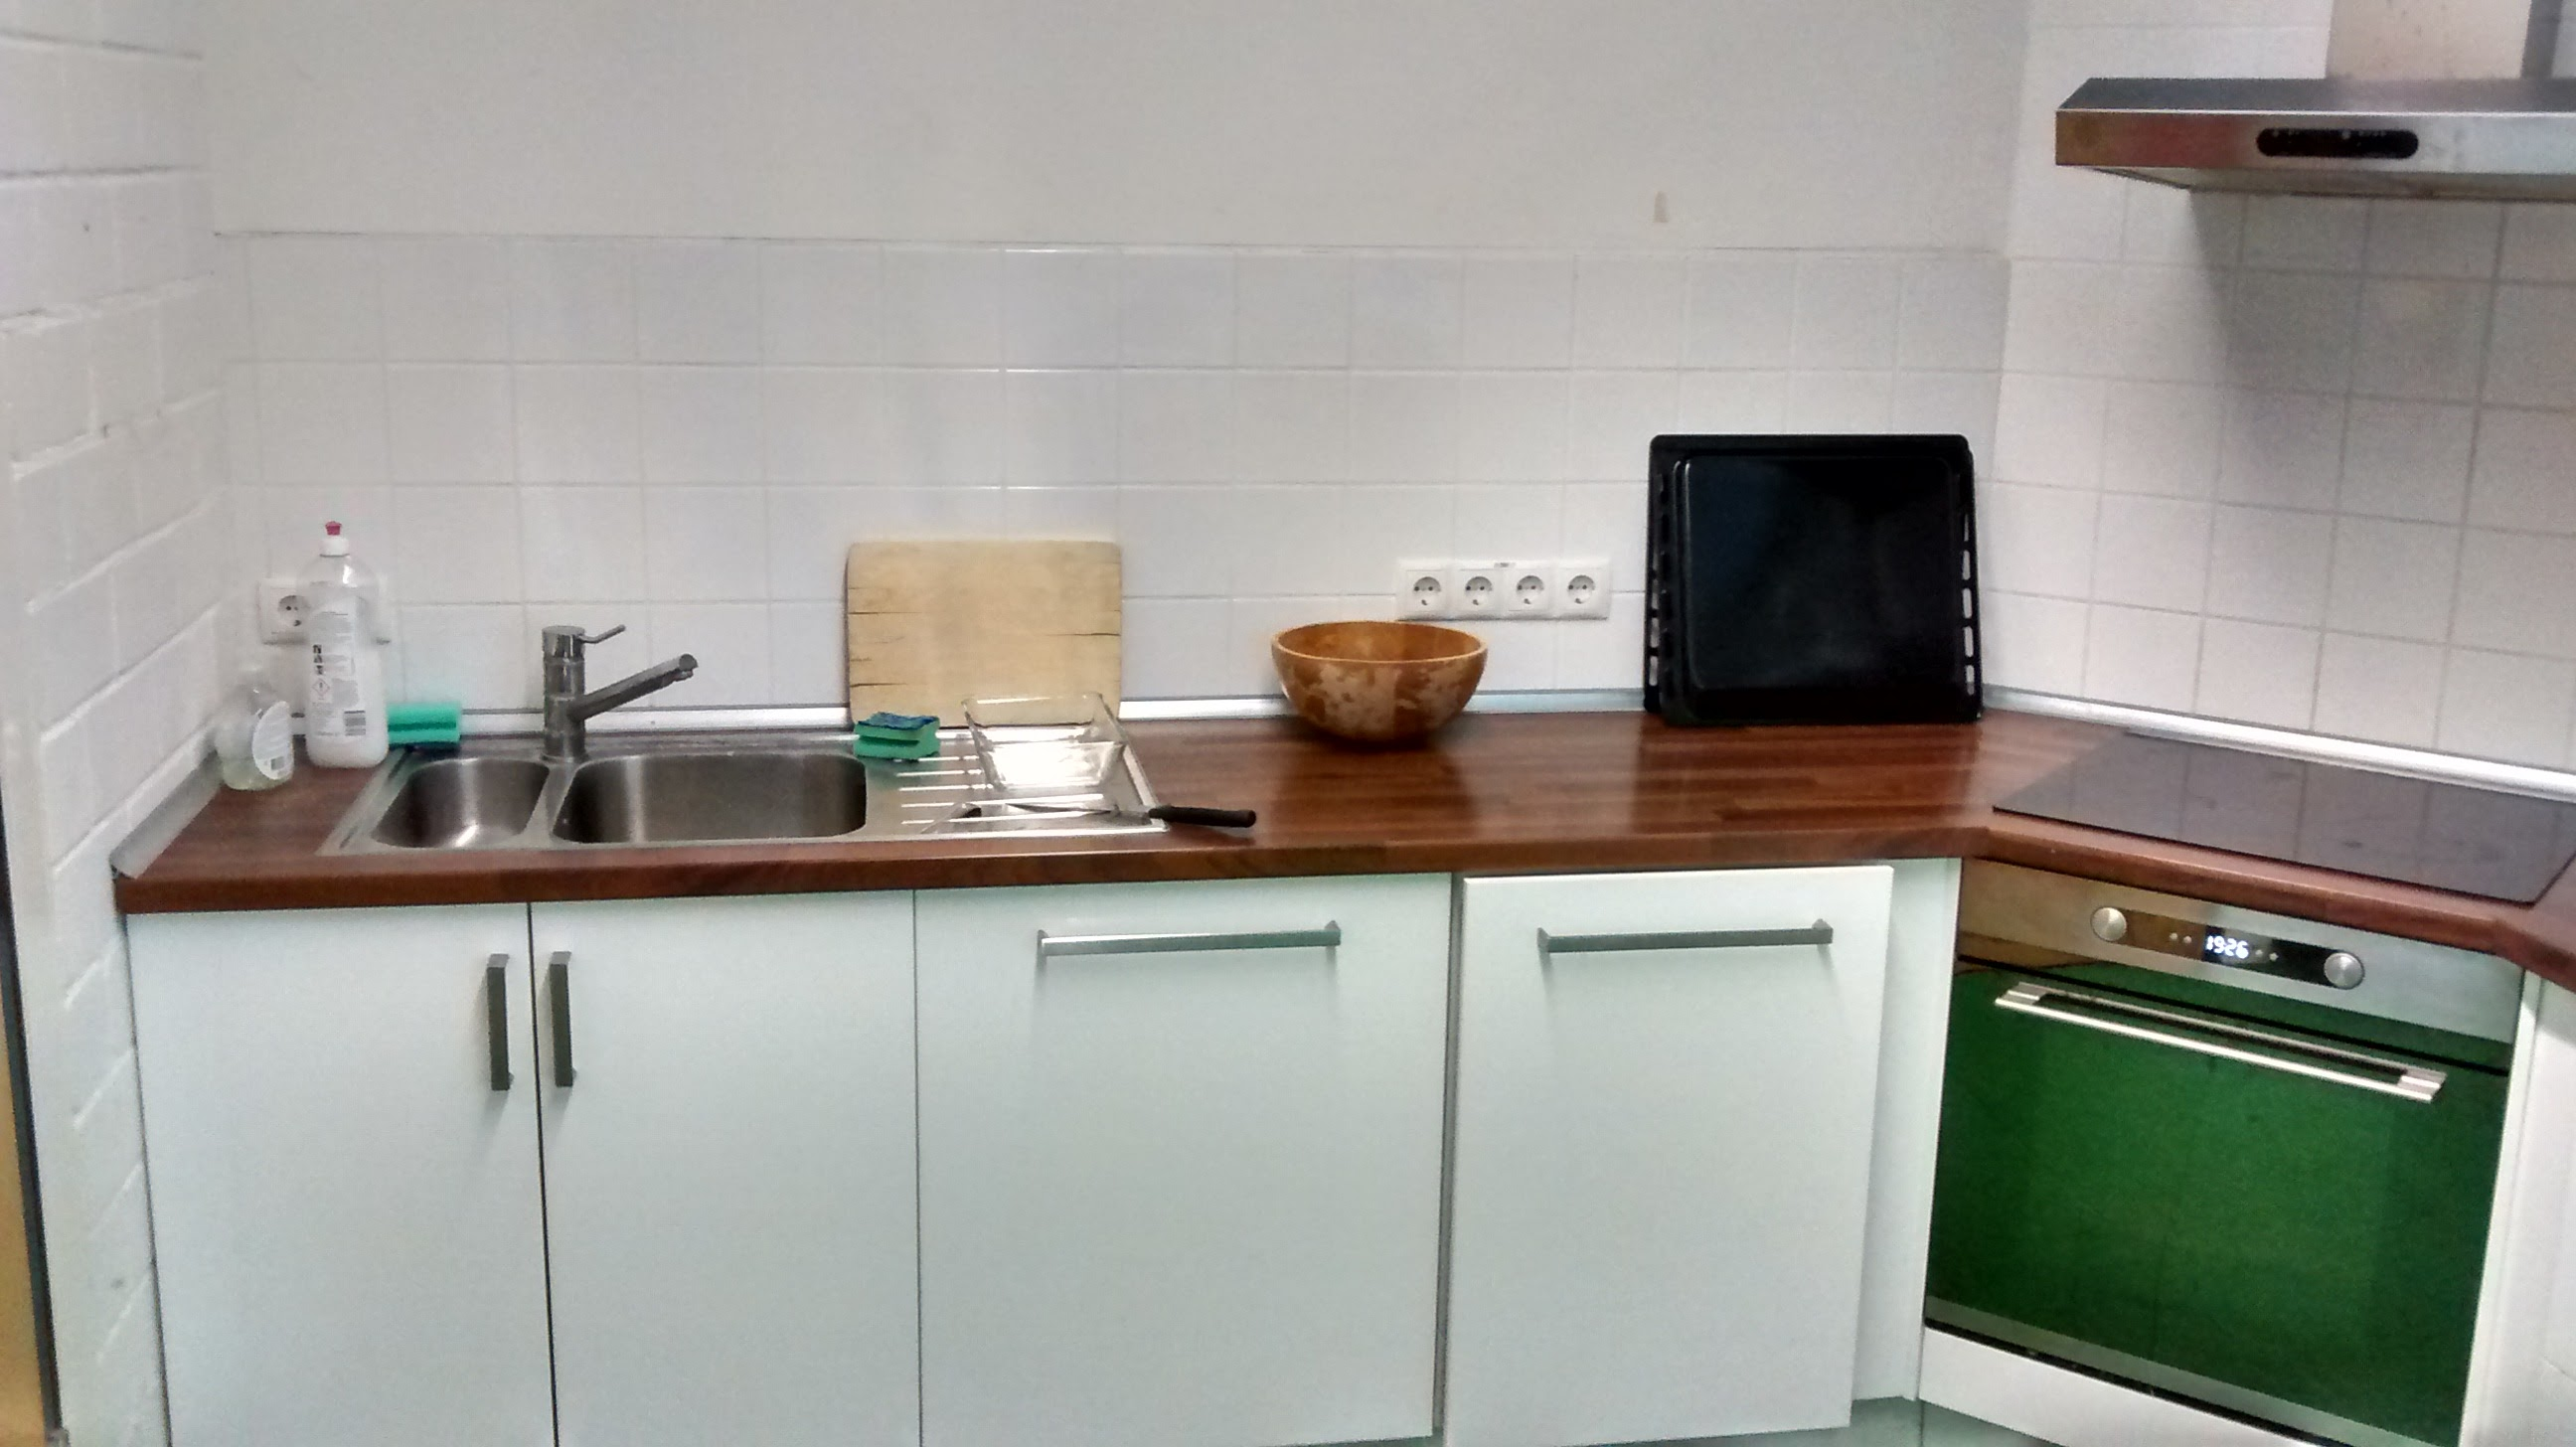
\includegraphics[width=\textwidth]{images/stove.jpg}
        \caption{Stove}
        \label{fig:stove}
    \end{subfigure}
    ~ %add desired spacing between images, e. g. ~, \quad, \qquad, \hfill etc. 
    %(or a blank line to force the subfigure onto a new line)
    \begin{subfigure}[b]{0.3\textwidth}
        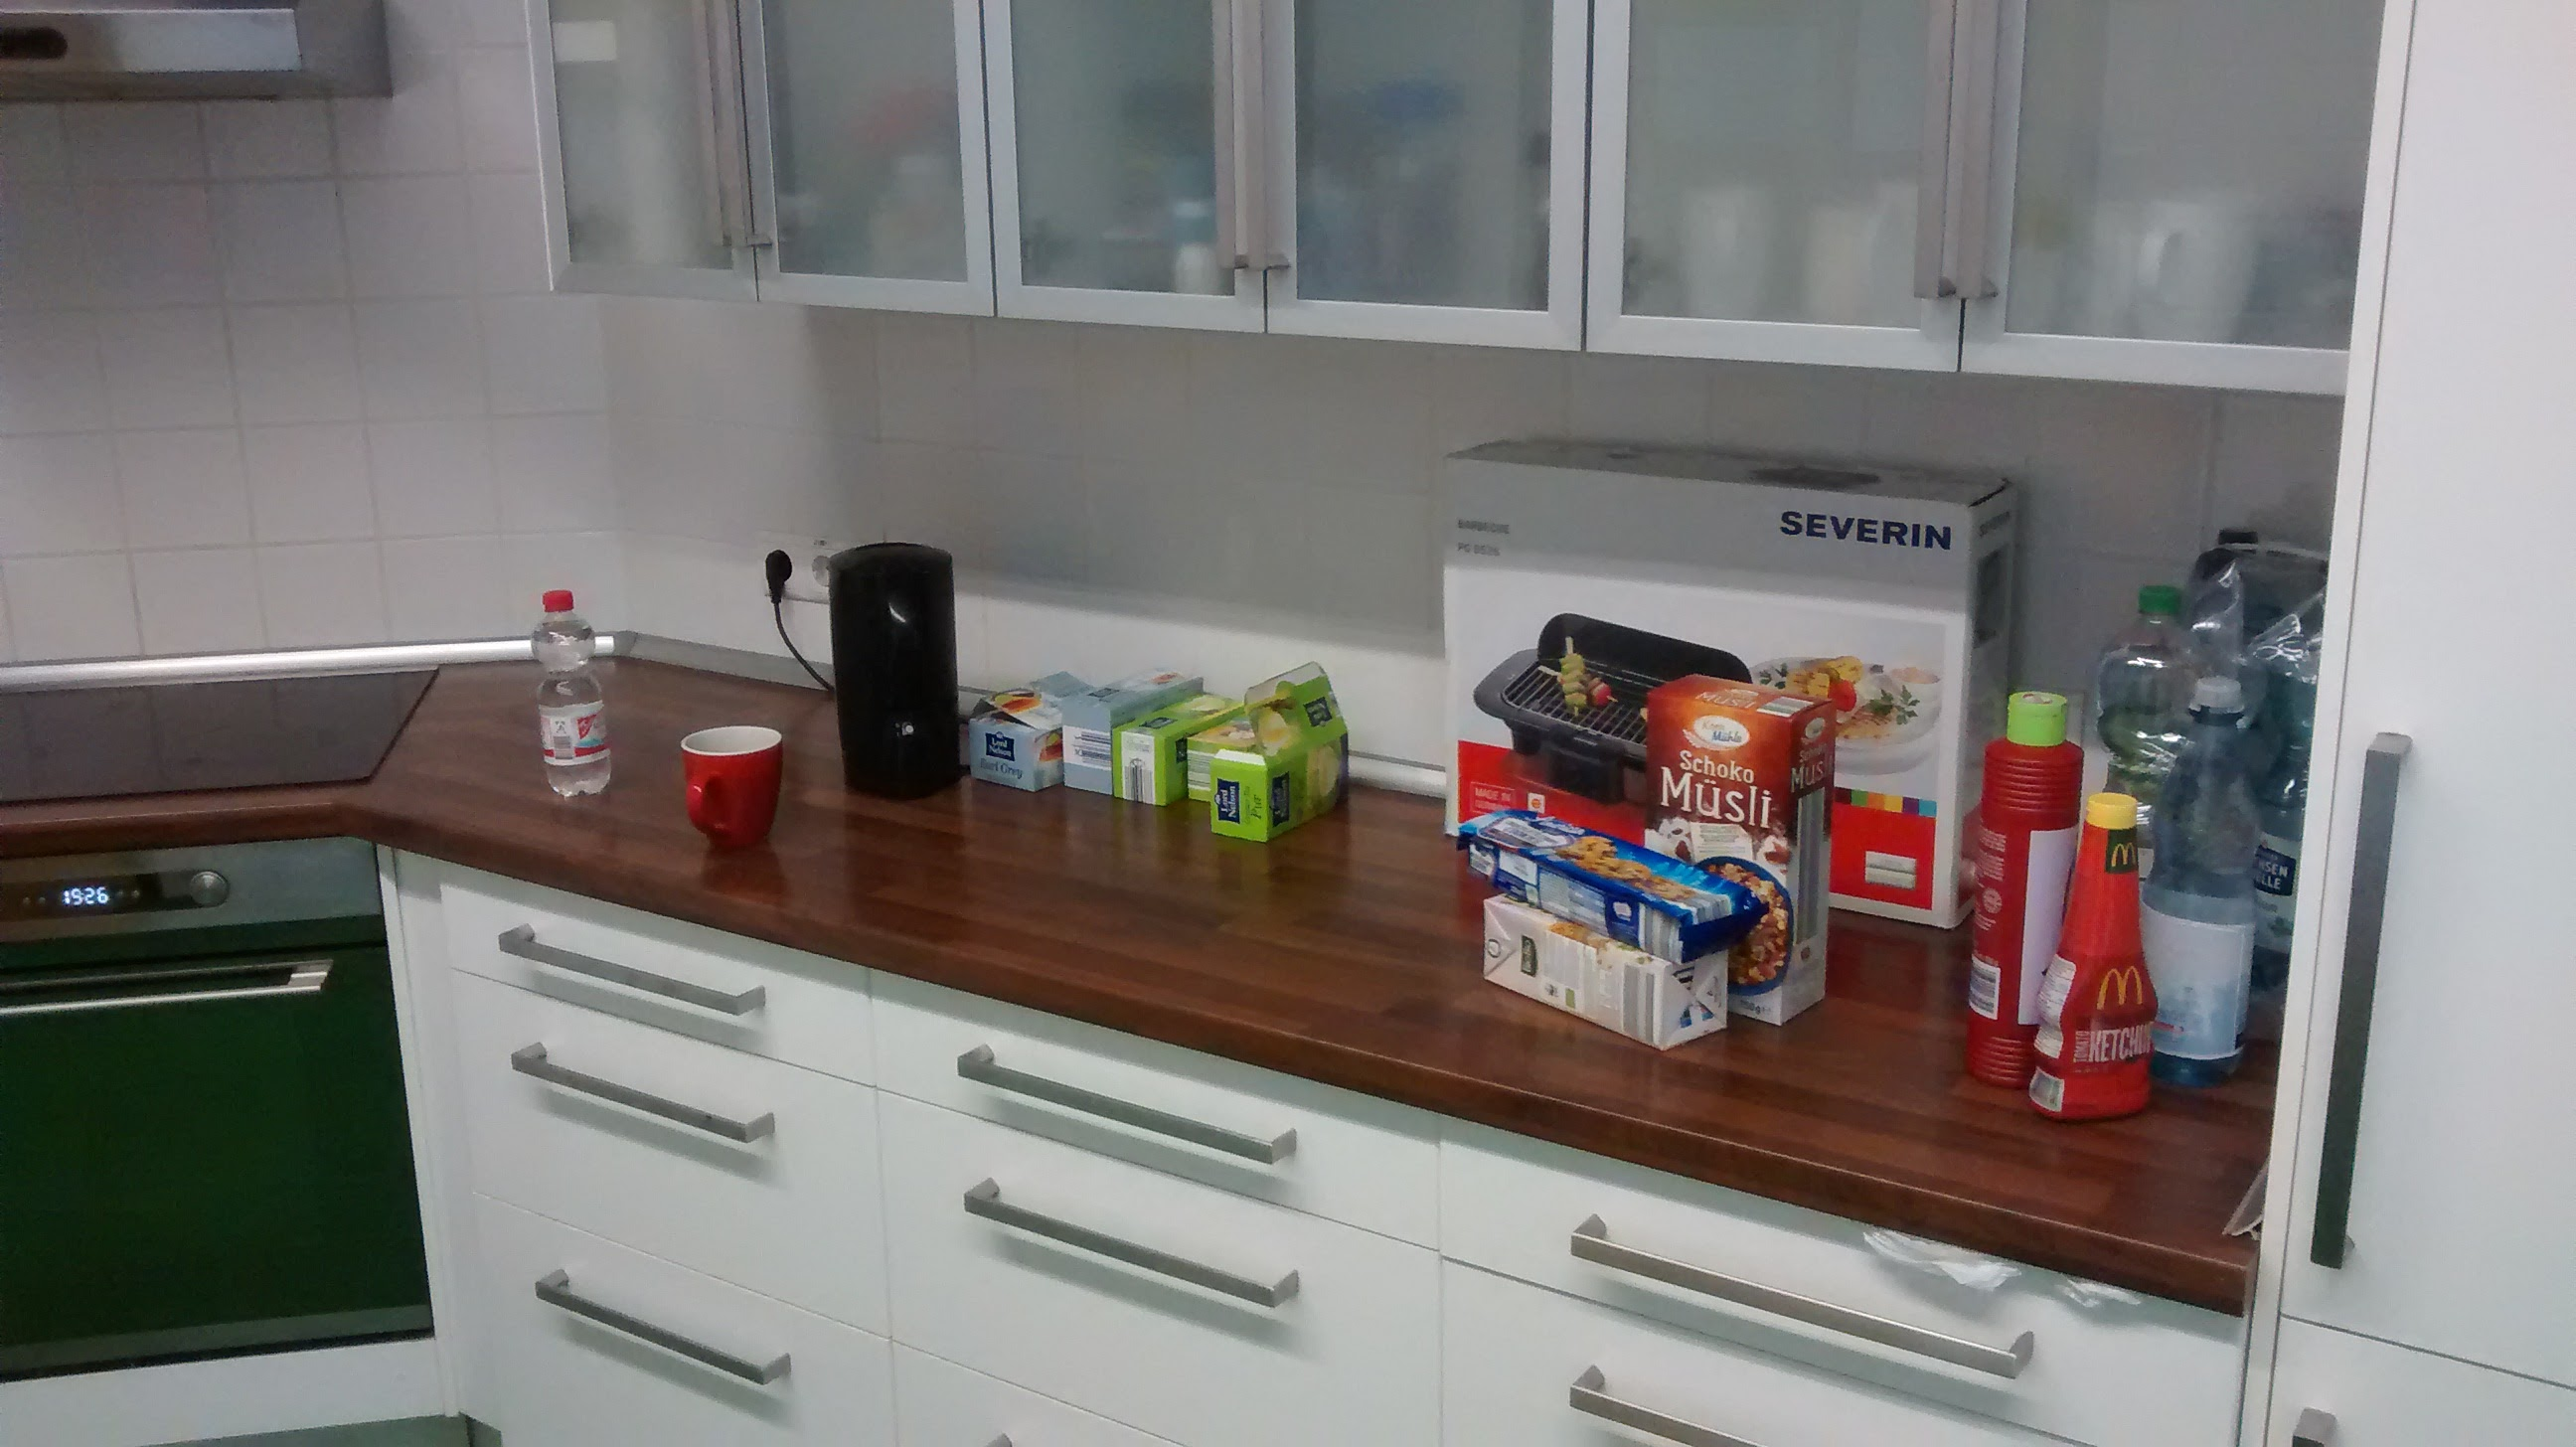
\includegraphics[width=\textwidth]{images/counter-top.jpg}
        \caption{counter-top}
        \label{fig:counter-top}
    \end{subfigure}
    \caption{Different possible object locations}\label{fig:alllocations}
\end{figure}
\begin{figure}
    \centering
    \begin{subfigure}[b]{0.3\textwidth}
        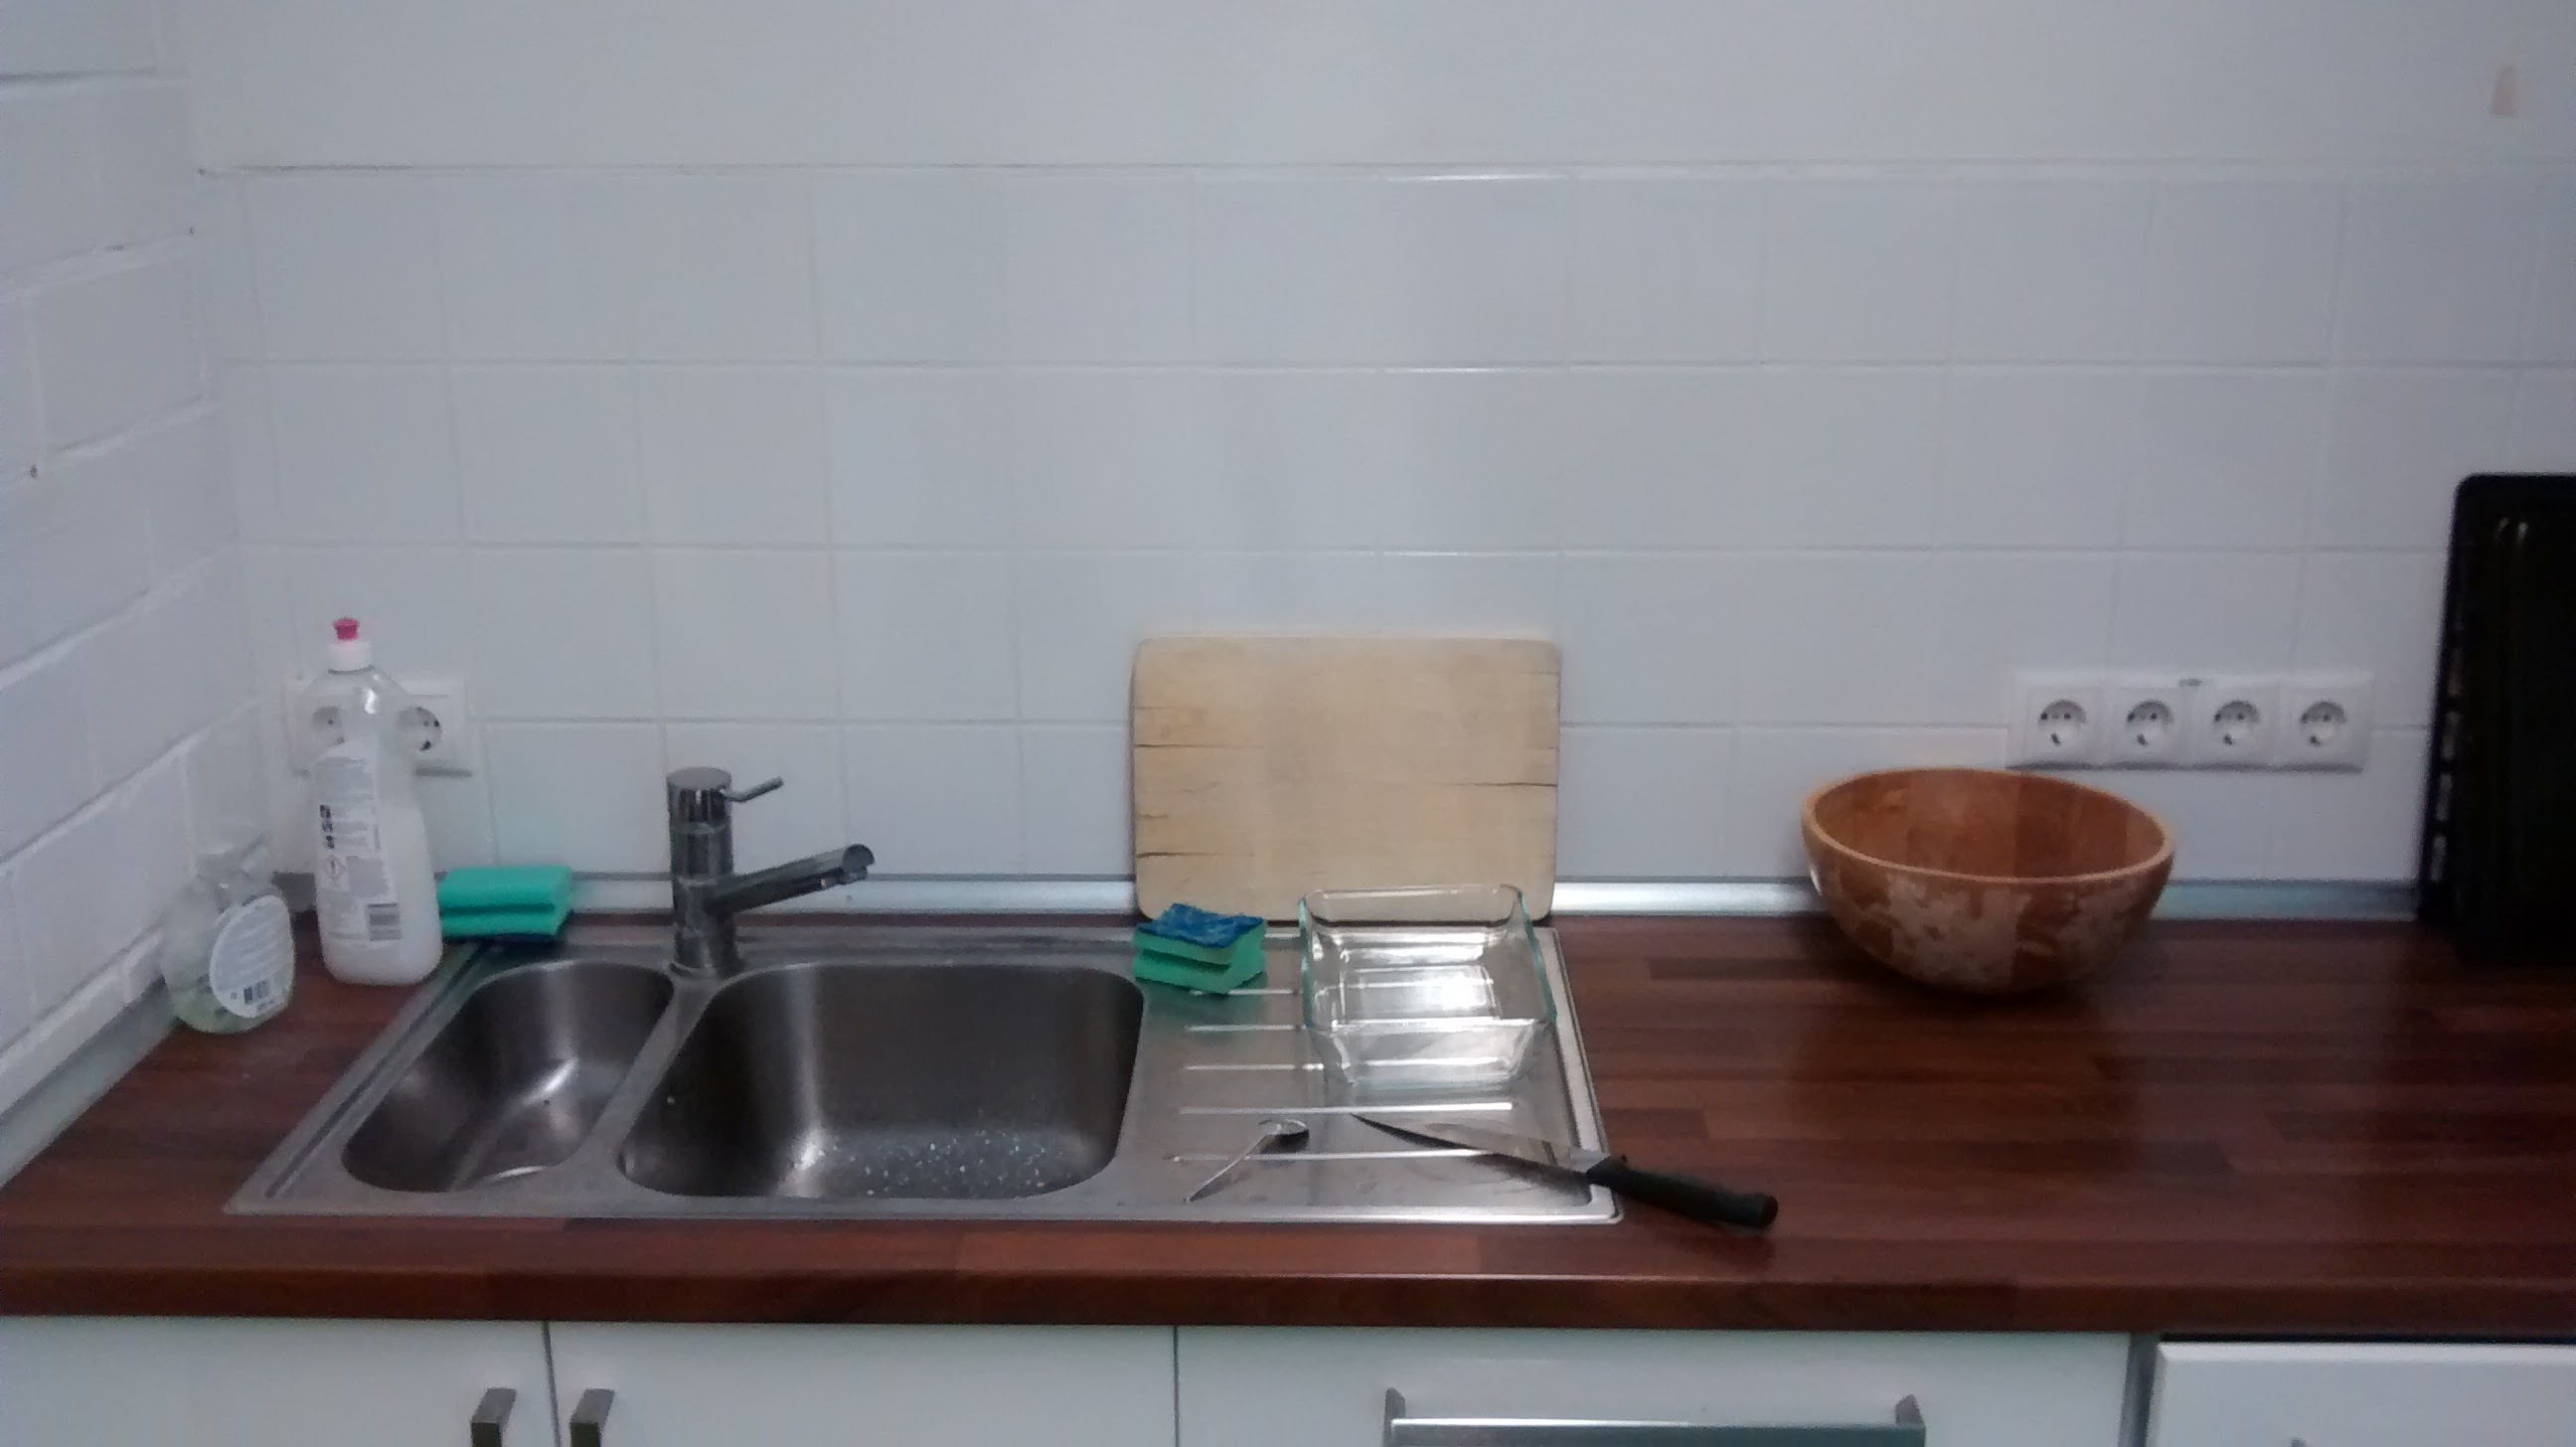
\includegraphics[width=\textwidth]{images/sink.jpg}
        \caption{Sink}
        \label{fig:sink}
    \end{subfigure}
    ~ %add desired spacing between images, e. g. ~, \quad, \qquad, \hfill etc. 
      %(or a blank line to force the subfigure onto a new line)
    \begin{subfigure}[b]{0.3\textwidth}
        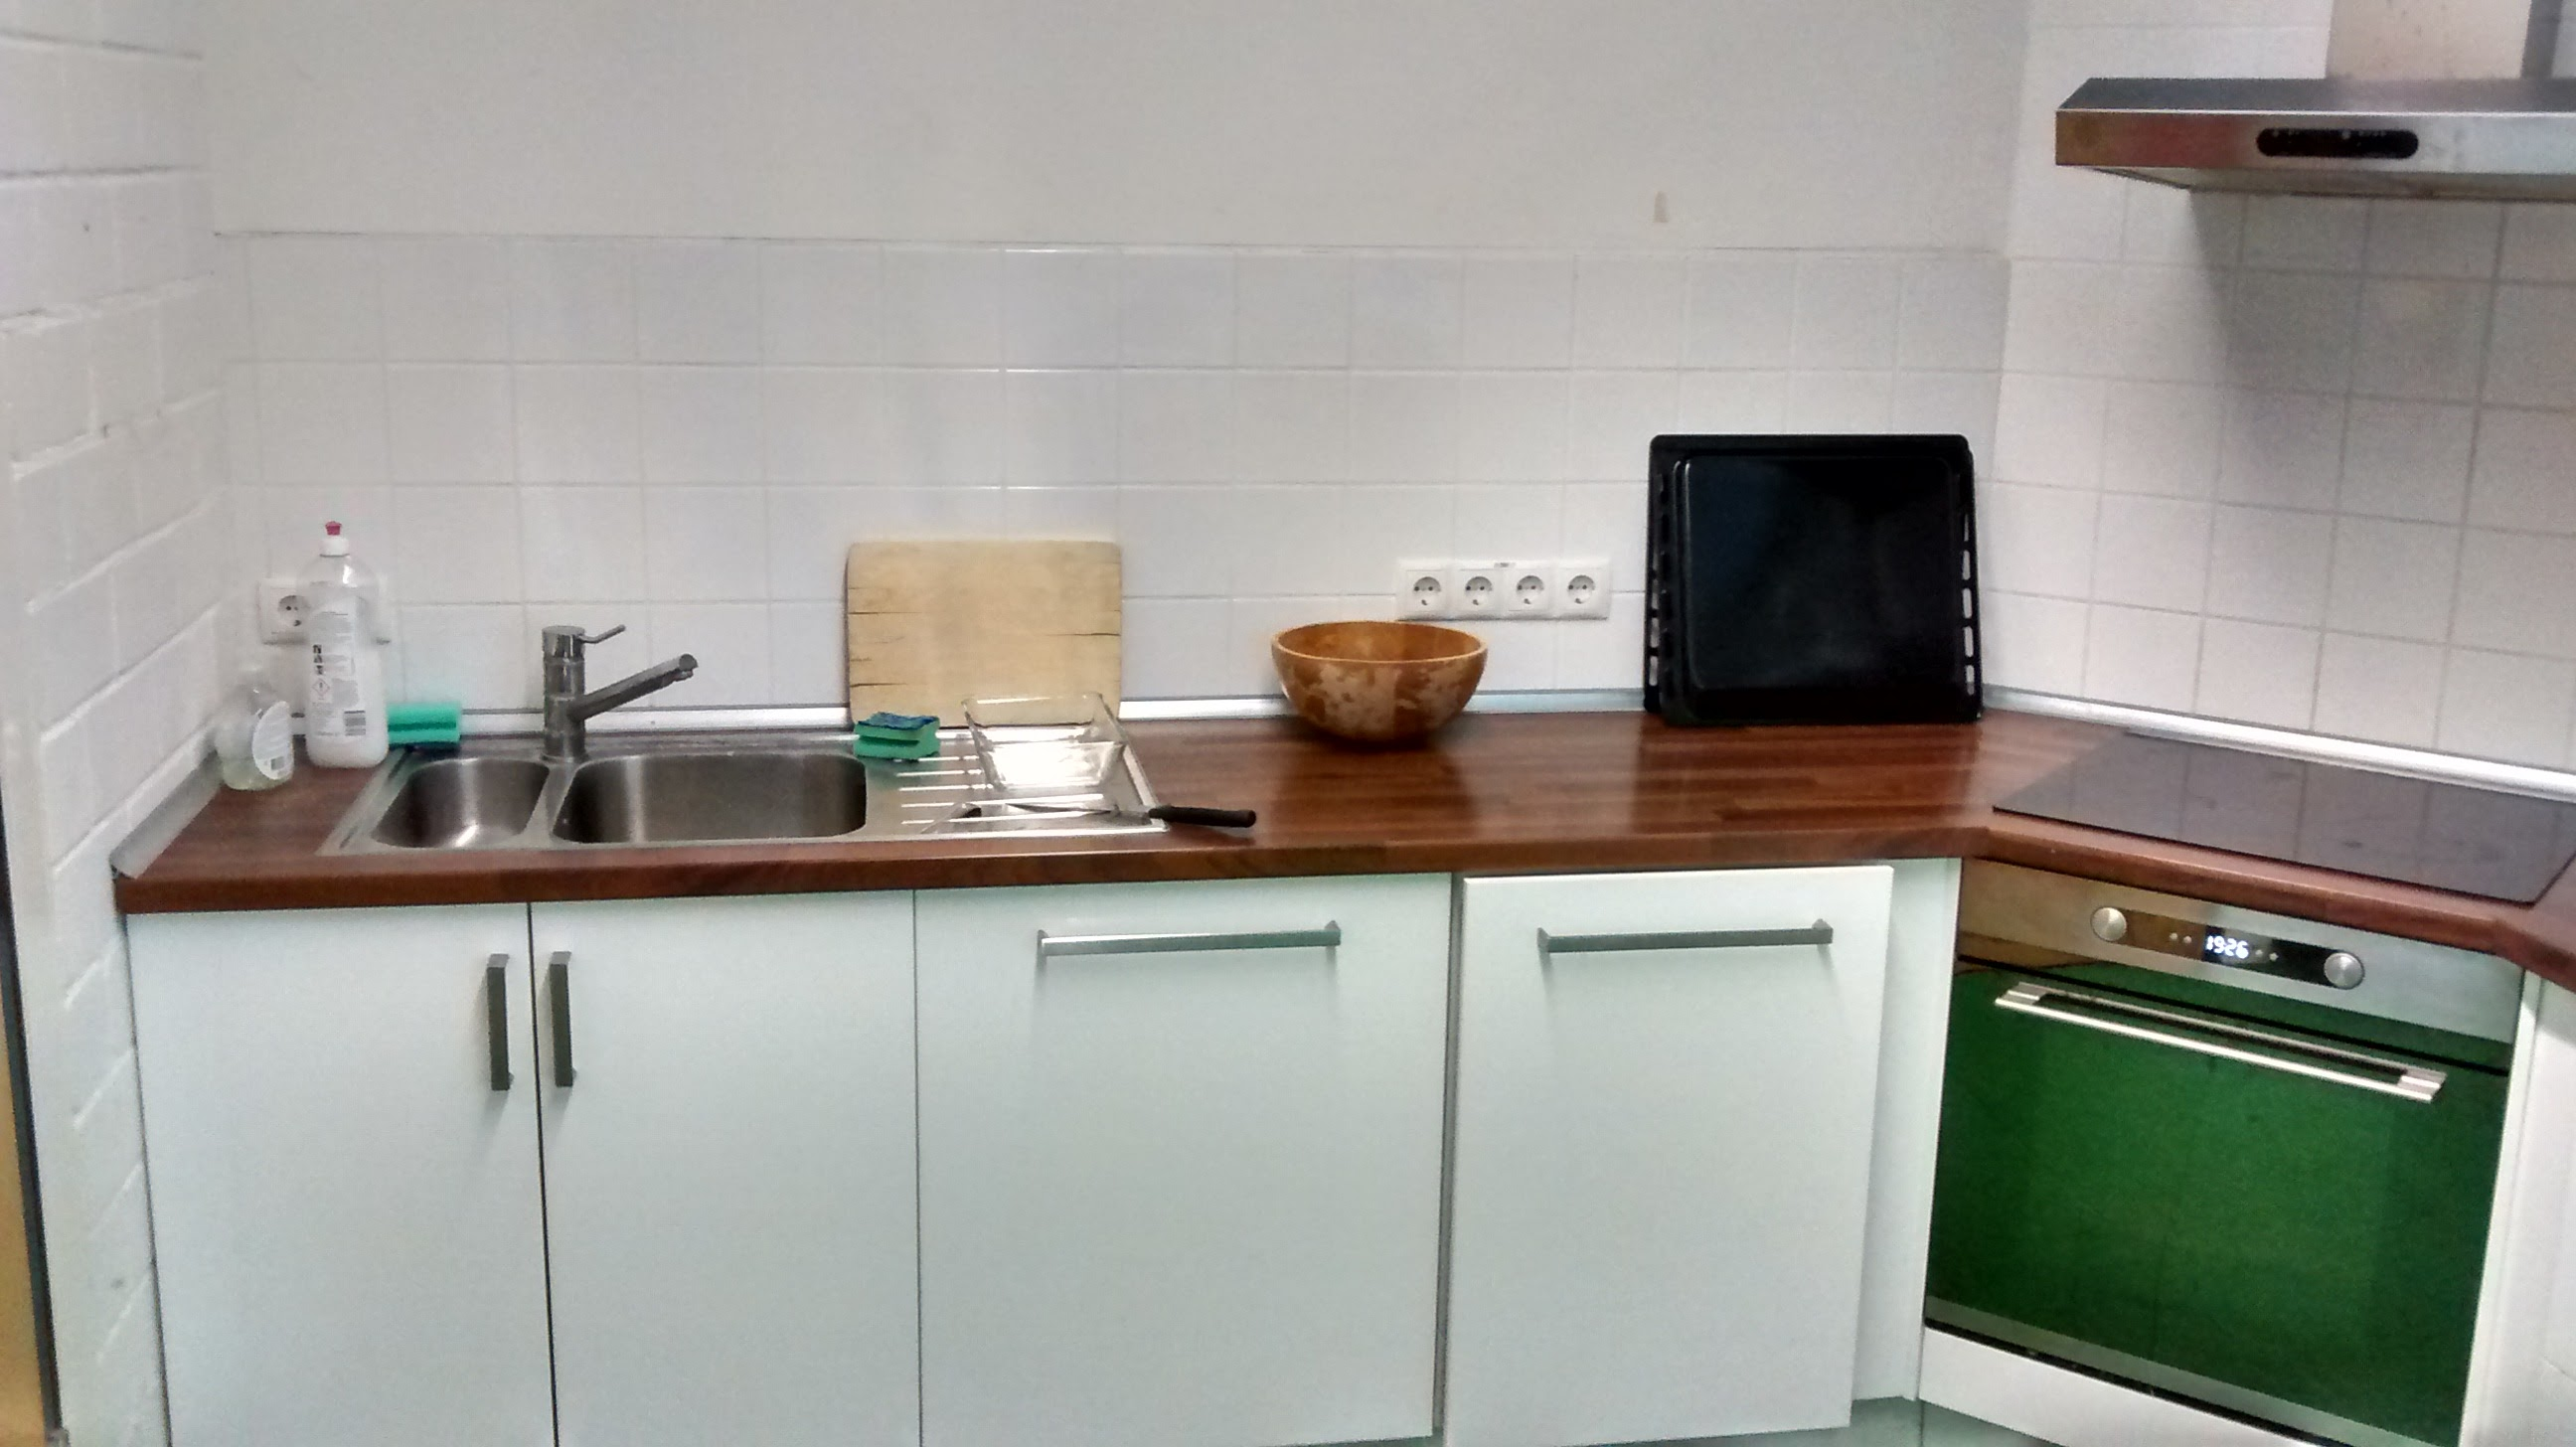
\includegraphics[width=\textwidth]{images/stove.jpg}
        \caption{Stove}
        \label{fig:stove}
    \end{subfigure}
    ~ %add desired spacing between images, e. g. ~, \quad, \qquad, \hfill etc. 
    %(or a blank line to force the subfigure onto a new line)
    \begin{subfigure}[b]{0.3\textwidth}
        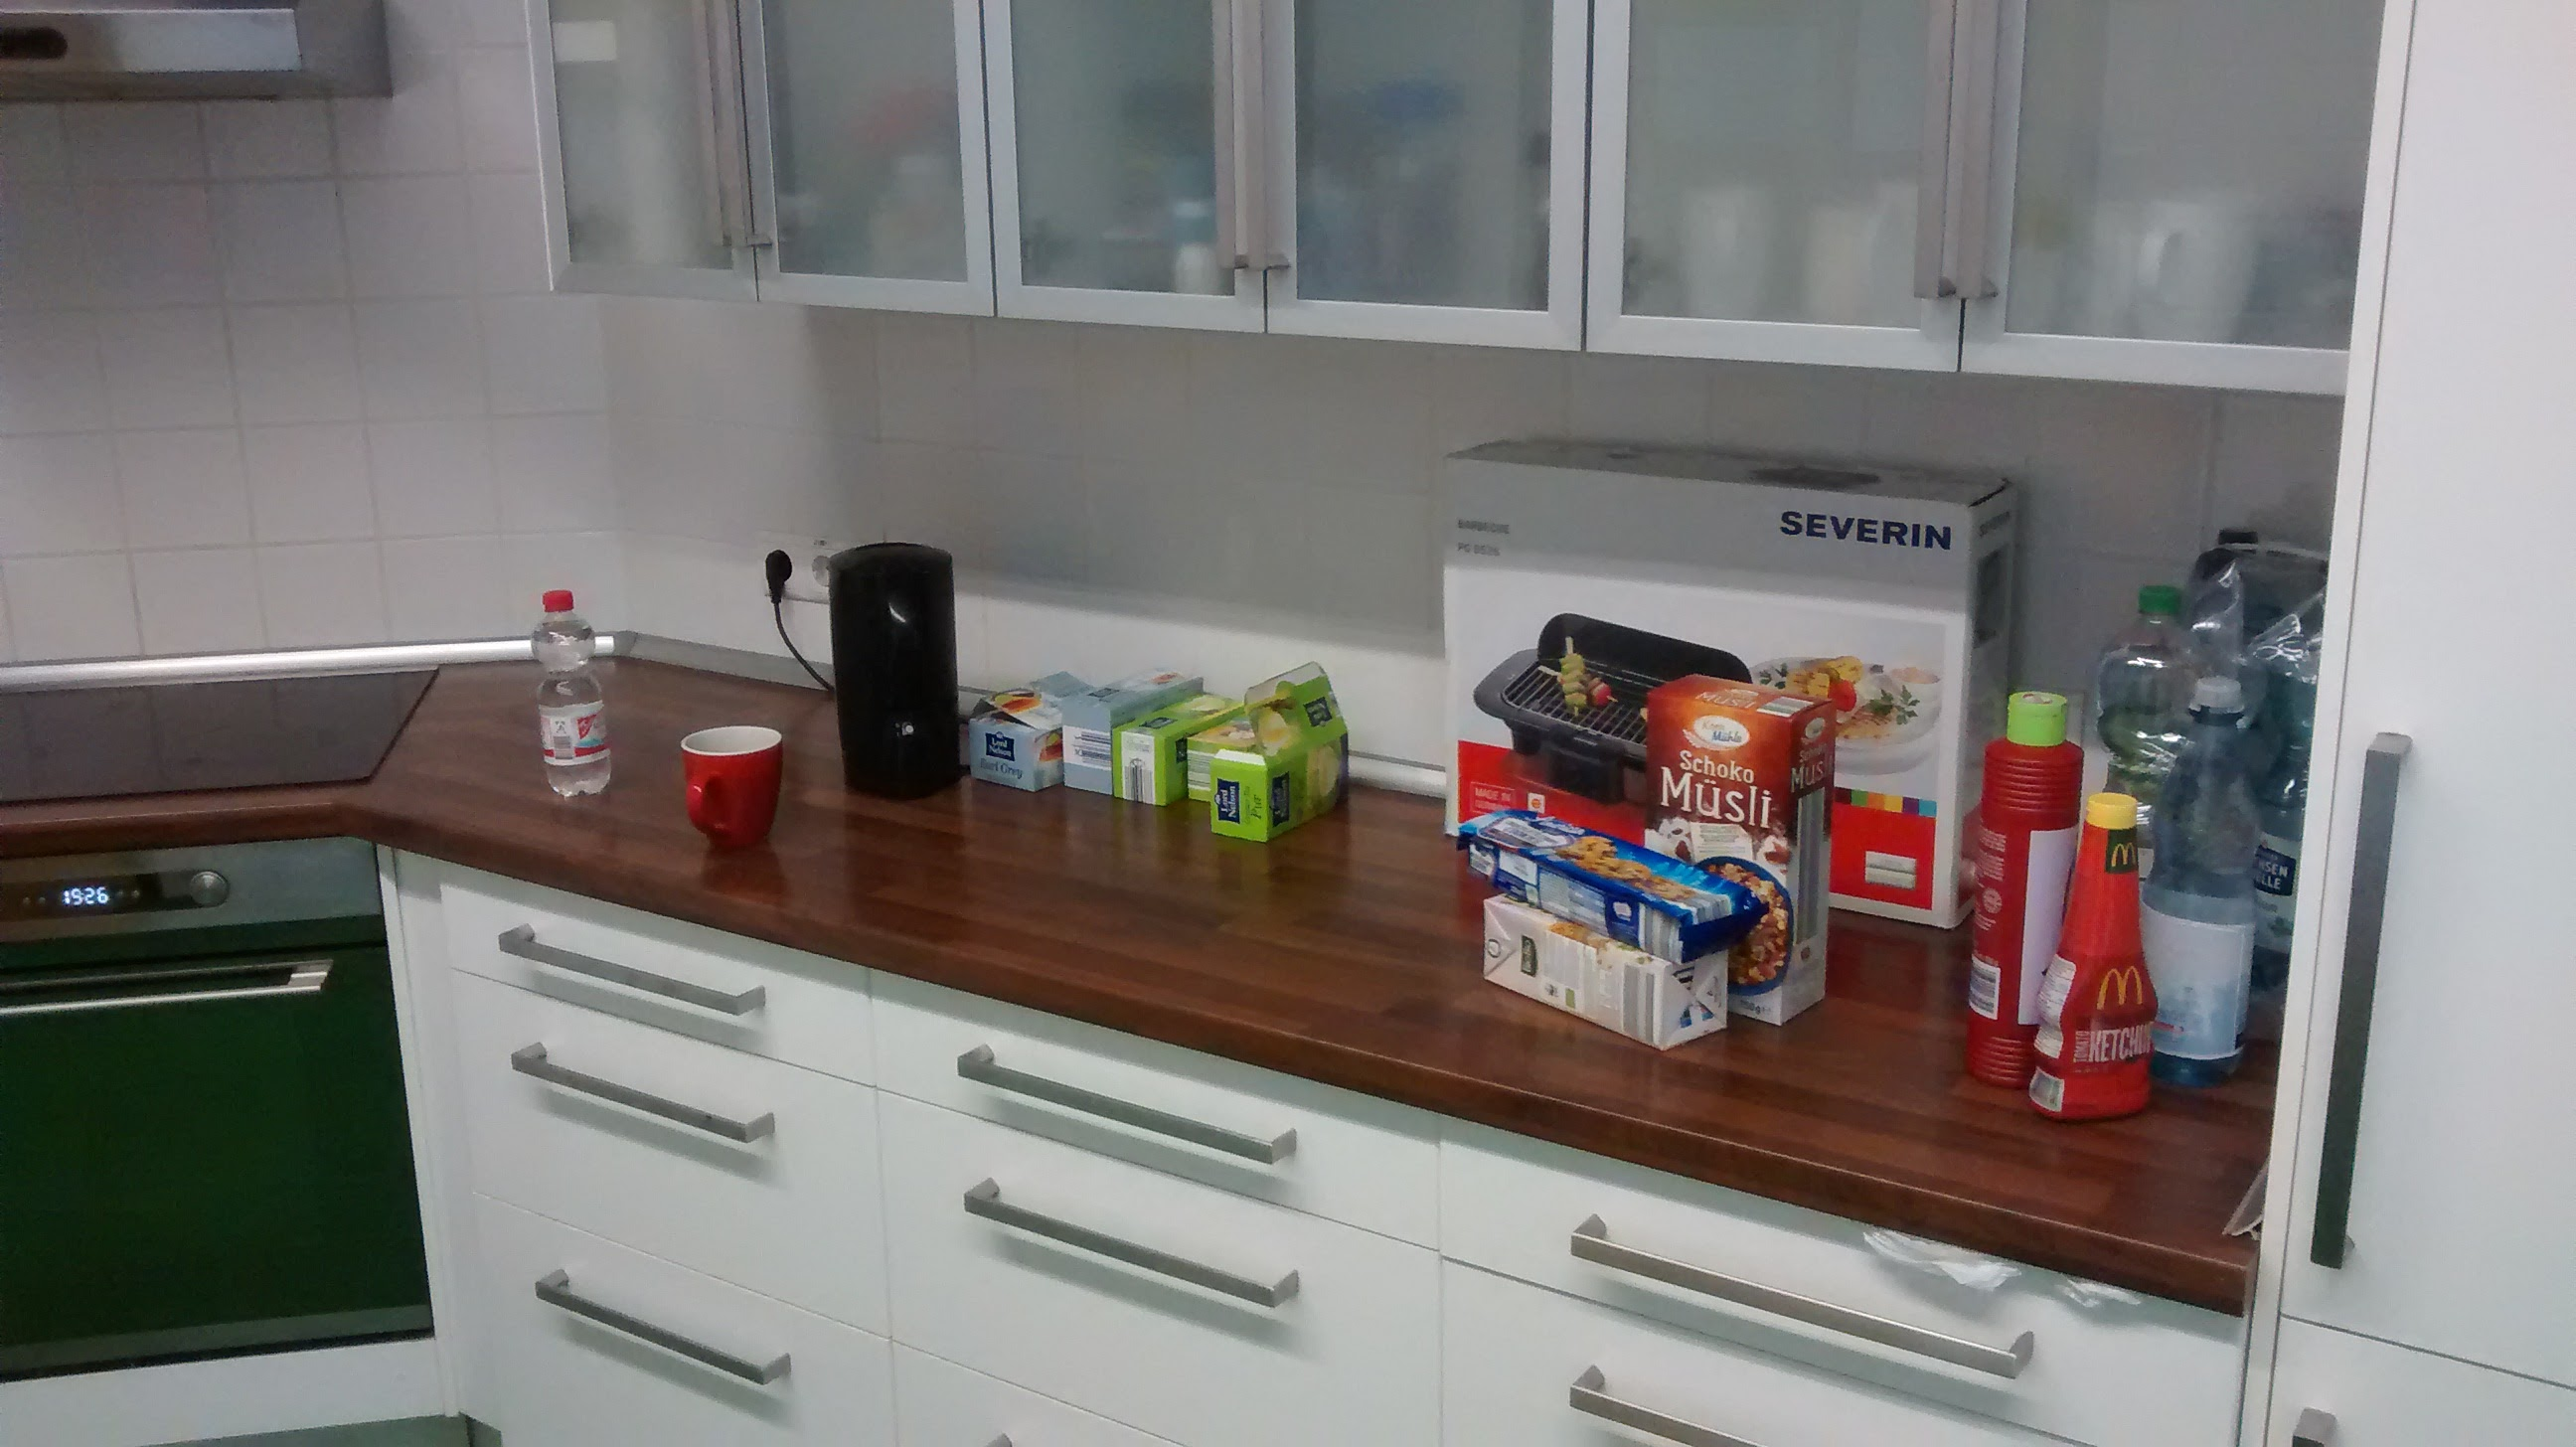
\includegraphics[width=\textwidth]{images/counter-top.jpg}
        \caption{counter-top}
        \label{fig:counter-top}
    \end{subfigure}
    \caption{Different possible object locations}\label{fig:alllocations}
\end{figure}
\begin{figure}
    \centering
    \begin{subfigure}[b]{0.3\textwidth}
        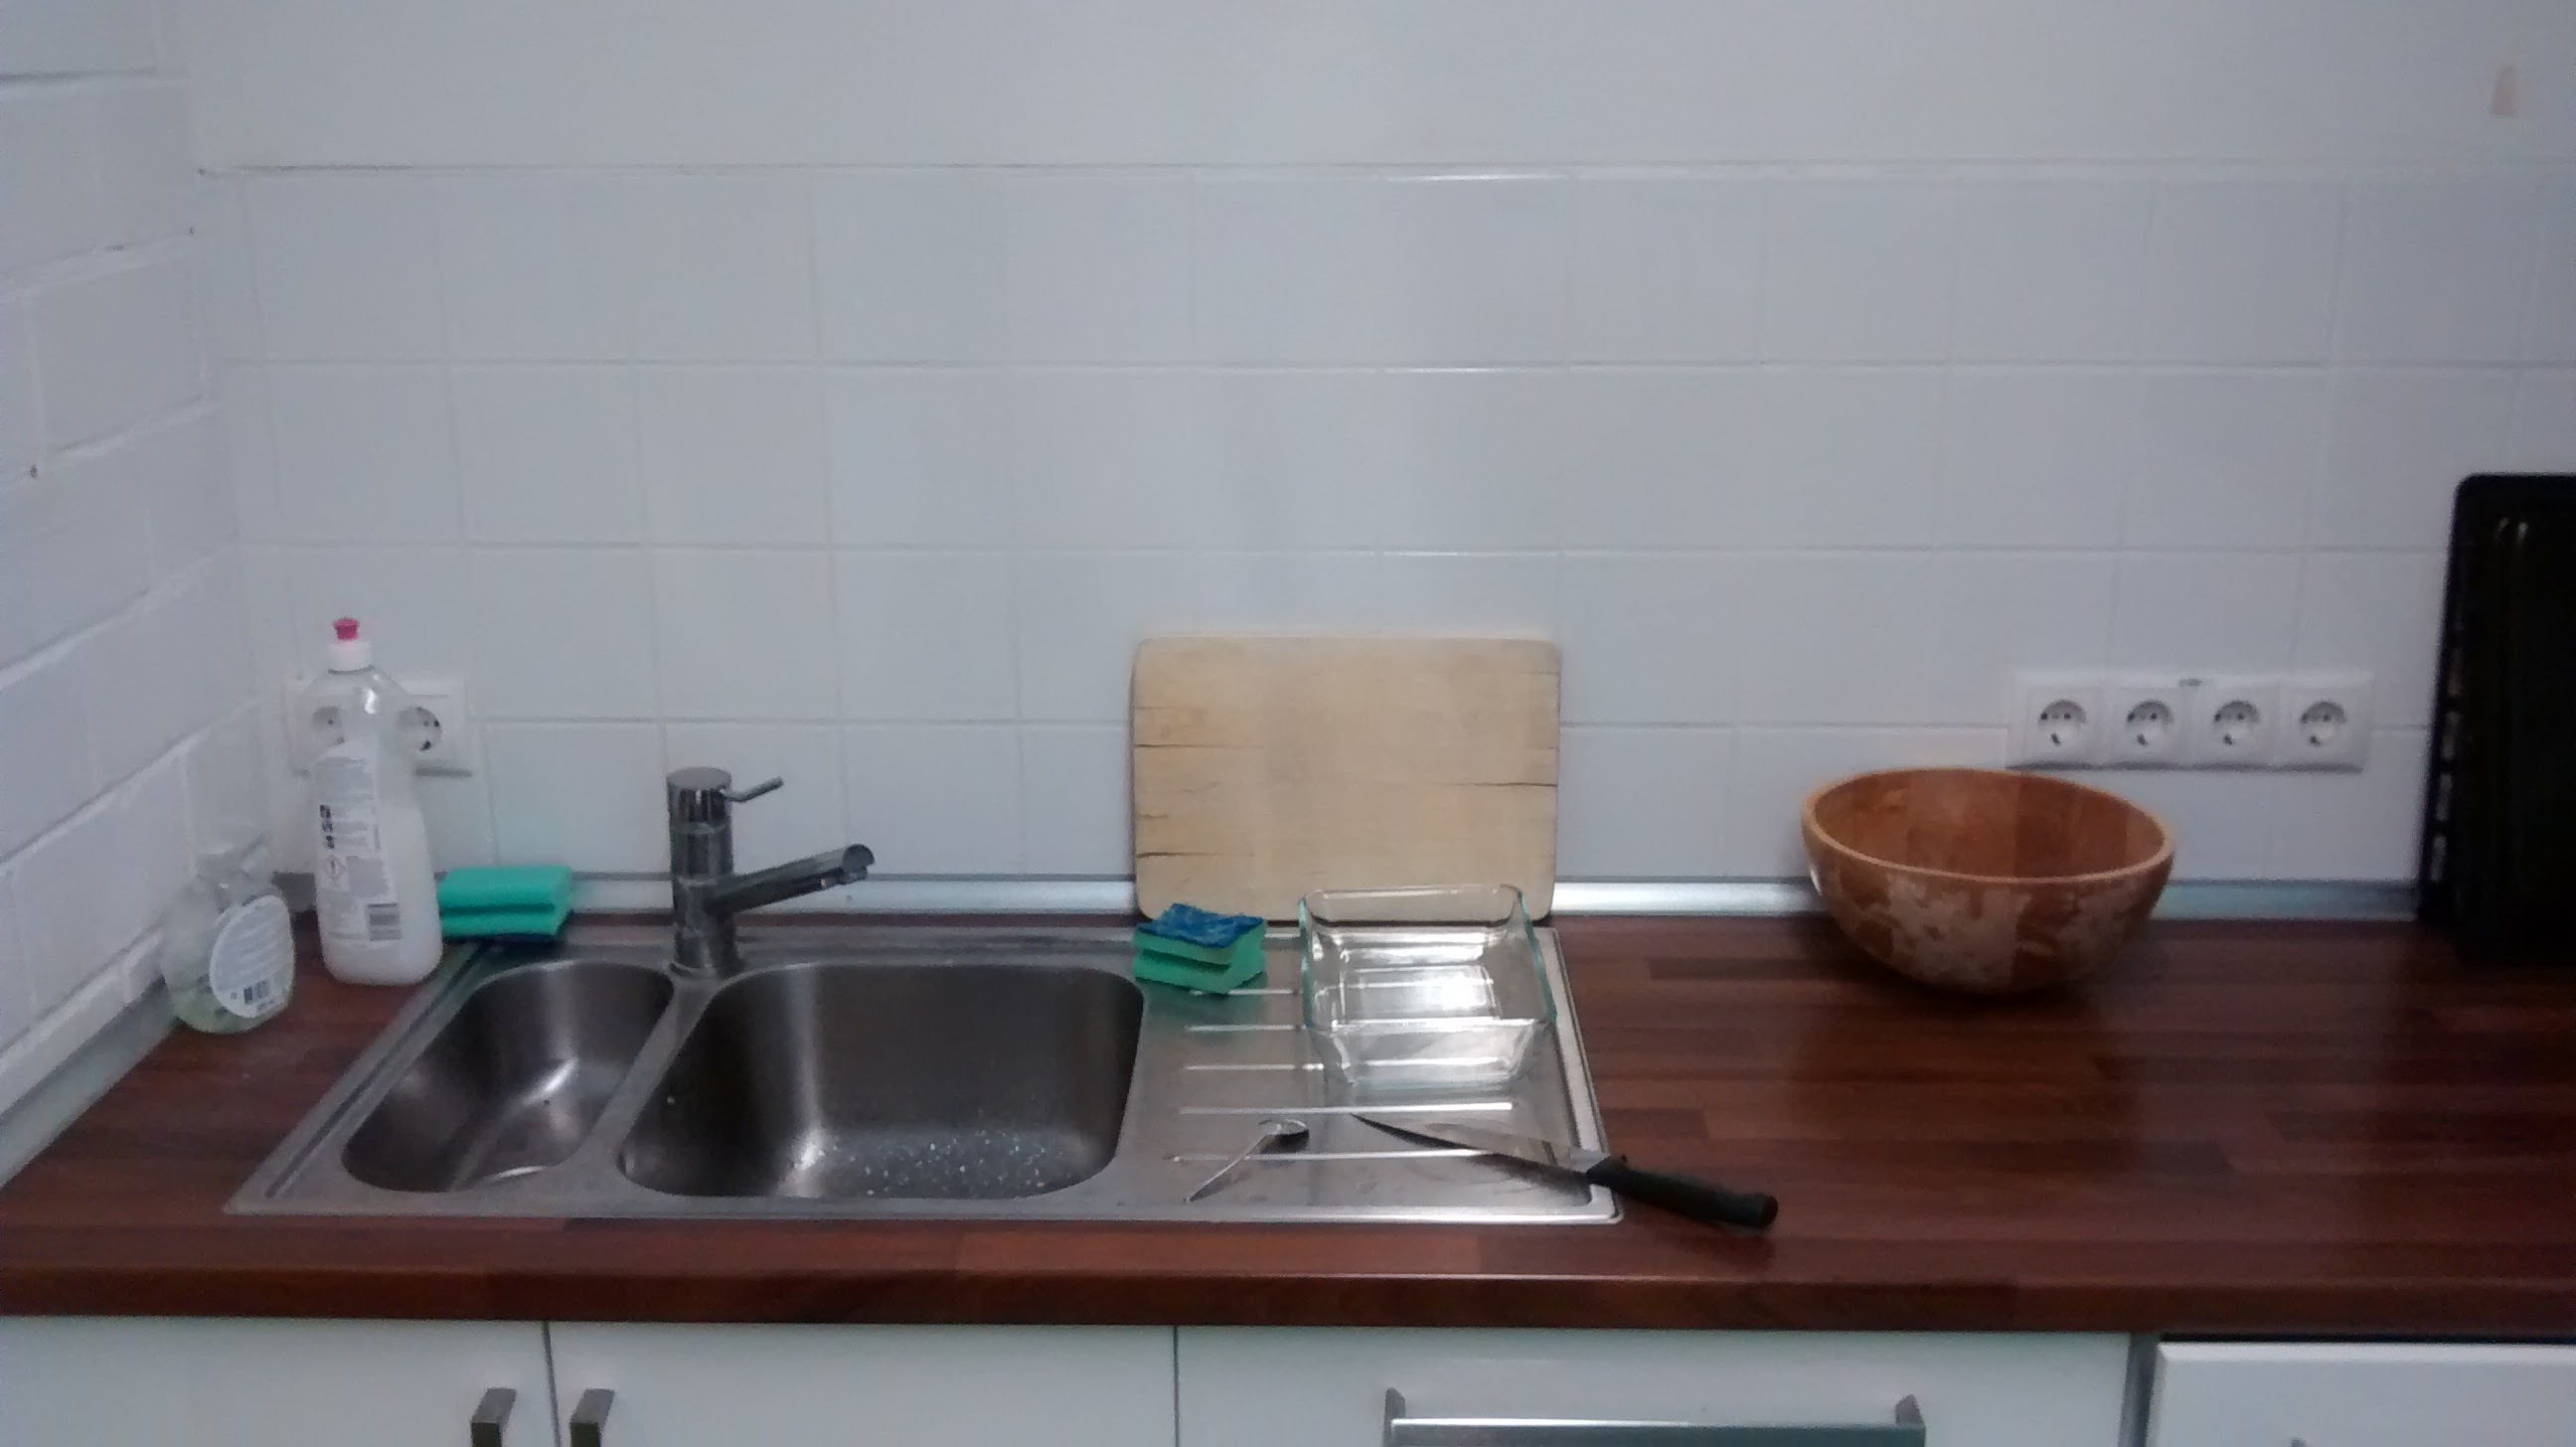
\includegraphics[width=\textwidth]{images/sink.jpg}
        \caption{Sink}
        \label{fig:sink}
    \end{subfigure}
    ~ %add desired spacing between images, e. g. ~, \quad, \qquad, \hfill etc. 
      %(or a blank line to force the subfigure onto a new line)
    \begin{subfigure}[b]{0.3\textwidth}
        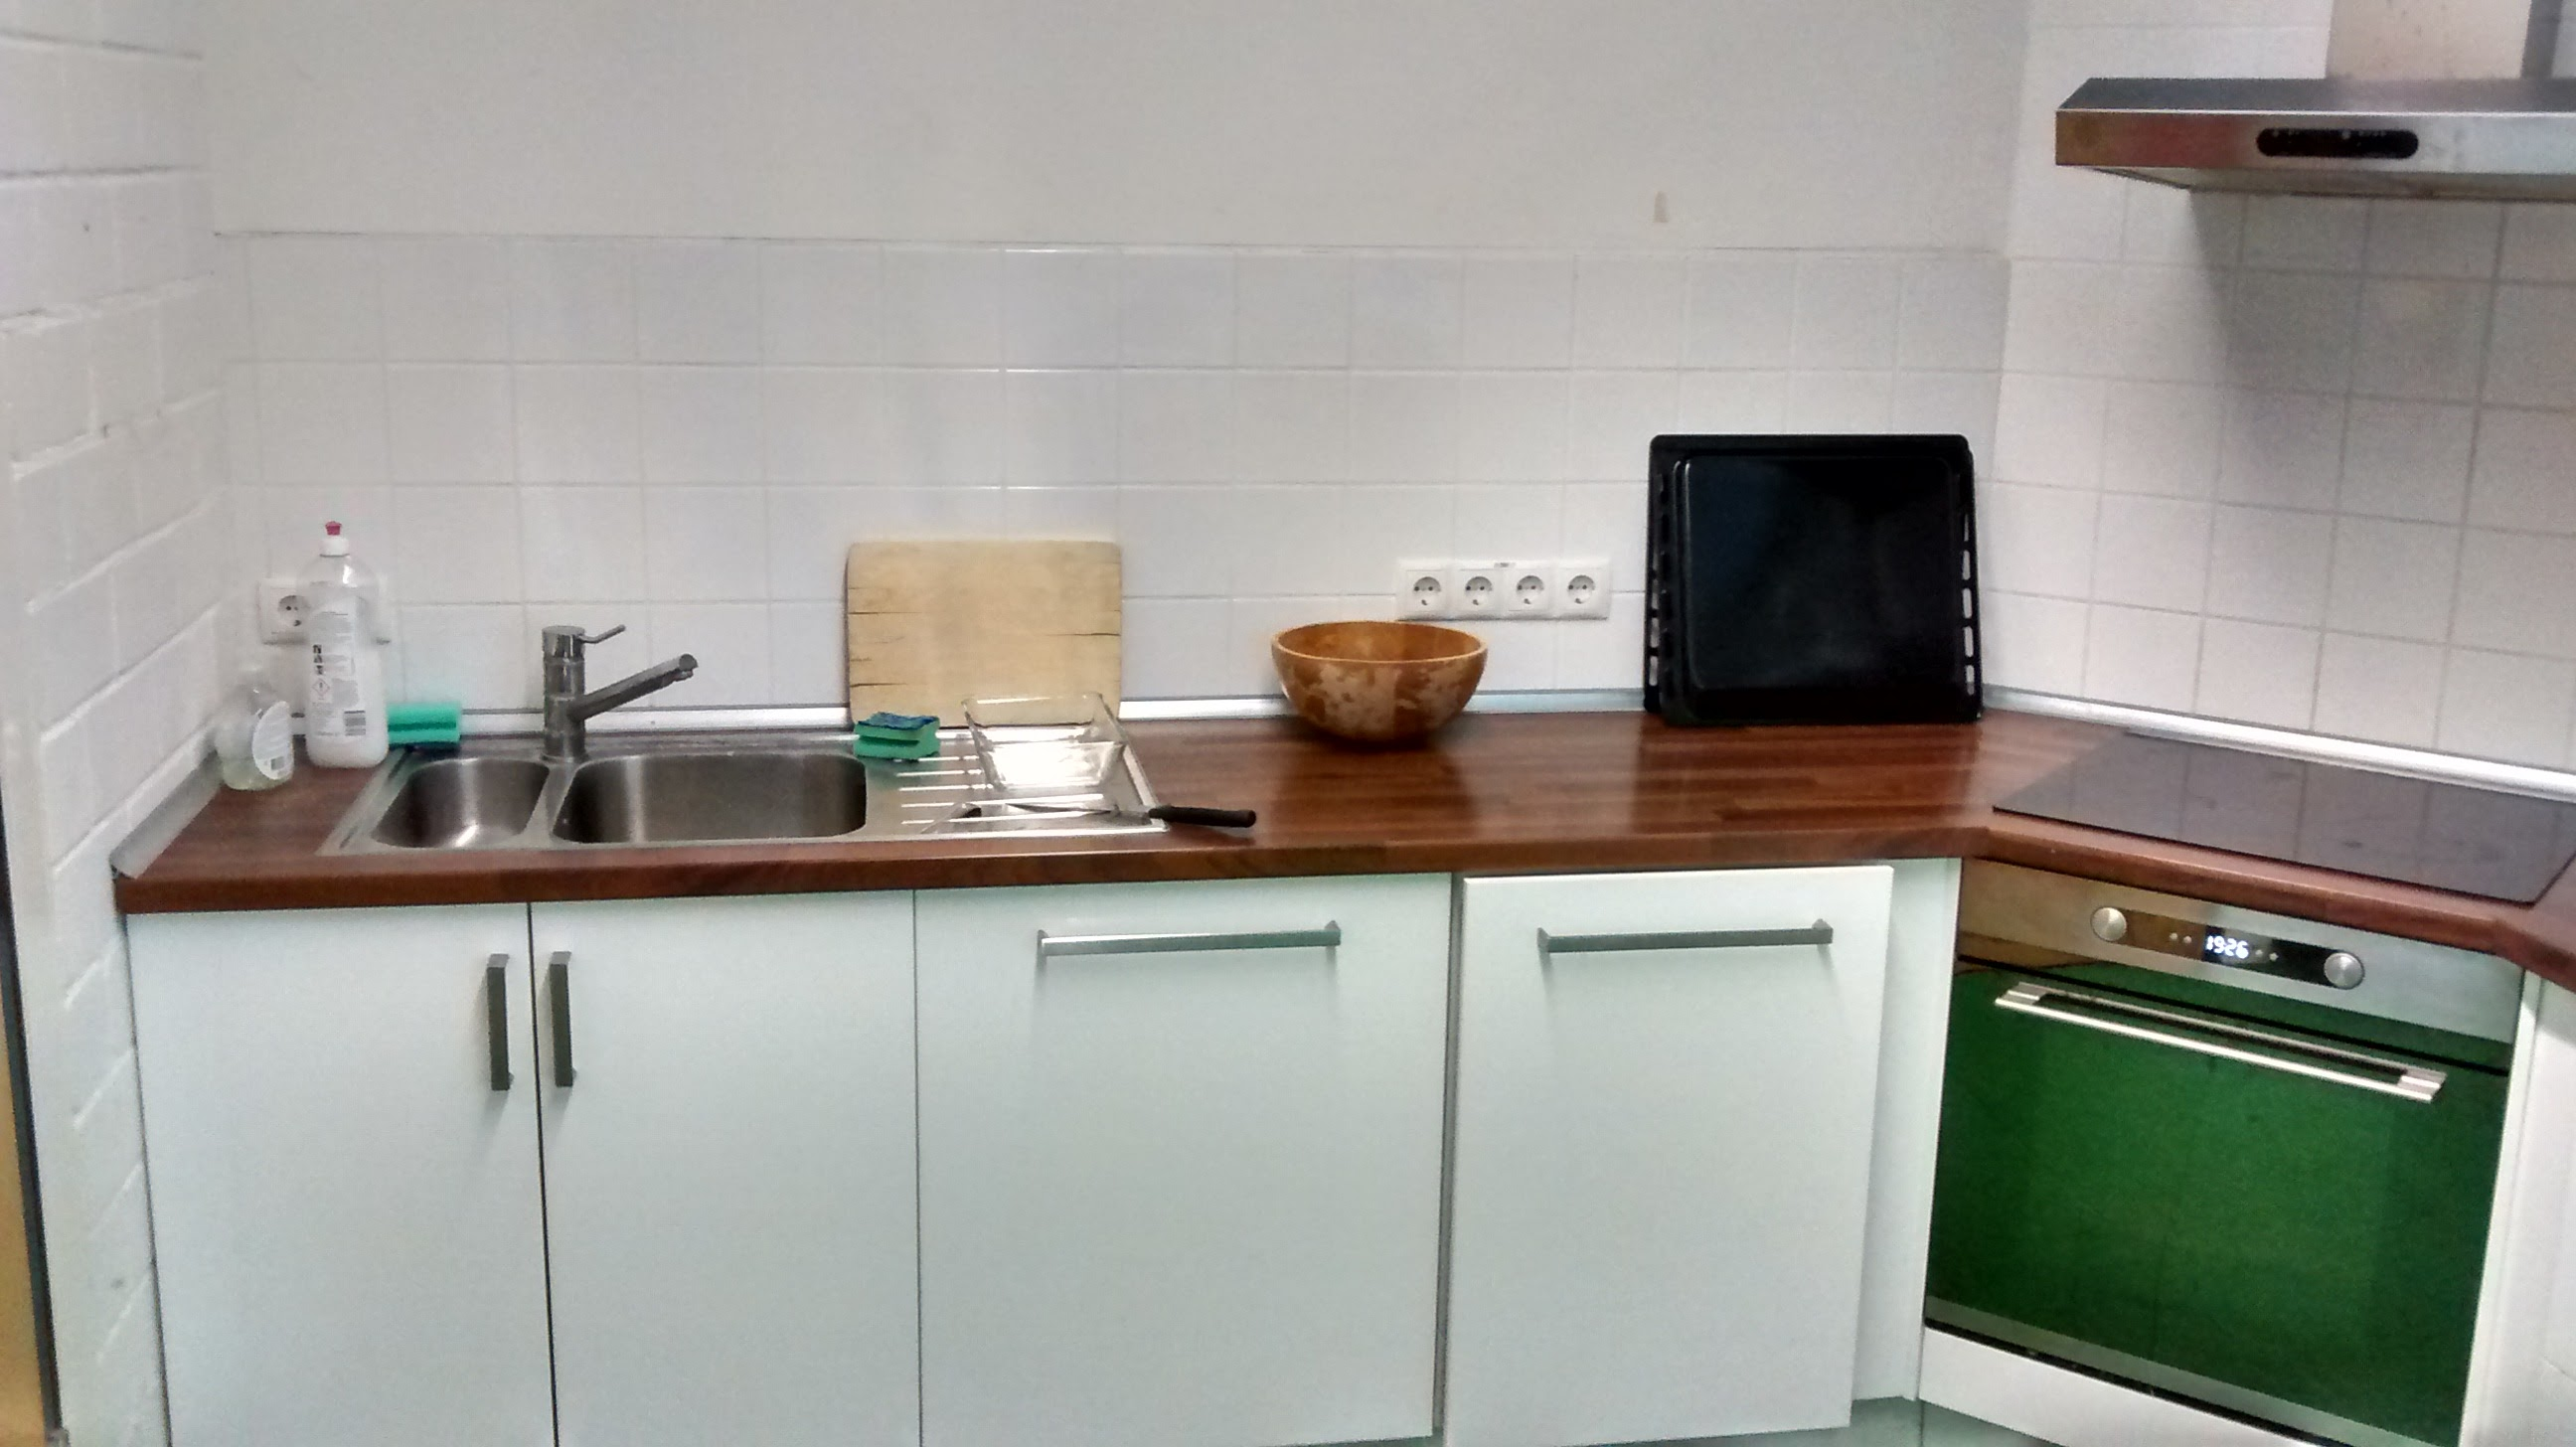
\includegraphics[width=\textwidth]{images/stove.jpg}
        \caption{Stove}
        \label{fig:stove}
    \end{subfigure}
    ~ %add desired spacing between images, e. g. ~, \quad, \qquad, \hfill etc. 
    %(or a blank line to force the subfigure onto a new line)
    \begin{subfigure}[b]{0.3\textwidth}
        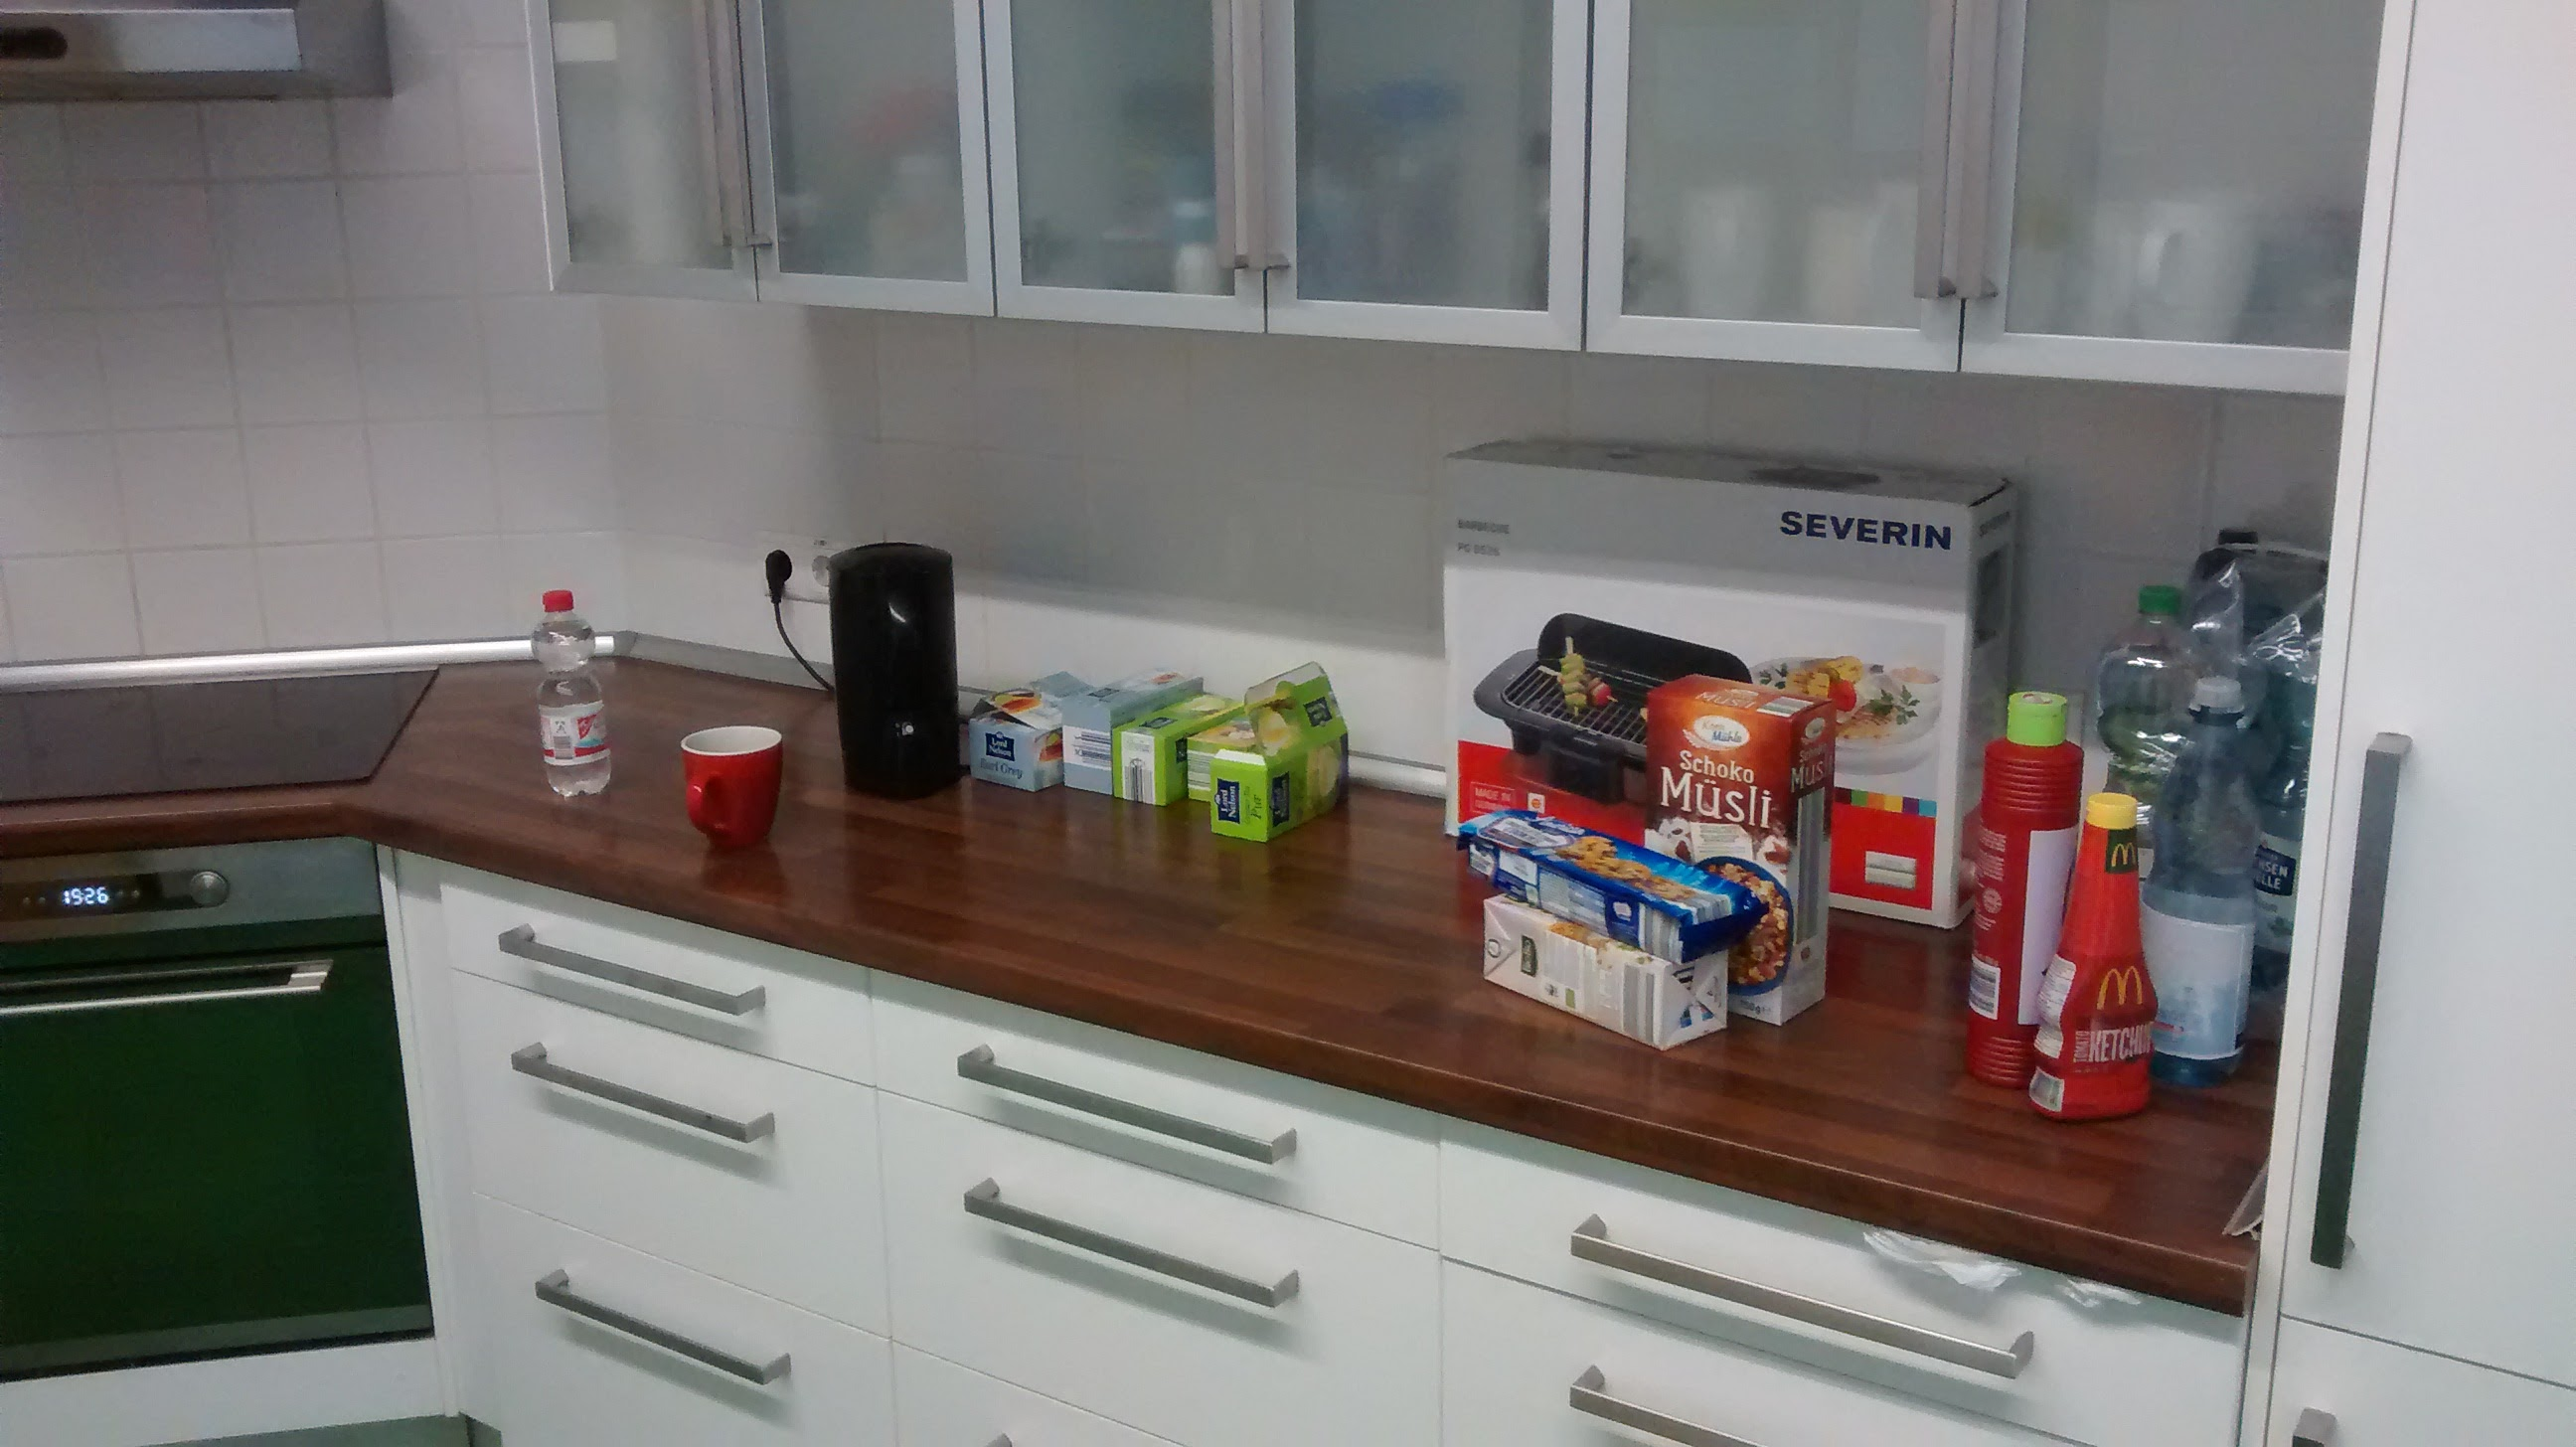
\includegraphics[width=\textwidth]{images/counter-top.jpg}
        \caption{counter-top}
        \label{fig:counter-top}
    \end{subfigure}
    \caption{Different possible object locations}\label{fig:alllocations}
\end{figure}
\begin{figure}
    \centering
    \begin{subfigure}[b]{0.3\textwidth}
        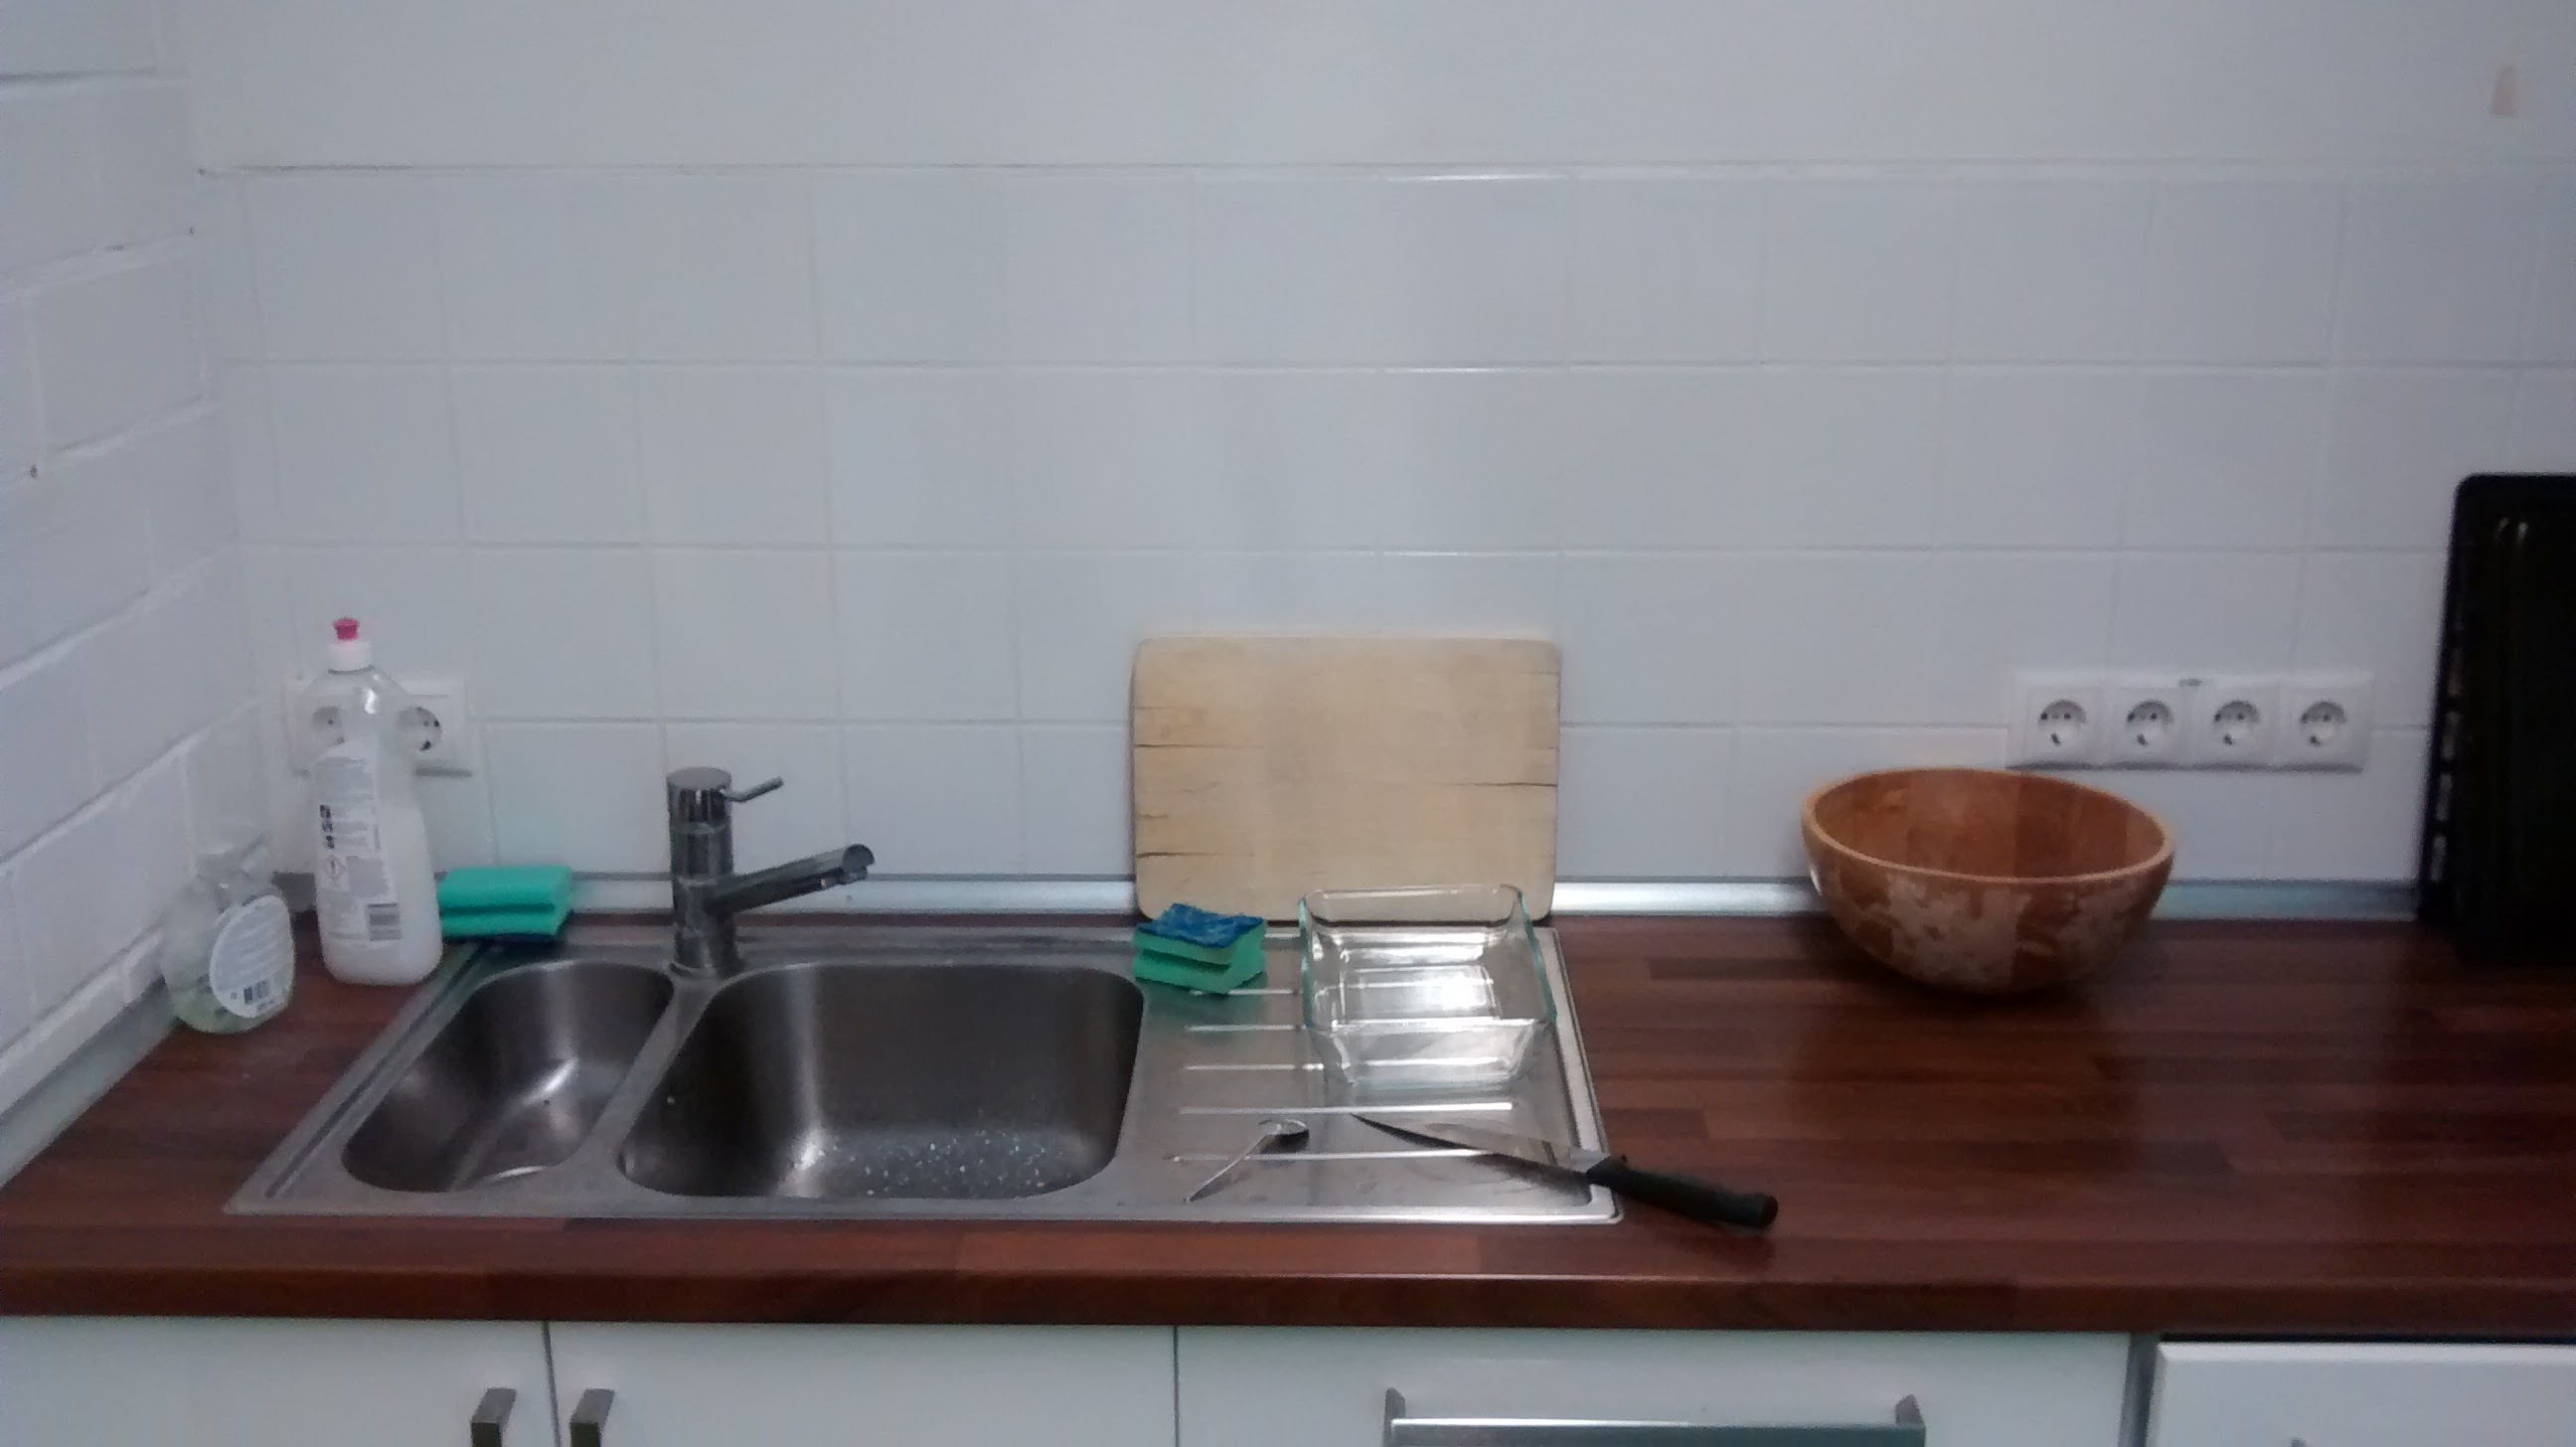
\includegraphics[width=\textwidth]{images/sink.jpg}
        \caption{Sink}
        \label{fig:sink}
    \end{subfigure}
    ~ %add desired spacing between images, e. g. ~, \quad, \qquad, \hfill etc. 
      %(or a blank line to force the subfigure onto a new line)
    \begin{subfigure}[b]{0.3\textwidth}
        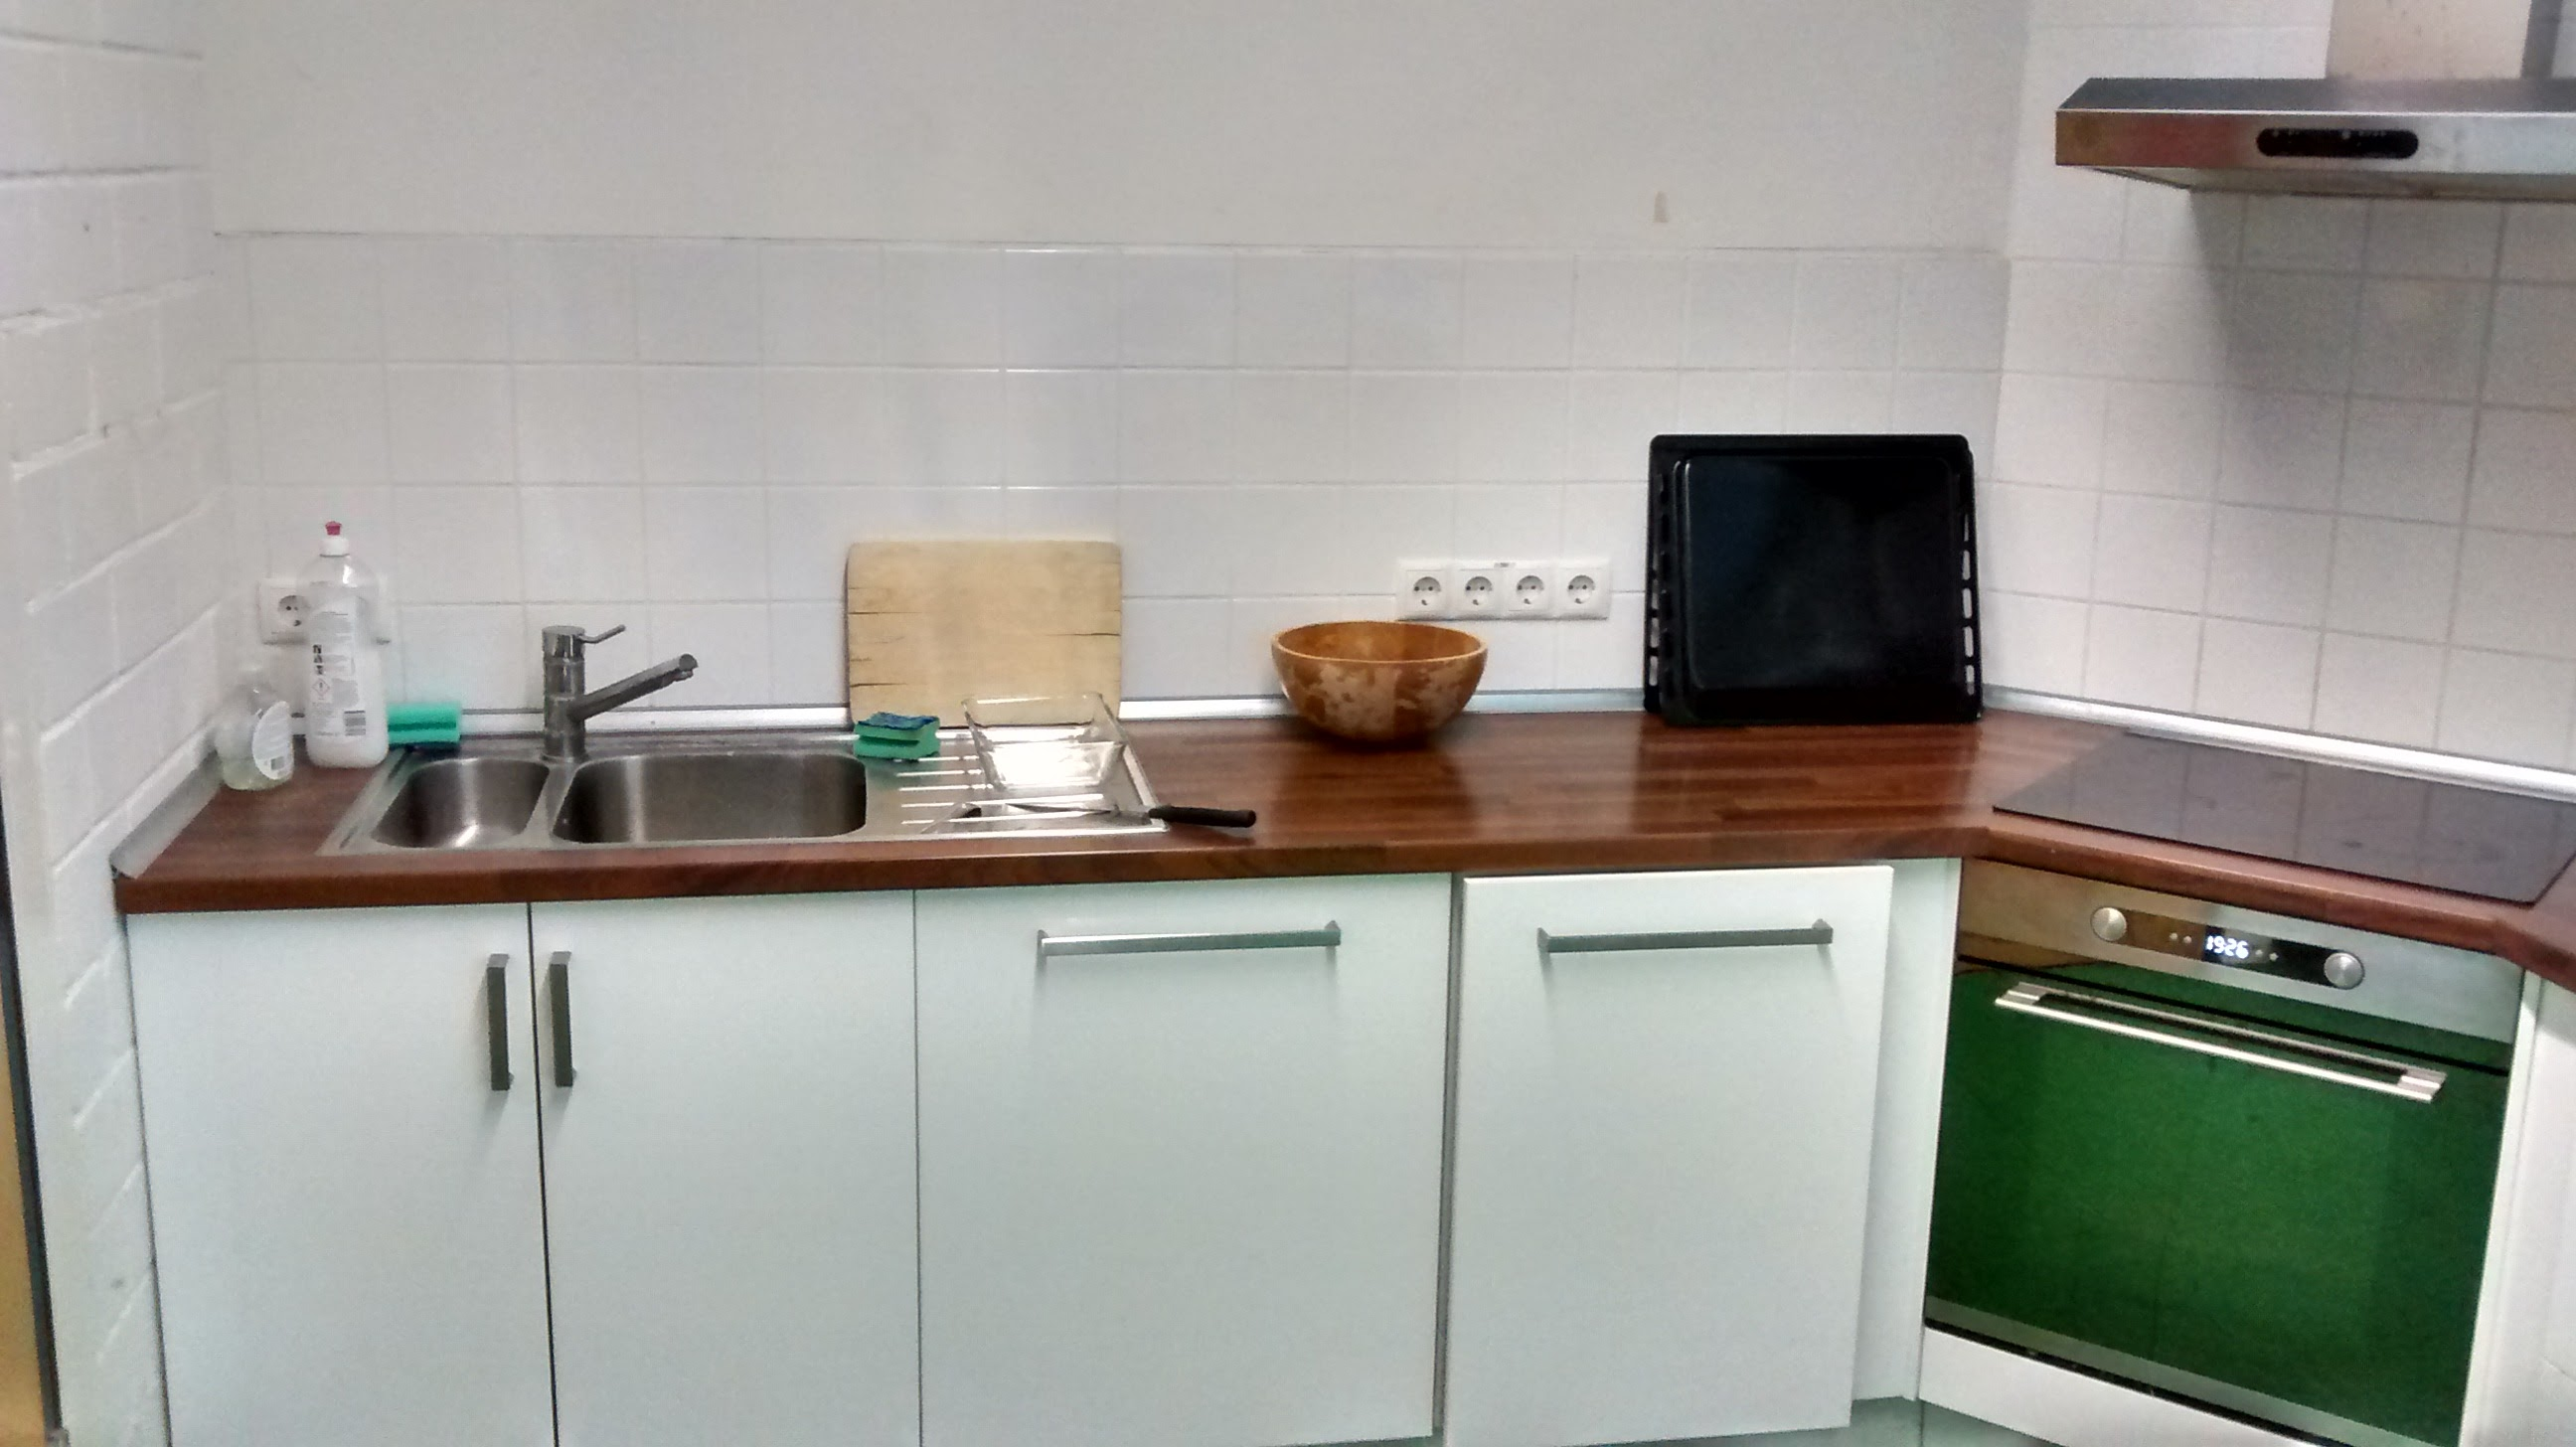
\includegraphics[width=\textwidth]{images/stove.jpg}
        \caption{Stove}
        \label{fig:stove}
    \end{subfigure}
    ~ %add desired spacing between images, e. g. ~, \quad, \qquad, \hfill etc. 
    %(or a blank line to force the subfigure onto a new line)
    \begin{subfigure}[b]{0.3\textwidth}
        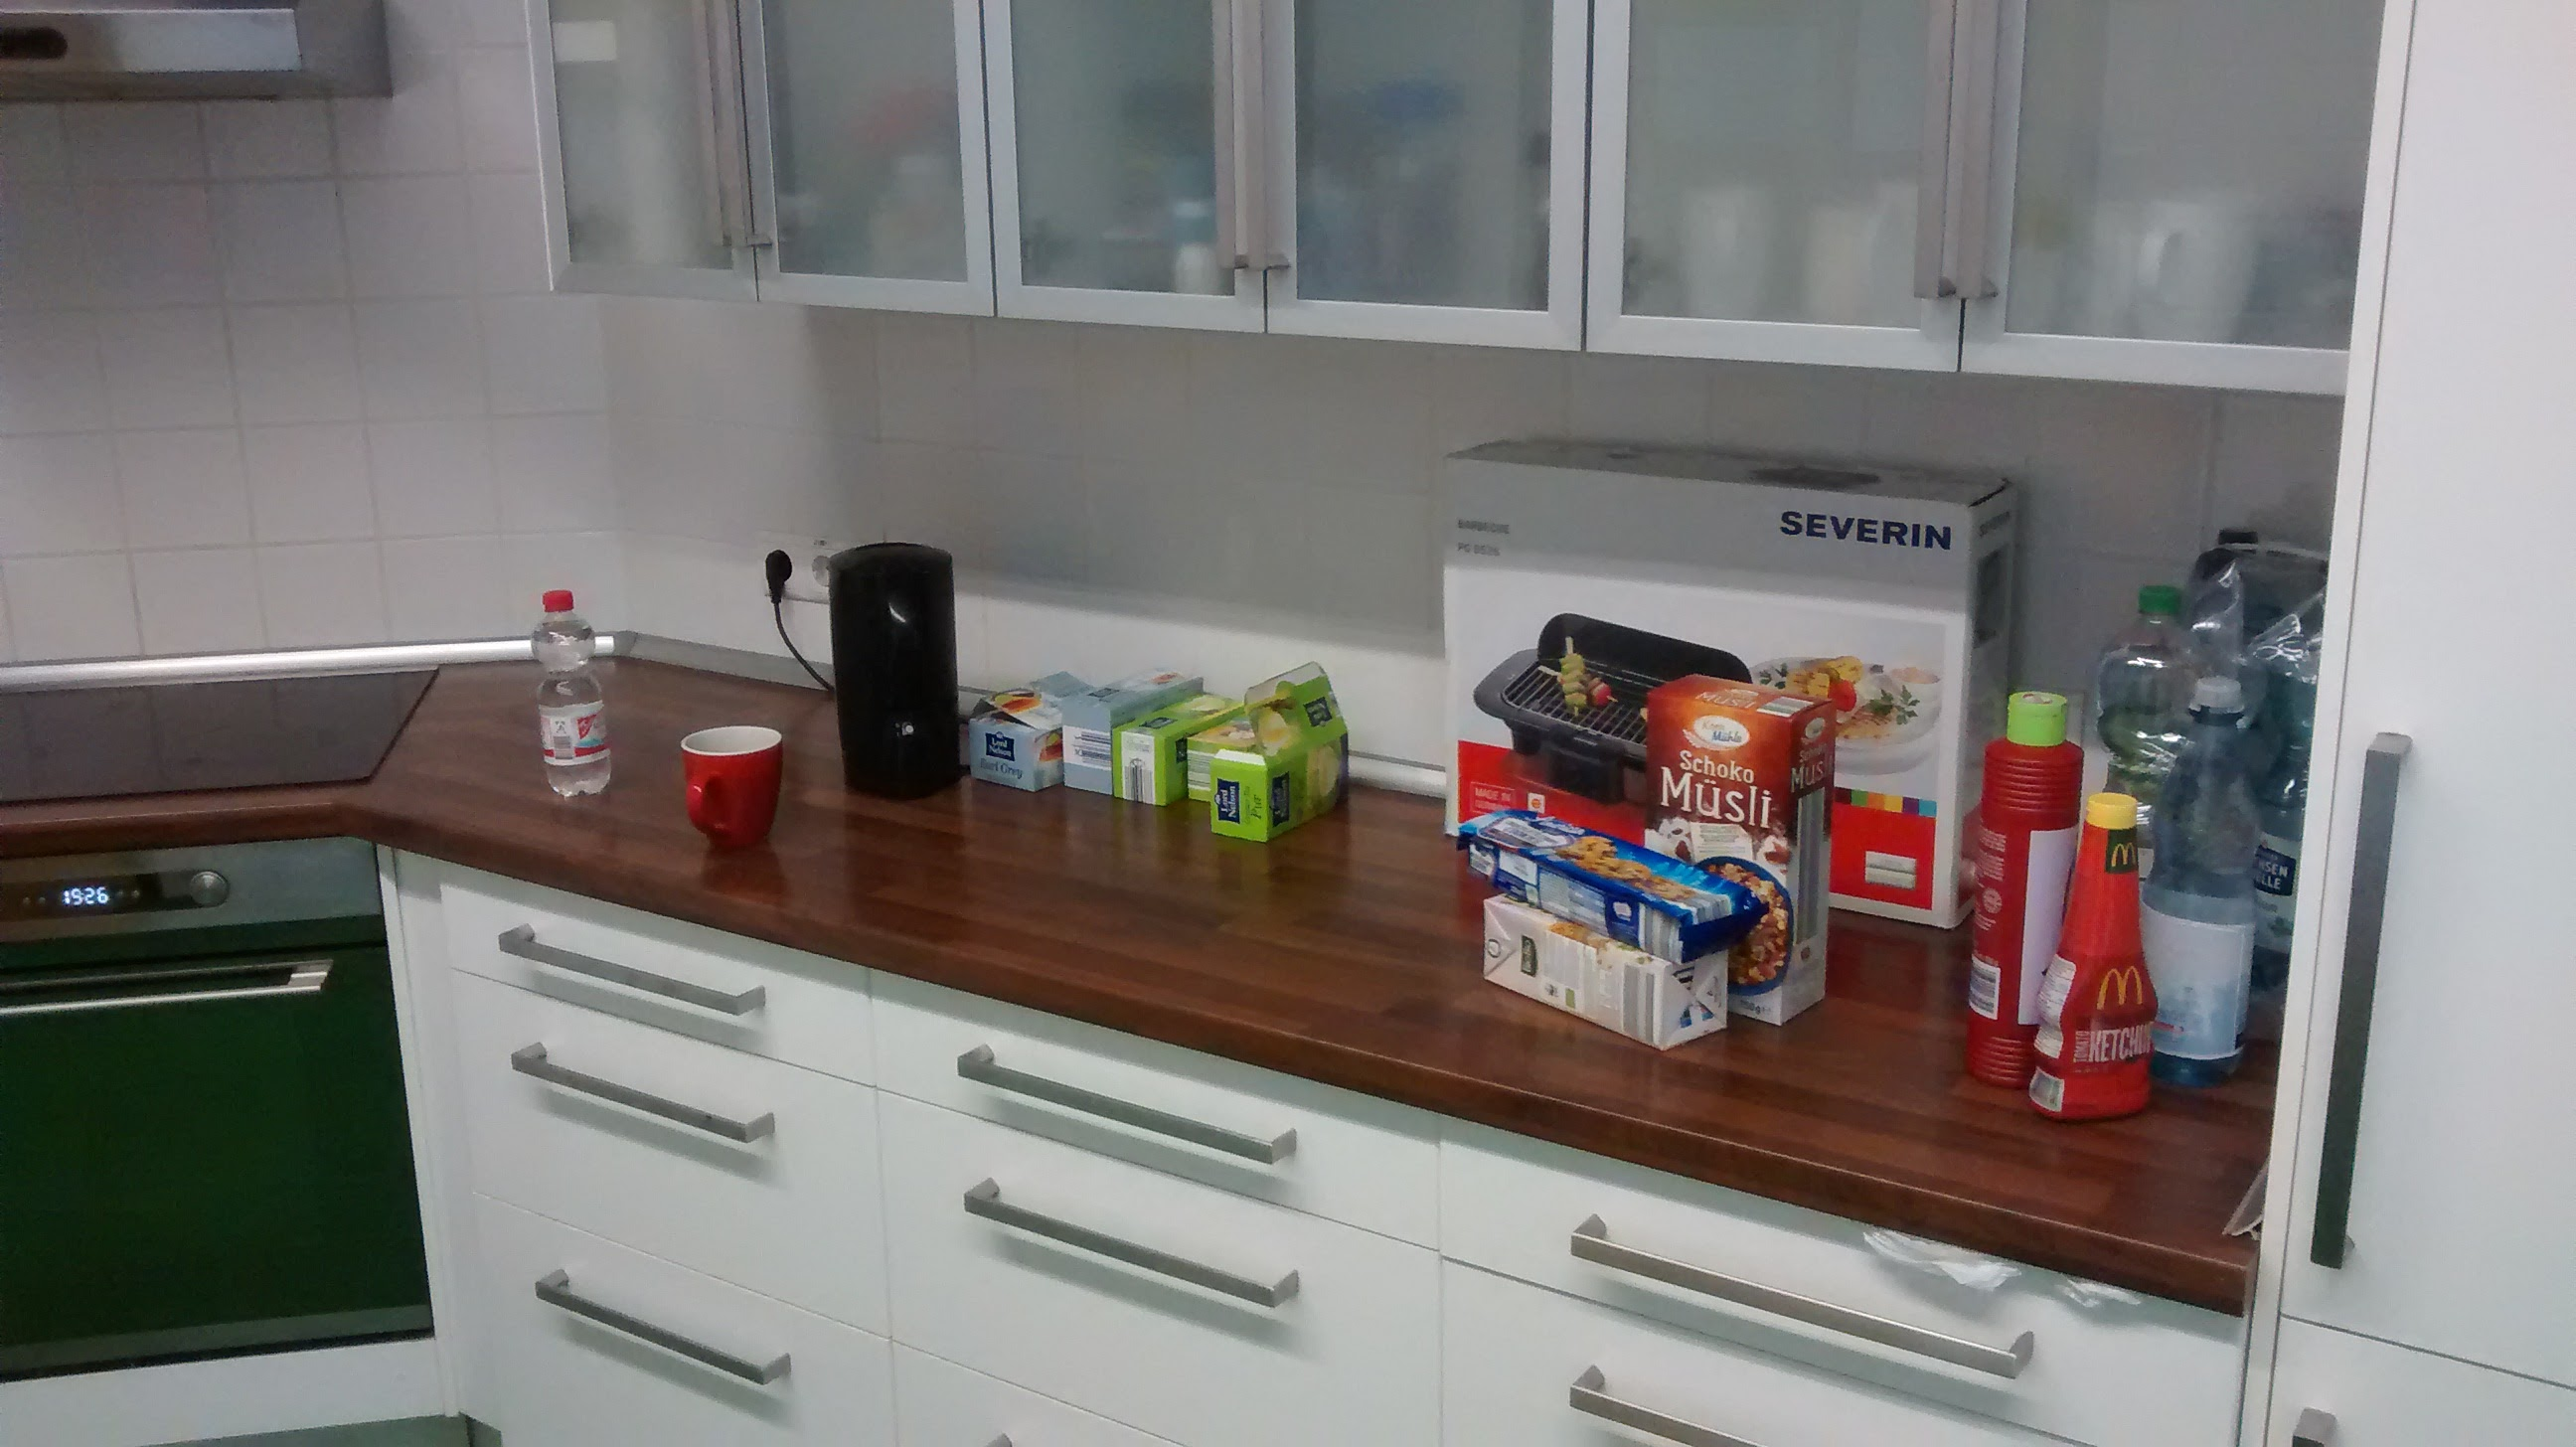
\includegraphics[width=\textwidth]{images/counter-top.jpg}
        \caption{counter-top}
        \label{fig:counter-top}
    \end{subfigure}
    \caption{Different possible object locations}\label{fig:alllocations}
\end{figure}
\begin{figure}
    \centering
    \begin{subfigure}[b]{0.3\textwidth}
        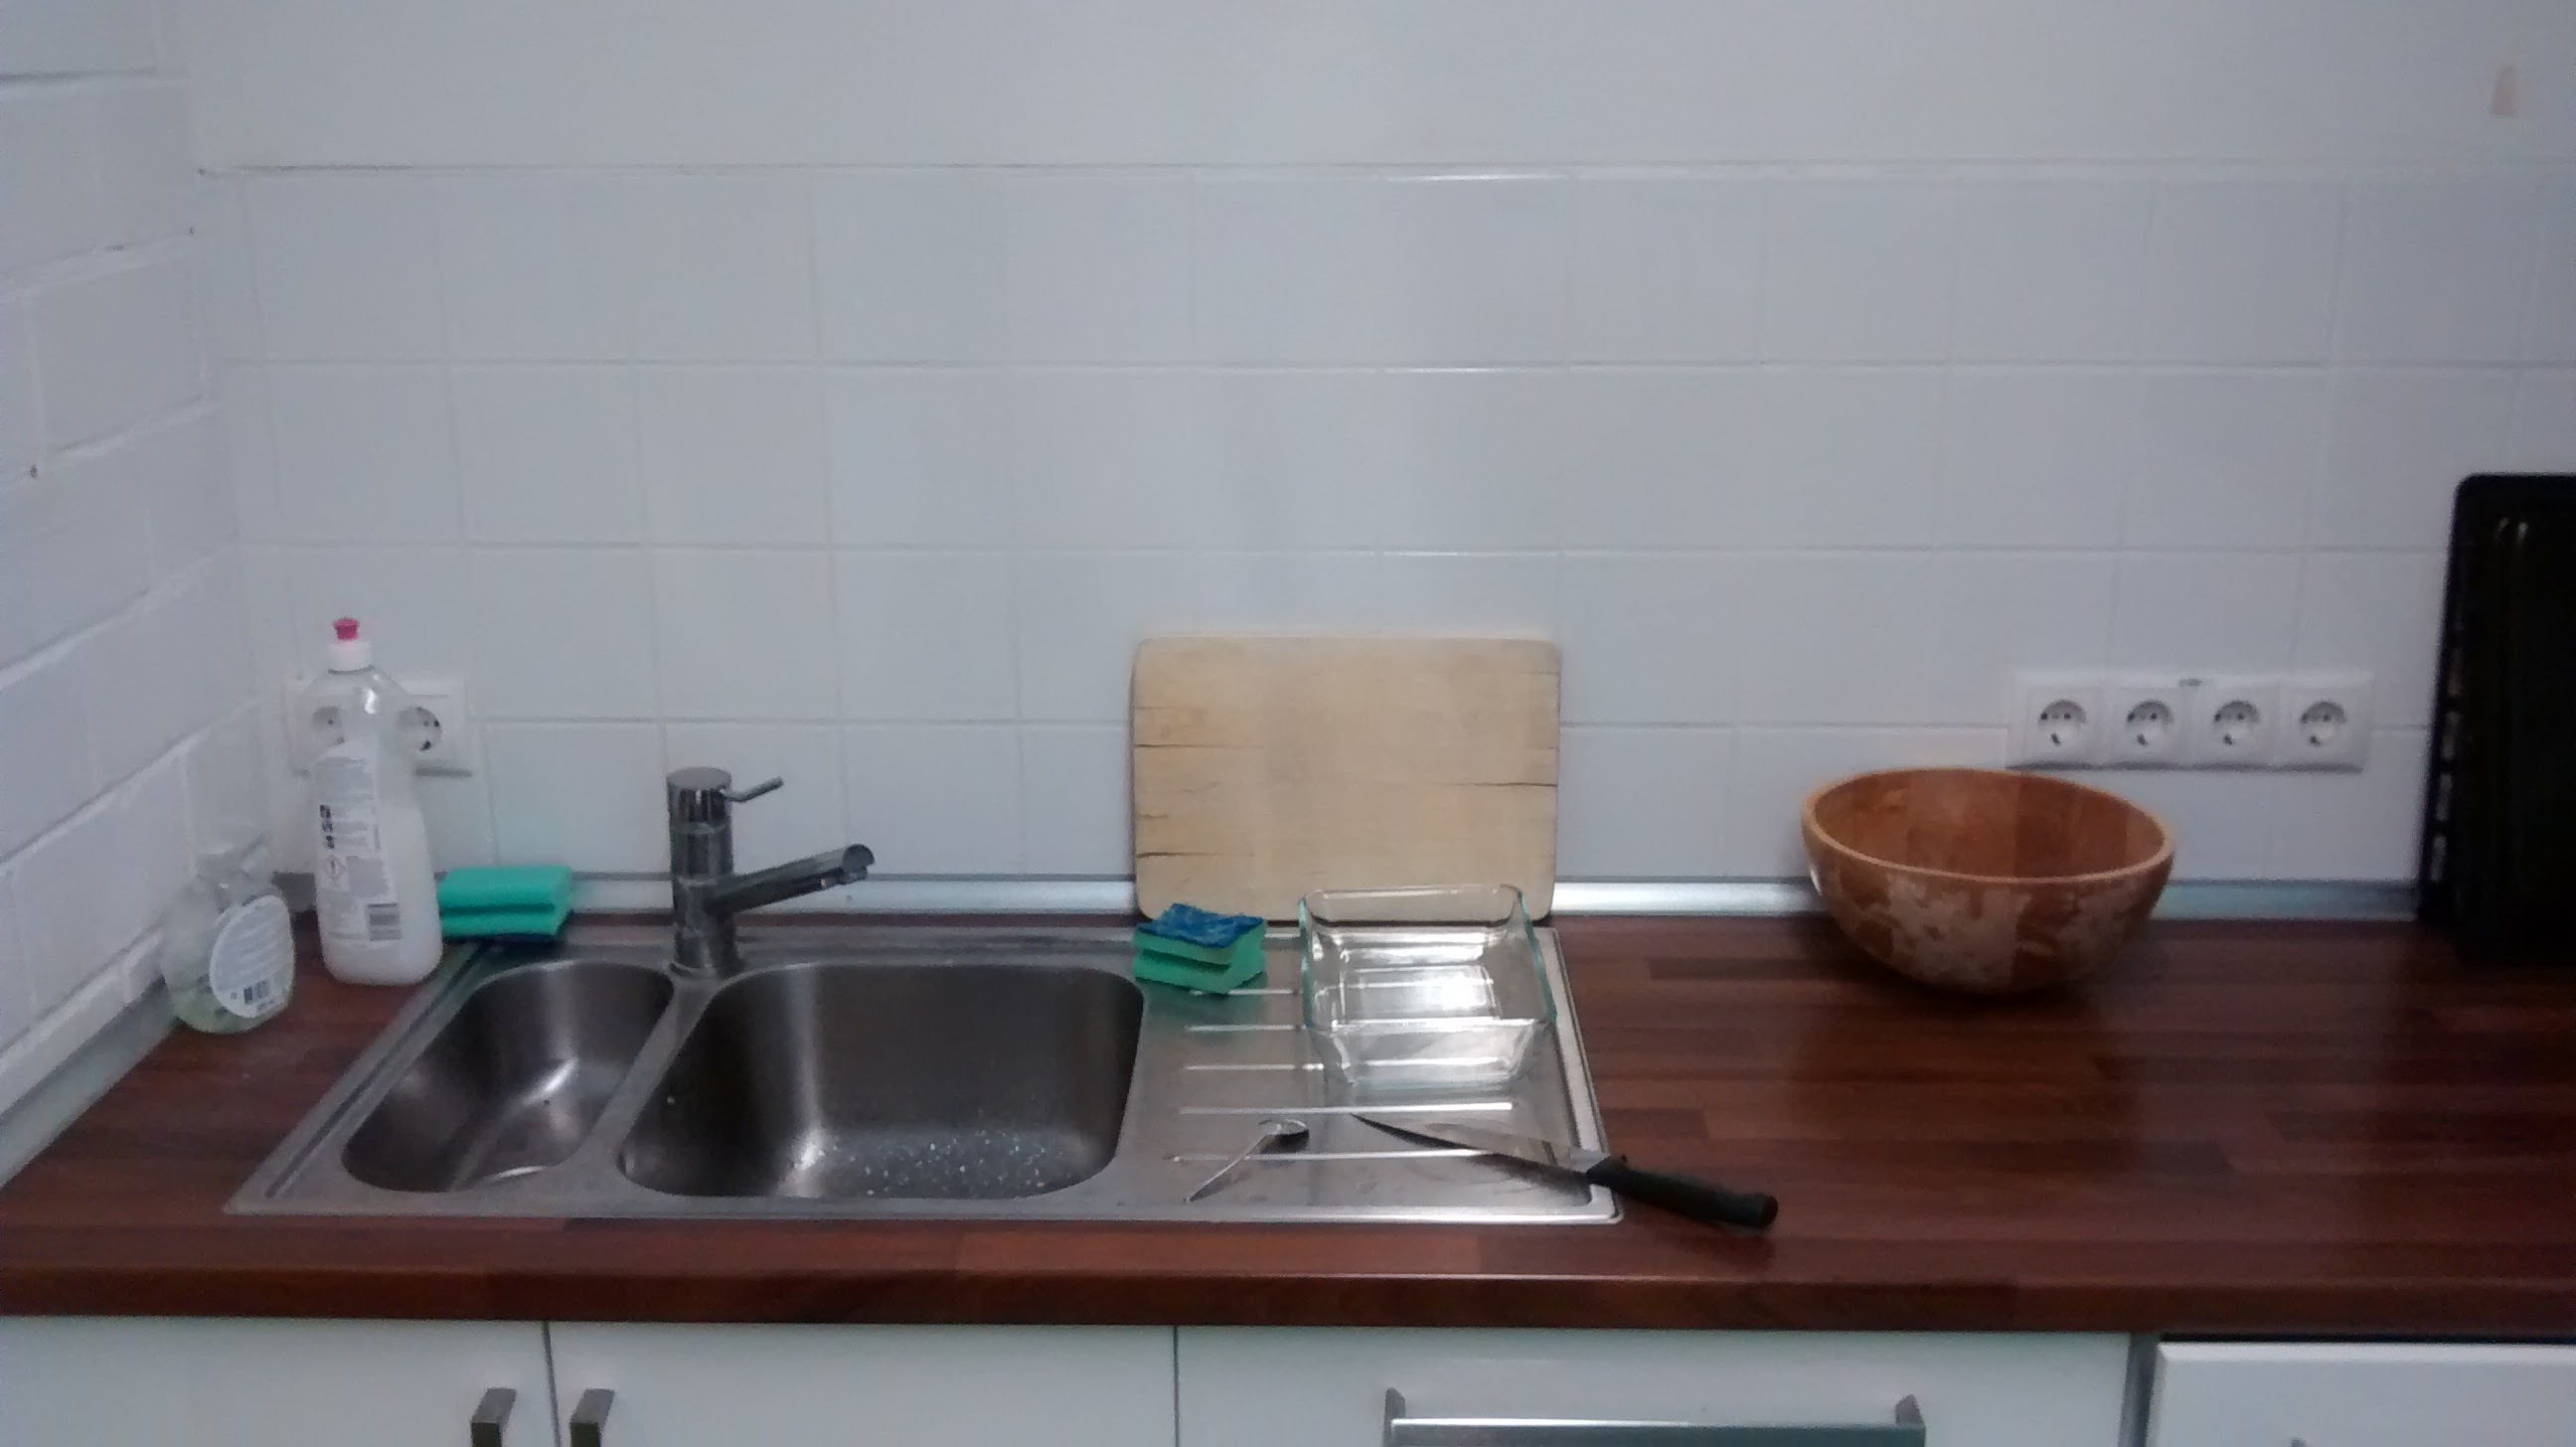
\includegraphics[width=\textwidth]{images/sink.jpg}
        \caption{Sink}
        \label{fig:sink}
    \end{subfigure}
    ~ %add desired spacing between images, e. g. ~, \quad, \qquad, \hfill etc. 
      %(or a blank line to force the subfigure onto a new line)
    \begin{subfigure}[b]{0.3\textwidth}
        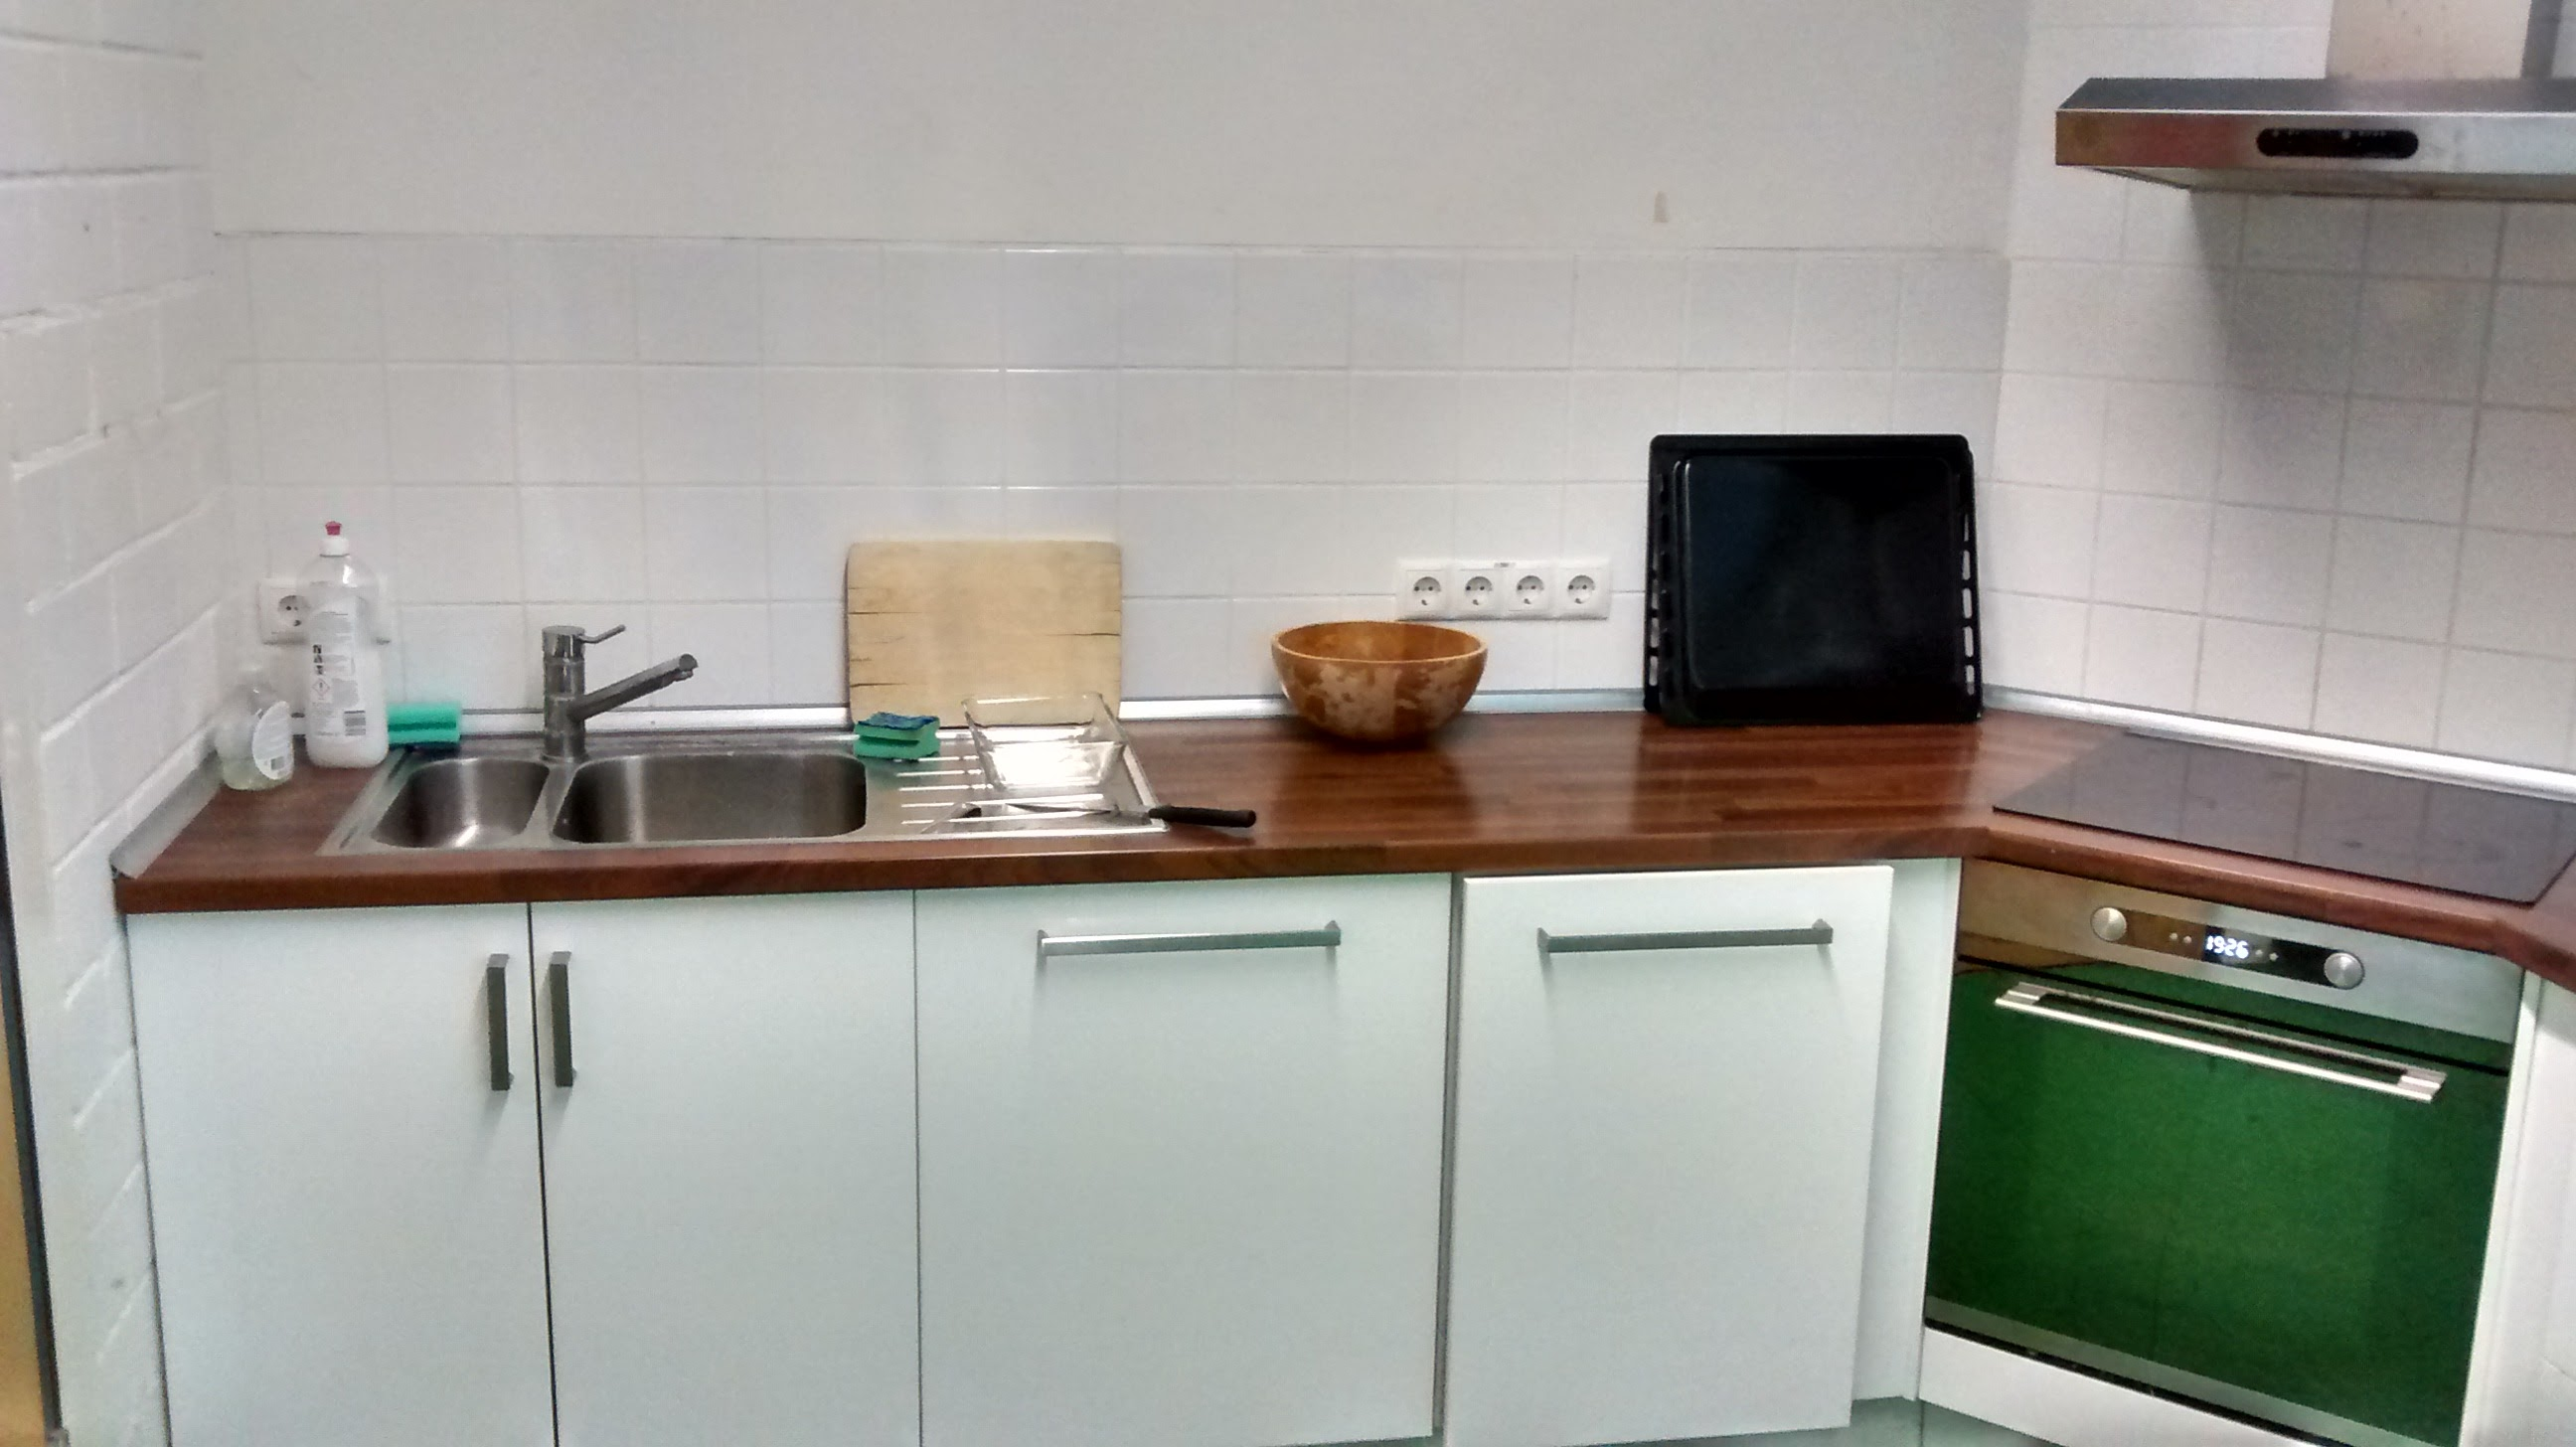
\includegraphics[width=\textwidth]{images/stove.jpg}
        \caption{Stove}
        \label{fig:stove}
    \end{subfigure}
    ~ %add desired spacing between images, e. g. ~, \quad, \qquad, \hfill etc. 
    %(or a blank line to force the subfigure onto a new line)
    \begin{subfigure}[b]{0.3\textwidth}
        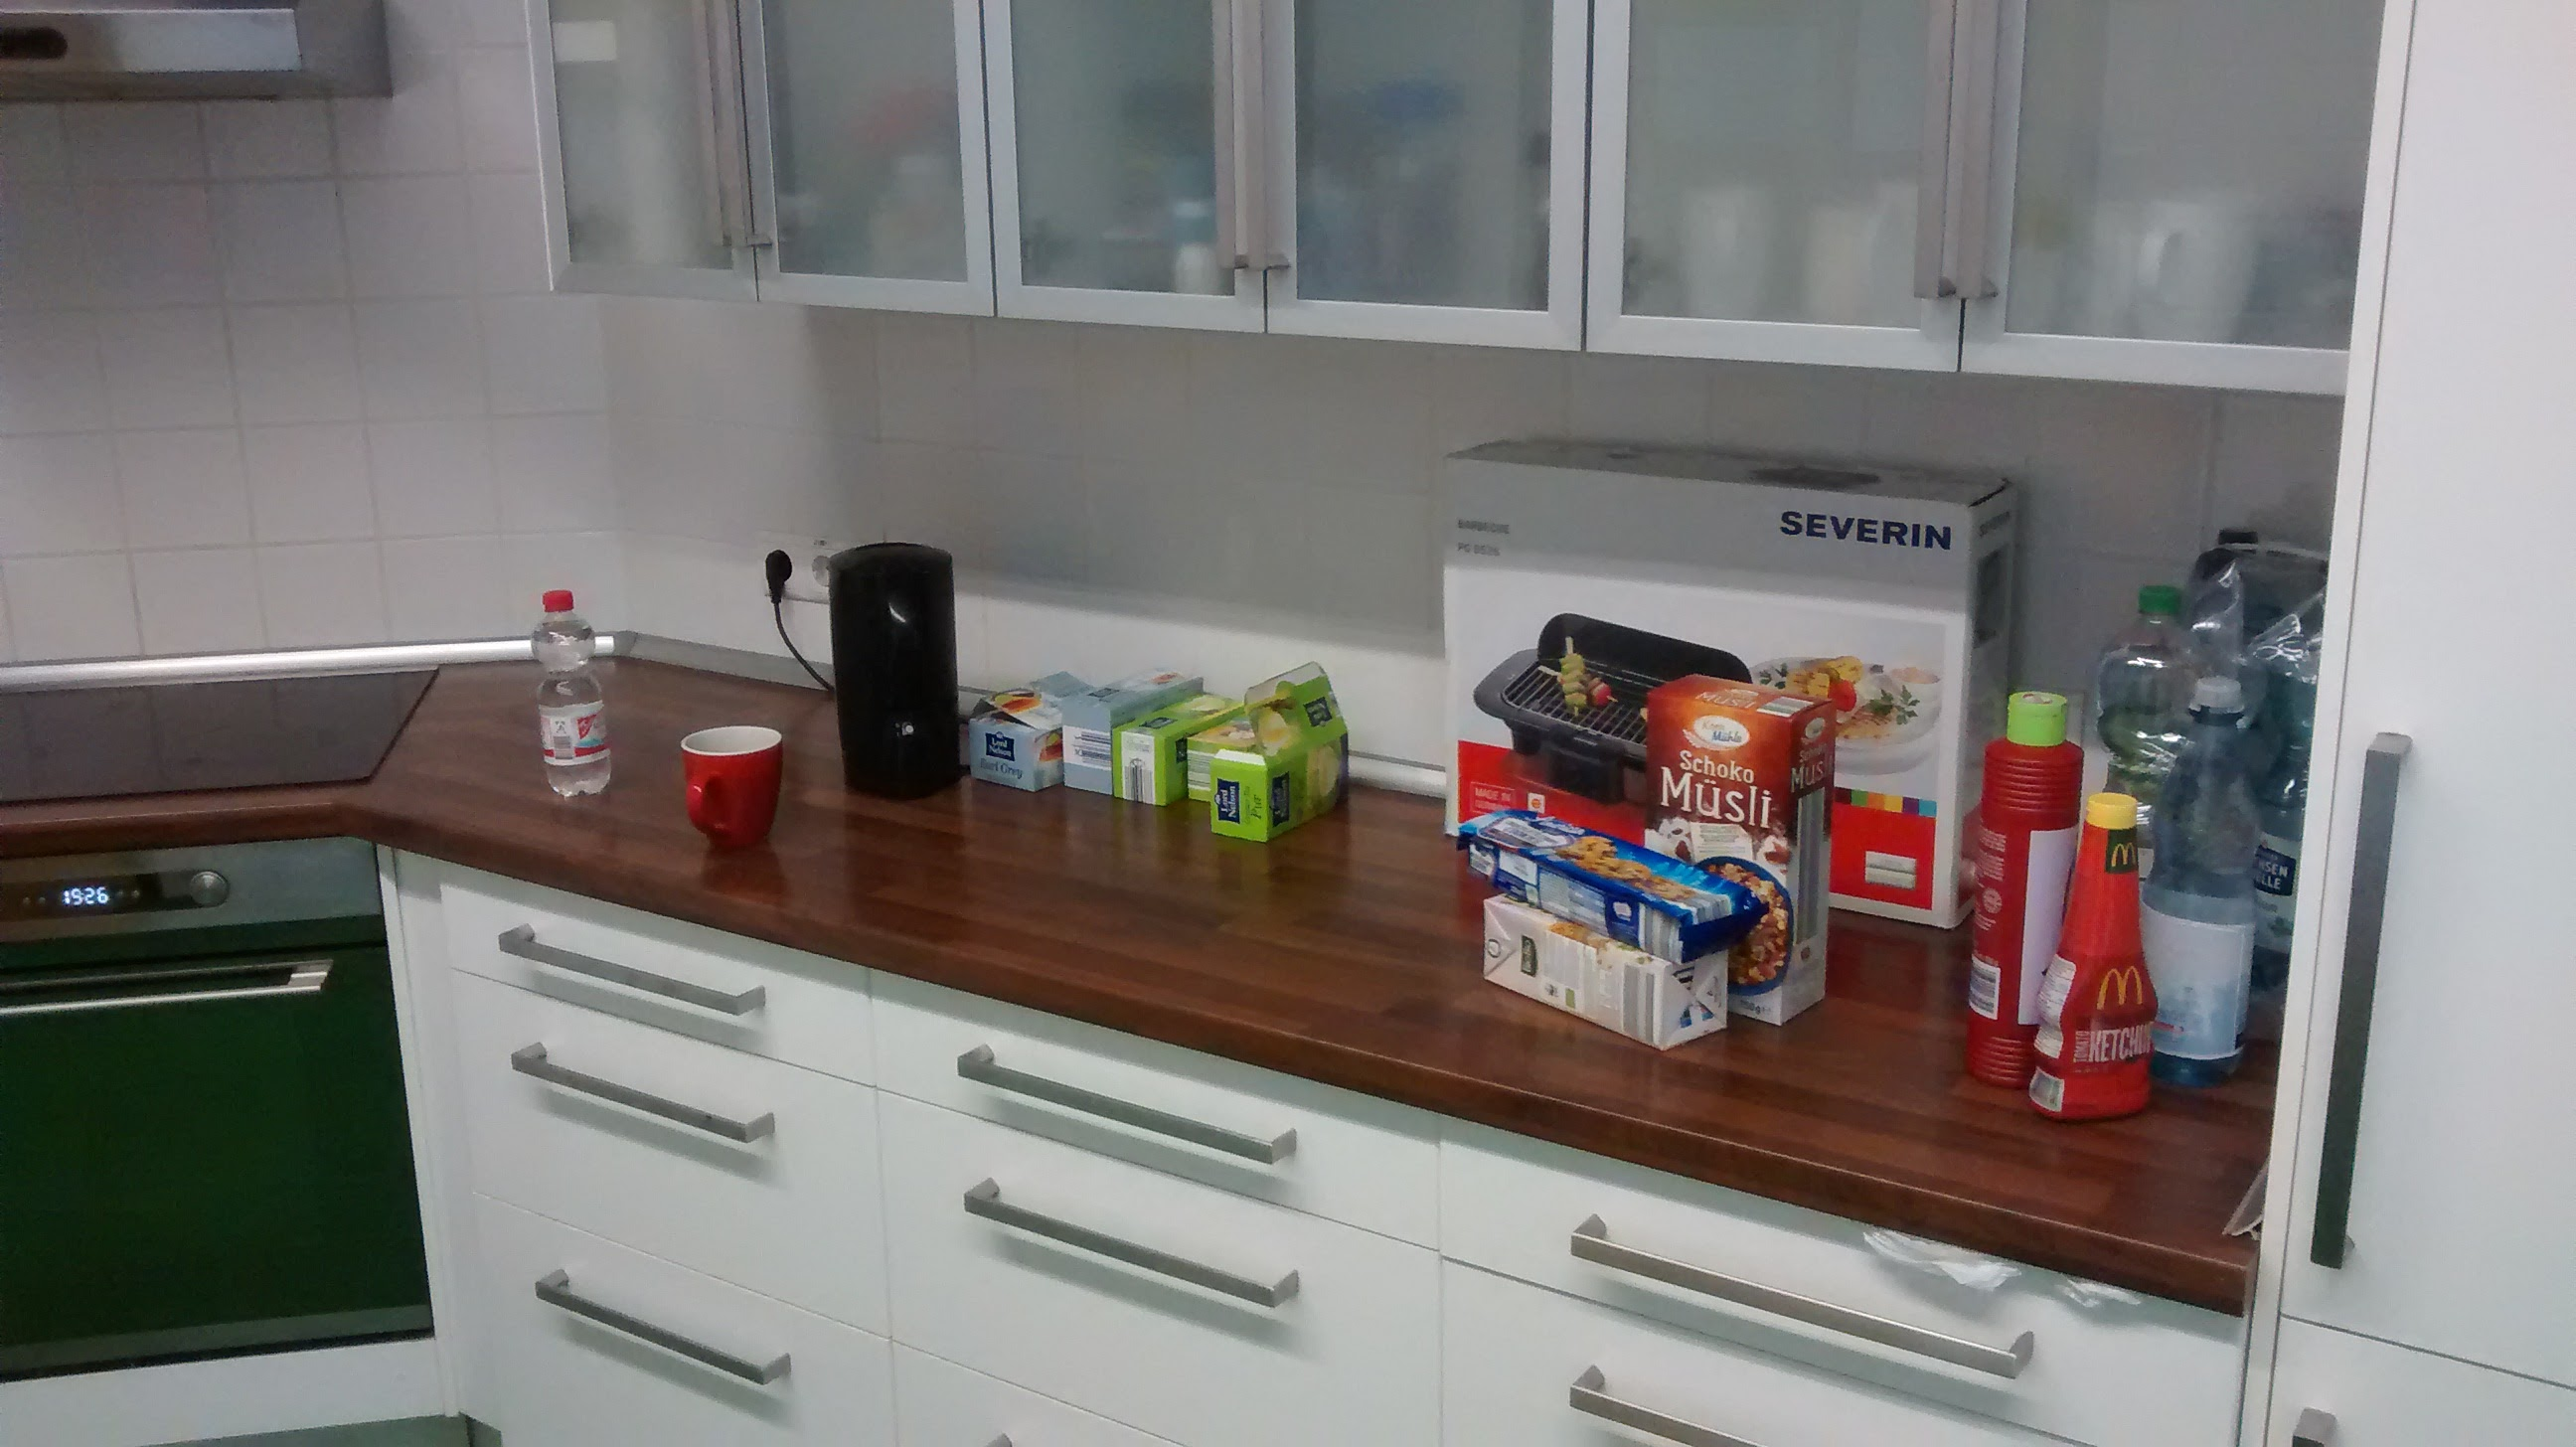
\includegraphics[width=\textwidth]{images/counter-top.jpg}
        \caption{counter-top}
        \label{fig:counter-top}
    \end{subfigure}
    \caption{Different possible object locations}\label{fig:alllocations}
\end{figure}
\begin{figure}
    \centering
    \begin{subfigure}[b]{0.3\textwidth}
        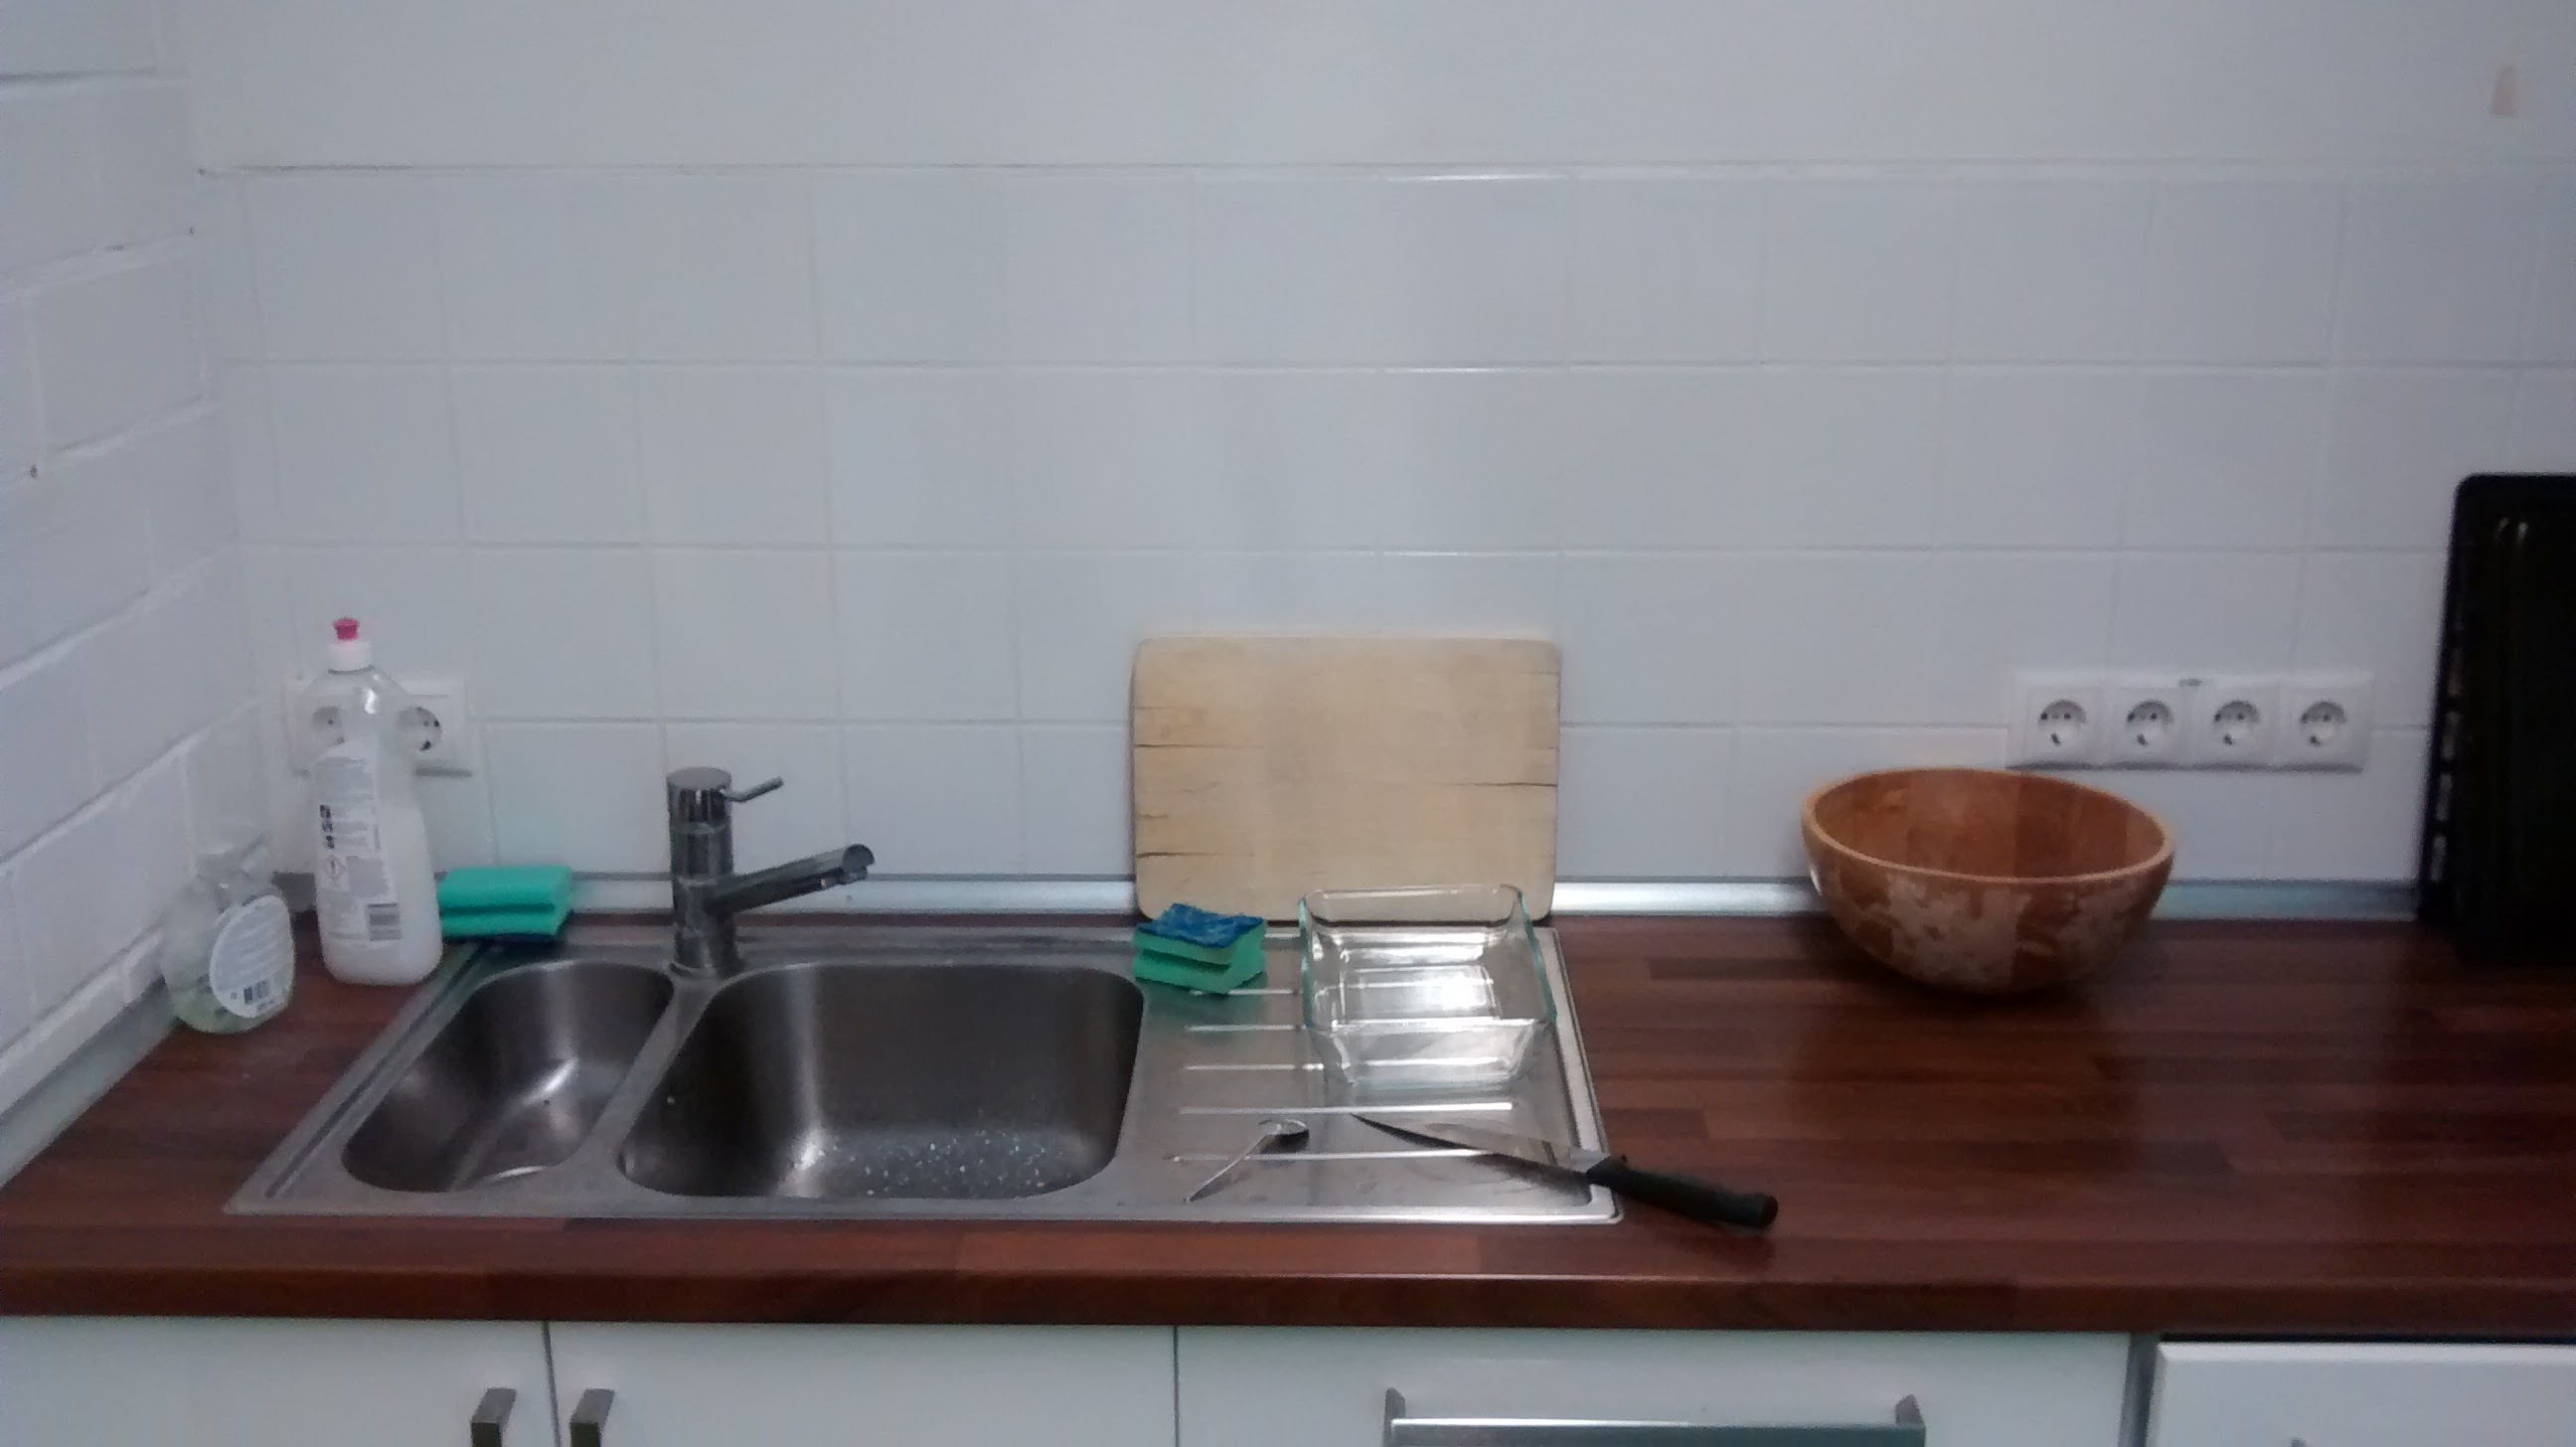
\includegraphics[width=\textwidth]{images/sink.jpg}
        \caption{Sink}
        \label{fig:sink}
    \end{subfigure}
    ~ %add desired spacing between images, e. g. ~, \quad, \qquad, \hfill etc. 
      %(or a blank line to force the subfigure onto a new line)
    \begin{subfigure}[b]{0.3\textwidth}
        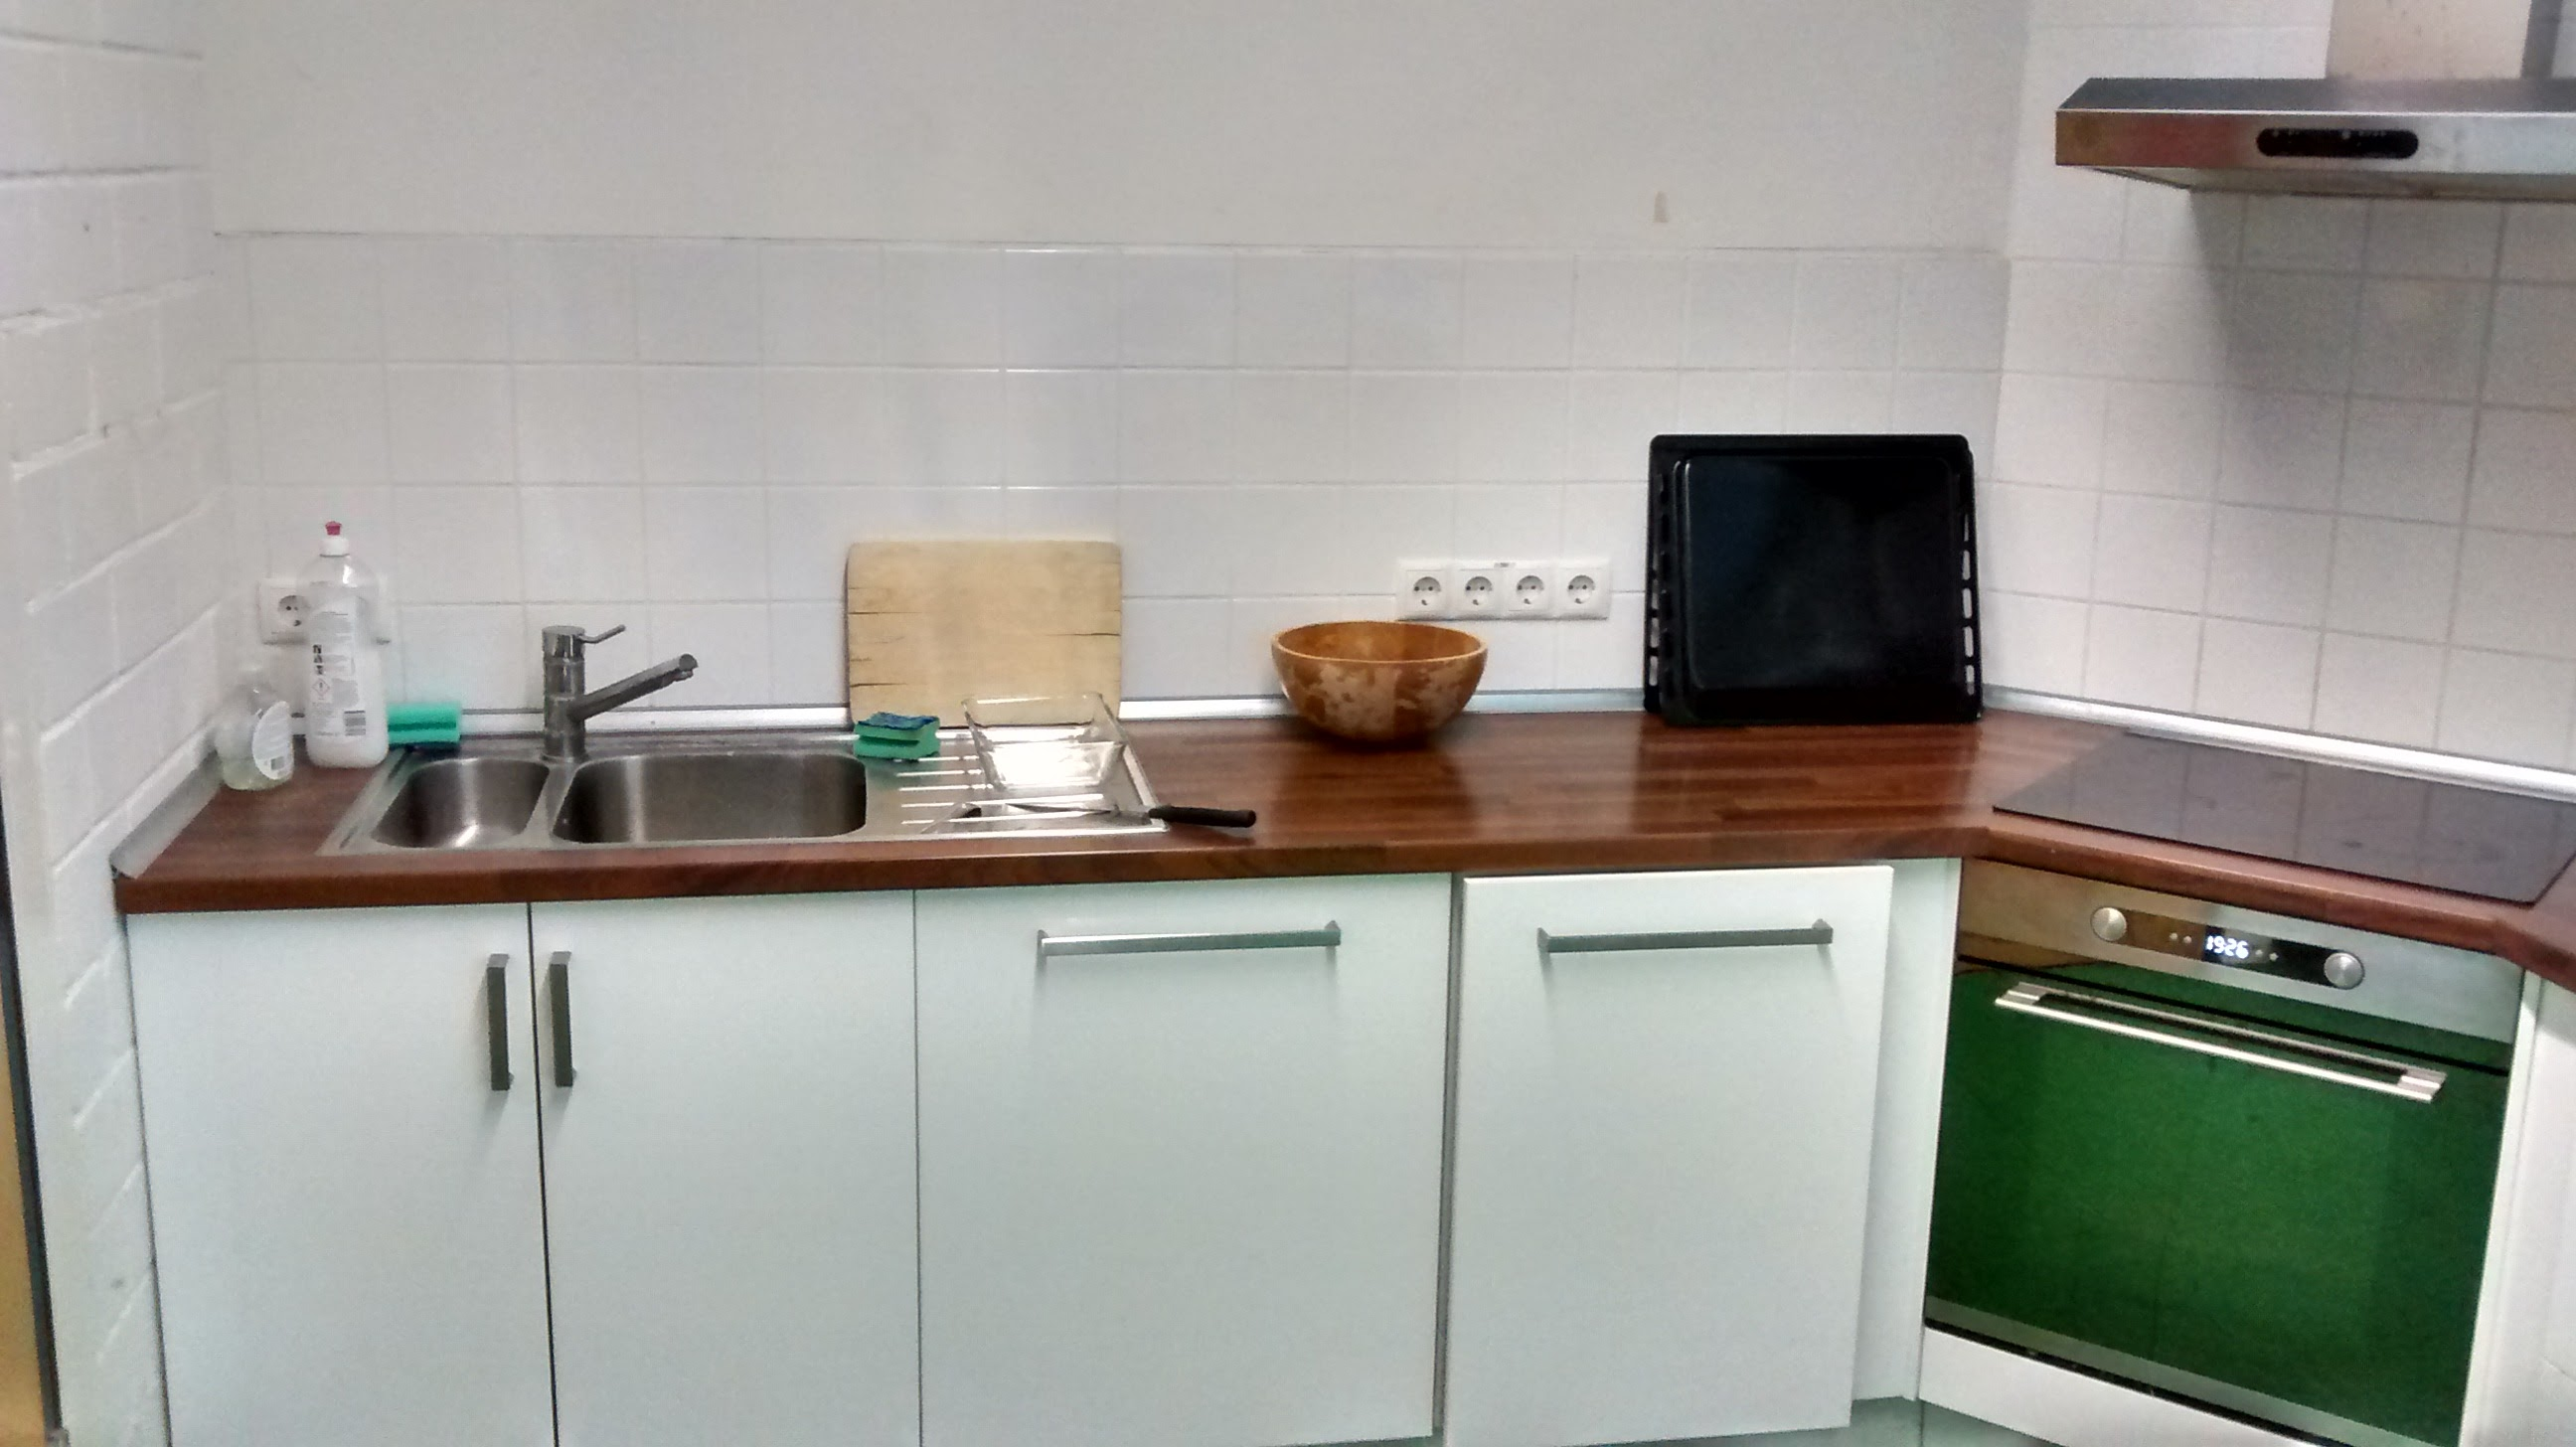
\includegraphics[width=\textwidth]{images/stove.jpg}
        \caption{Stove}
        \label{fig:stove}
    \end{subfigure}
    ~ %add desired spacing between images, e. g. ~, \quad, \qquad, \hfill etc. 
    %(or a blank line to force the subfigure onto a new line)
    \begin{subfigure}[b]{0.3\textwidth}
        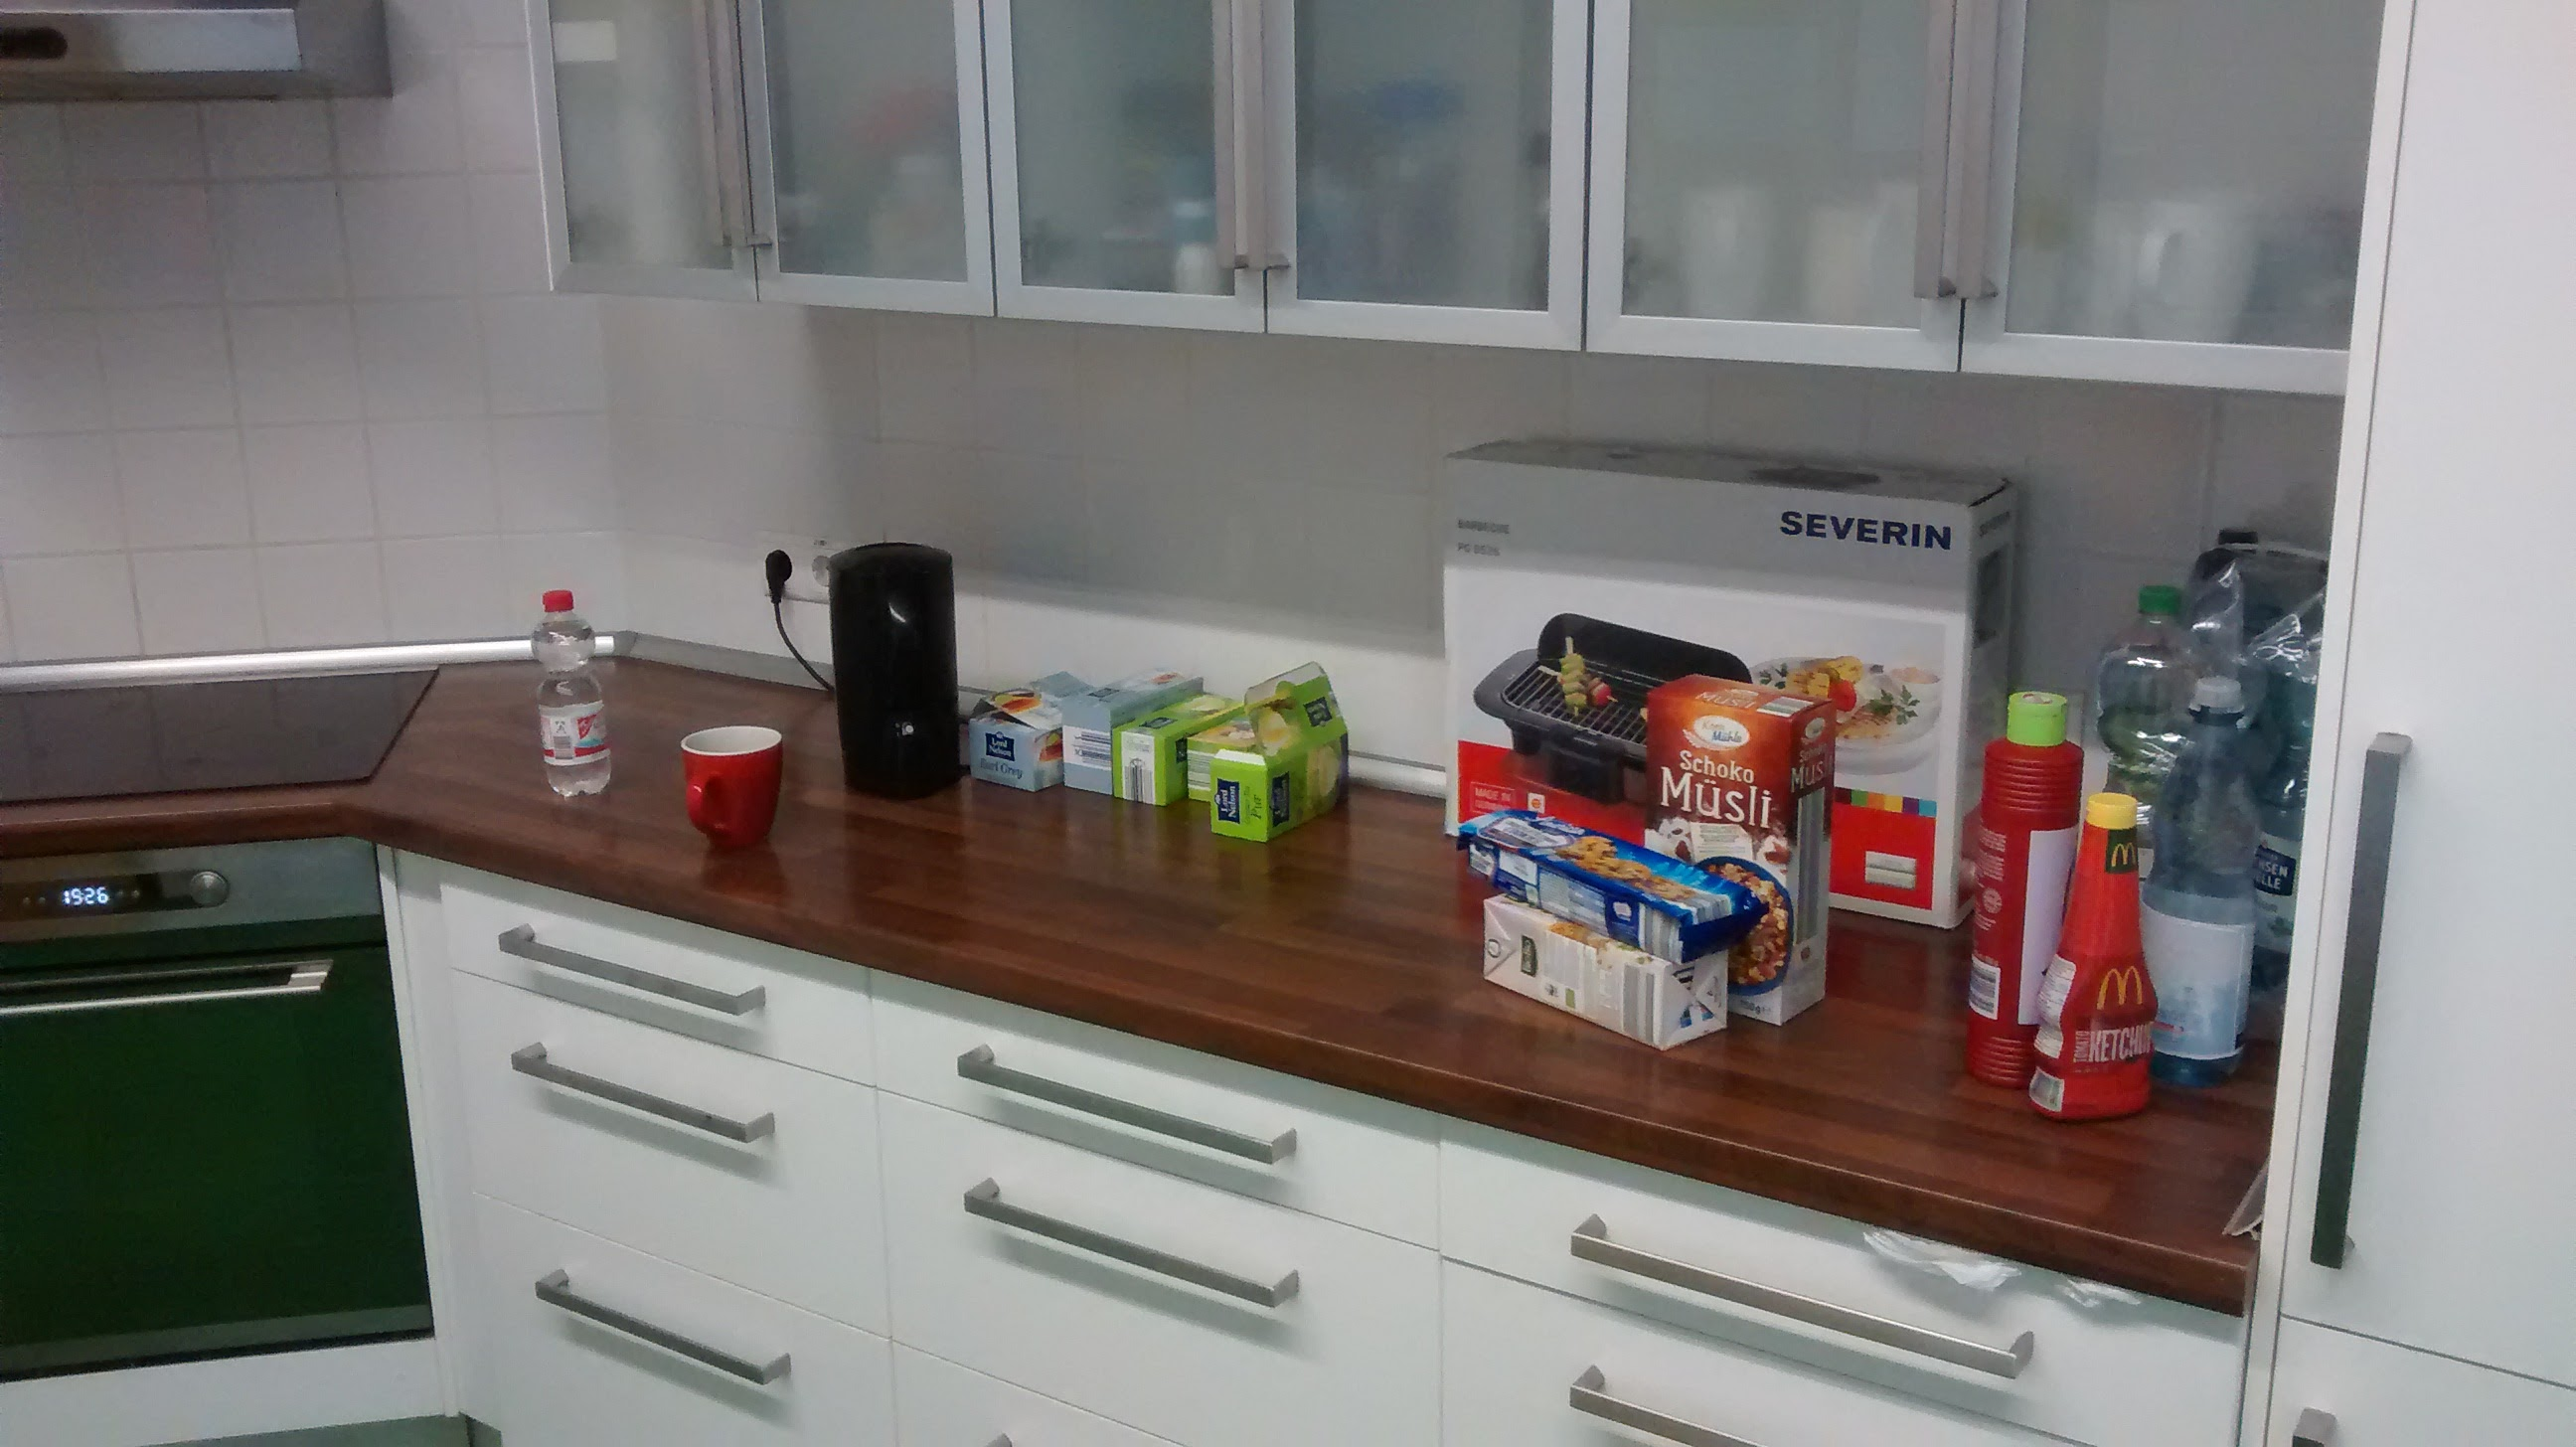
\includegraphics[width=\textwidth]{images/counter-top.jpg}
        \caption{counter-top}
        \label{fig:counter-top}
    \end{subfigure}
    \caption{Different possible object locations}\label{fig:alllocations}
\end{figure}
\begin{figure}
    \centering
    \begin{subfigure}[b]{0.3\textwidth}
        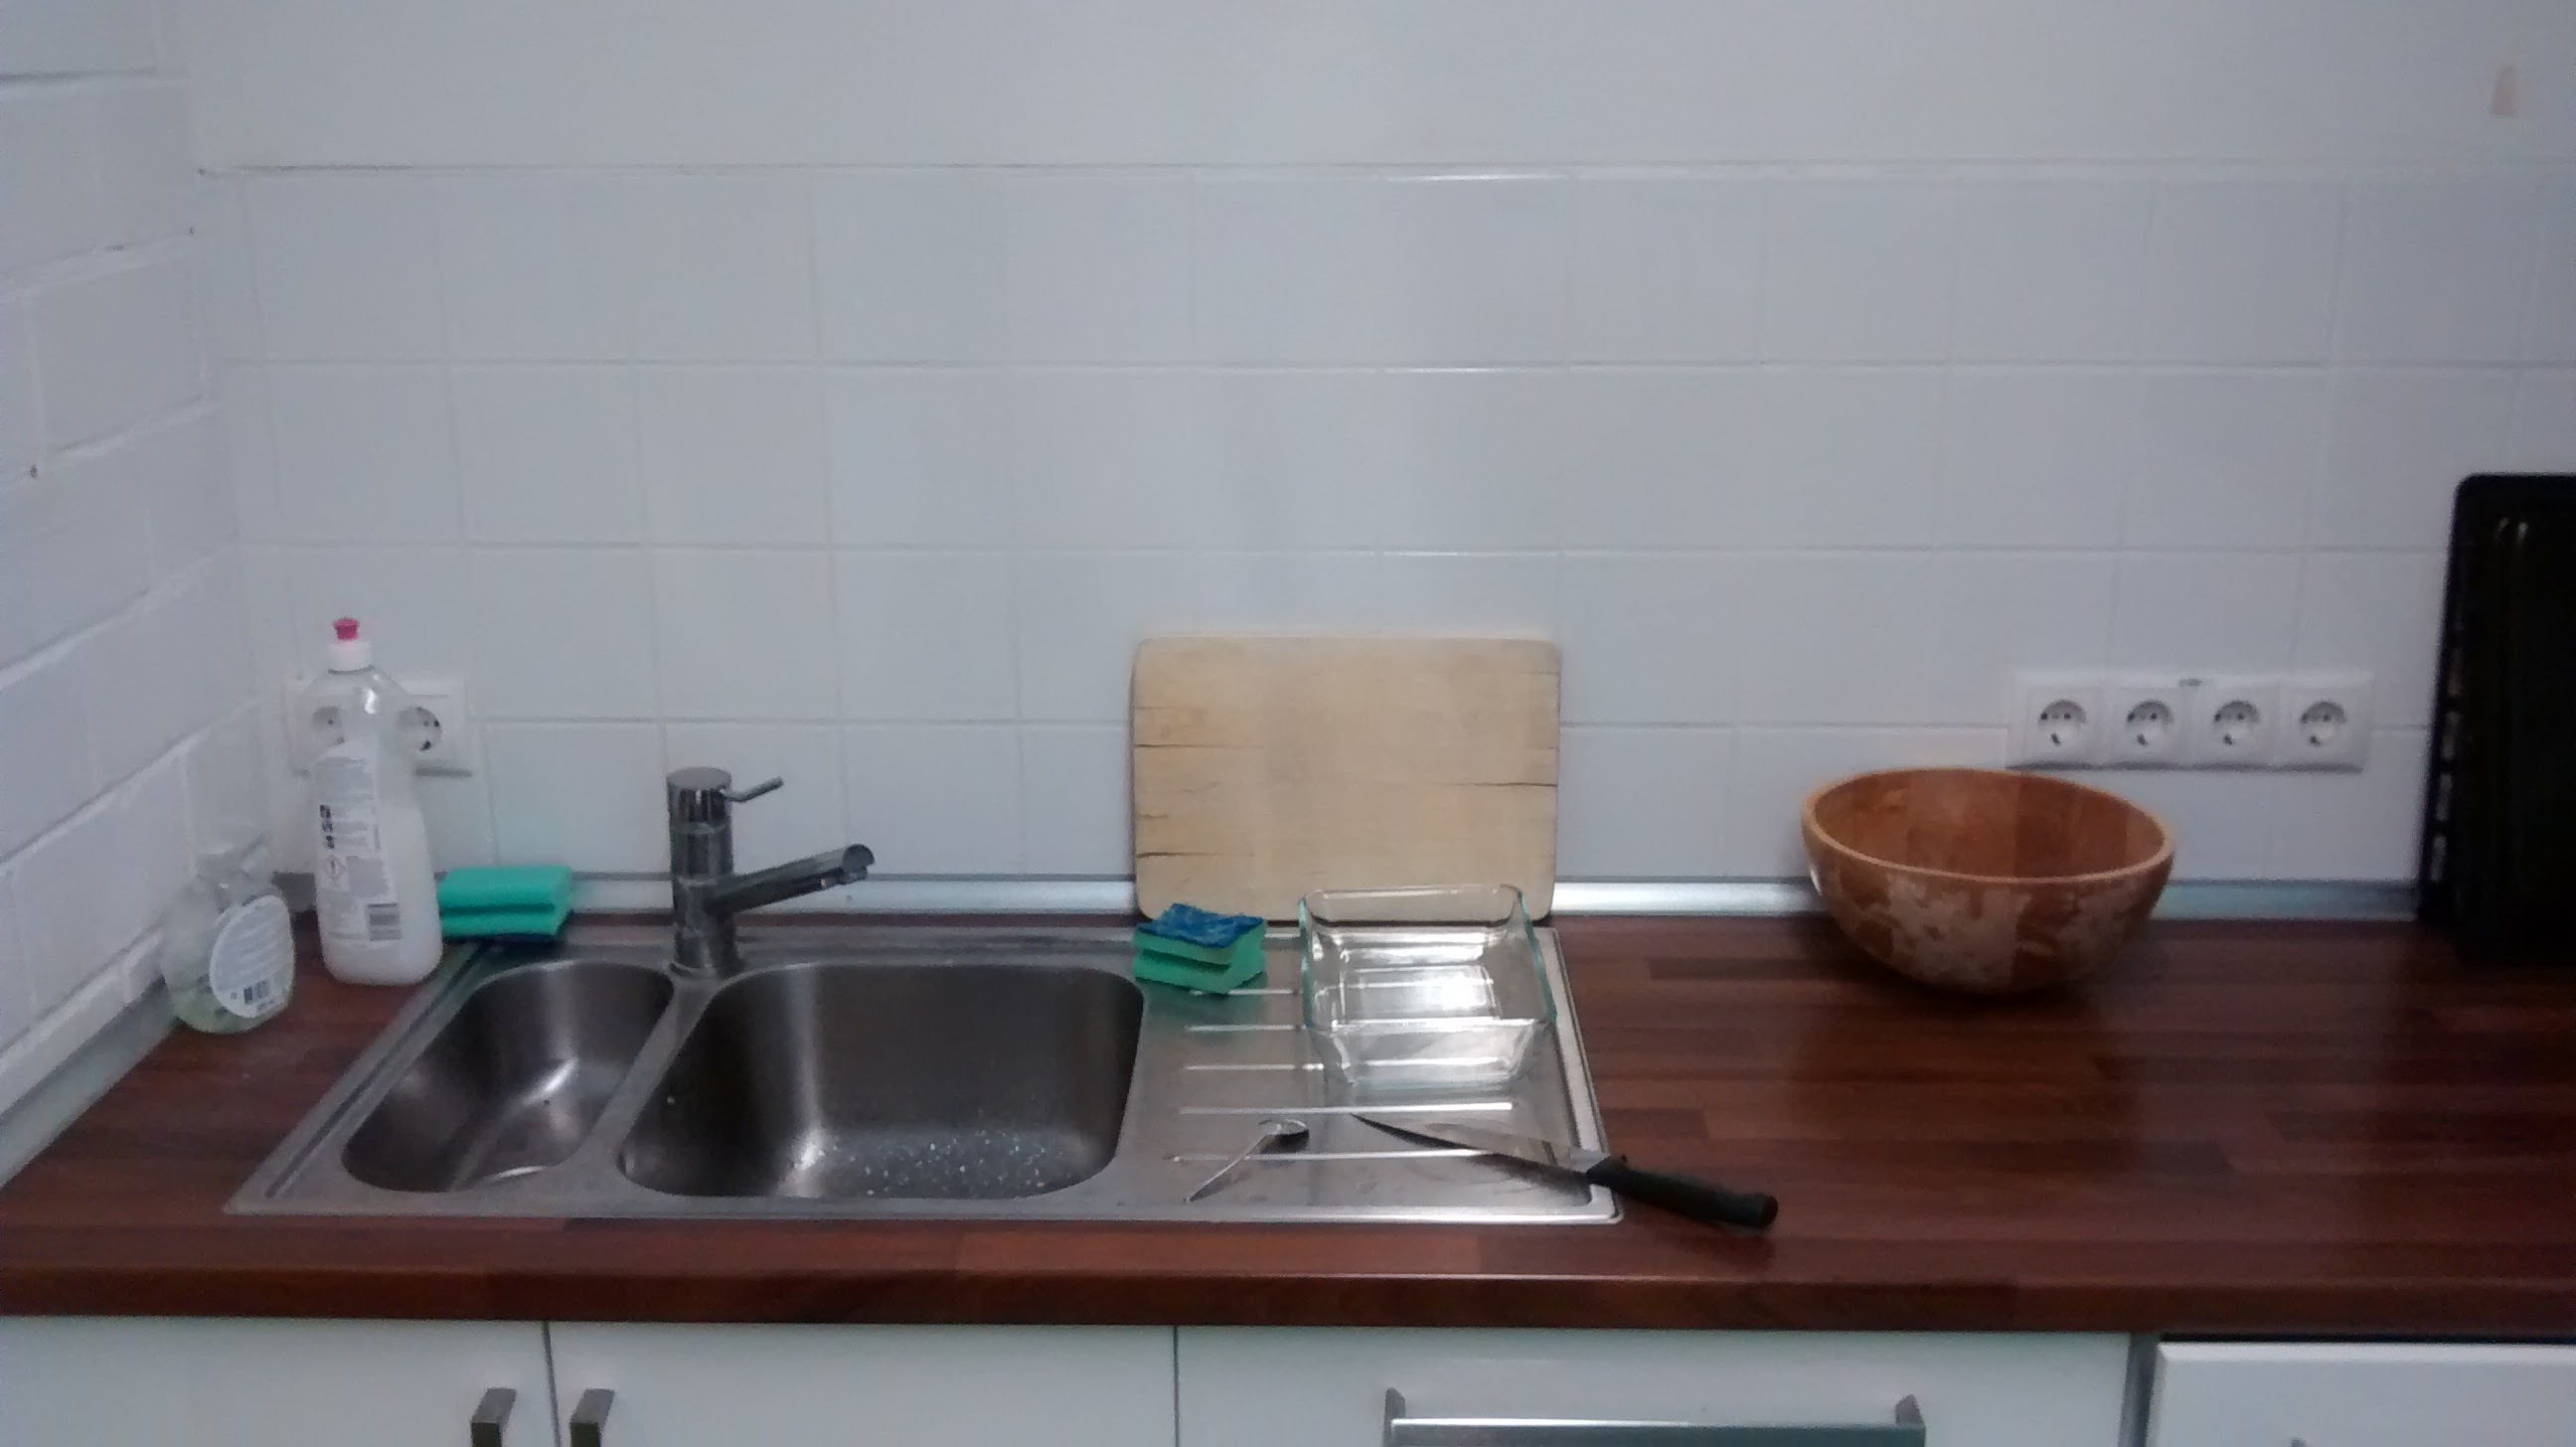
\includegraphics[width=\textwidth]{images/sink.jpg}
        \caption{Sink}
        \label{fig:sink}
    \end{subfigure}
    ~ %add desired spacing between images, e. g. ~, \quad, \qquad, \hfill etc. 
      %(or a blank line to force the subfigure onto a new line)
    \begin{subfigure}[b]{0.3\textwidth}
        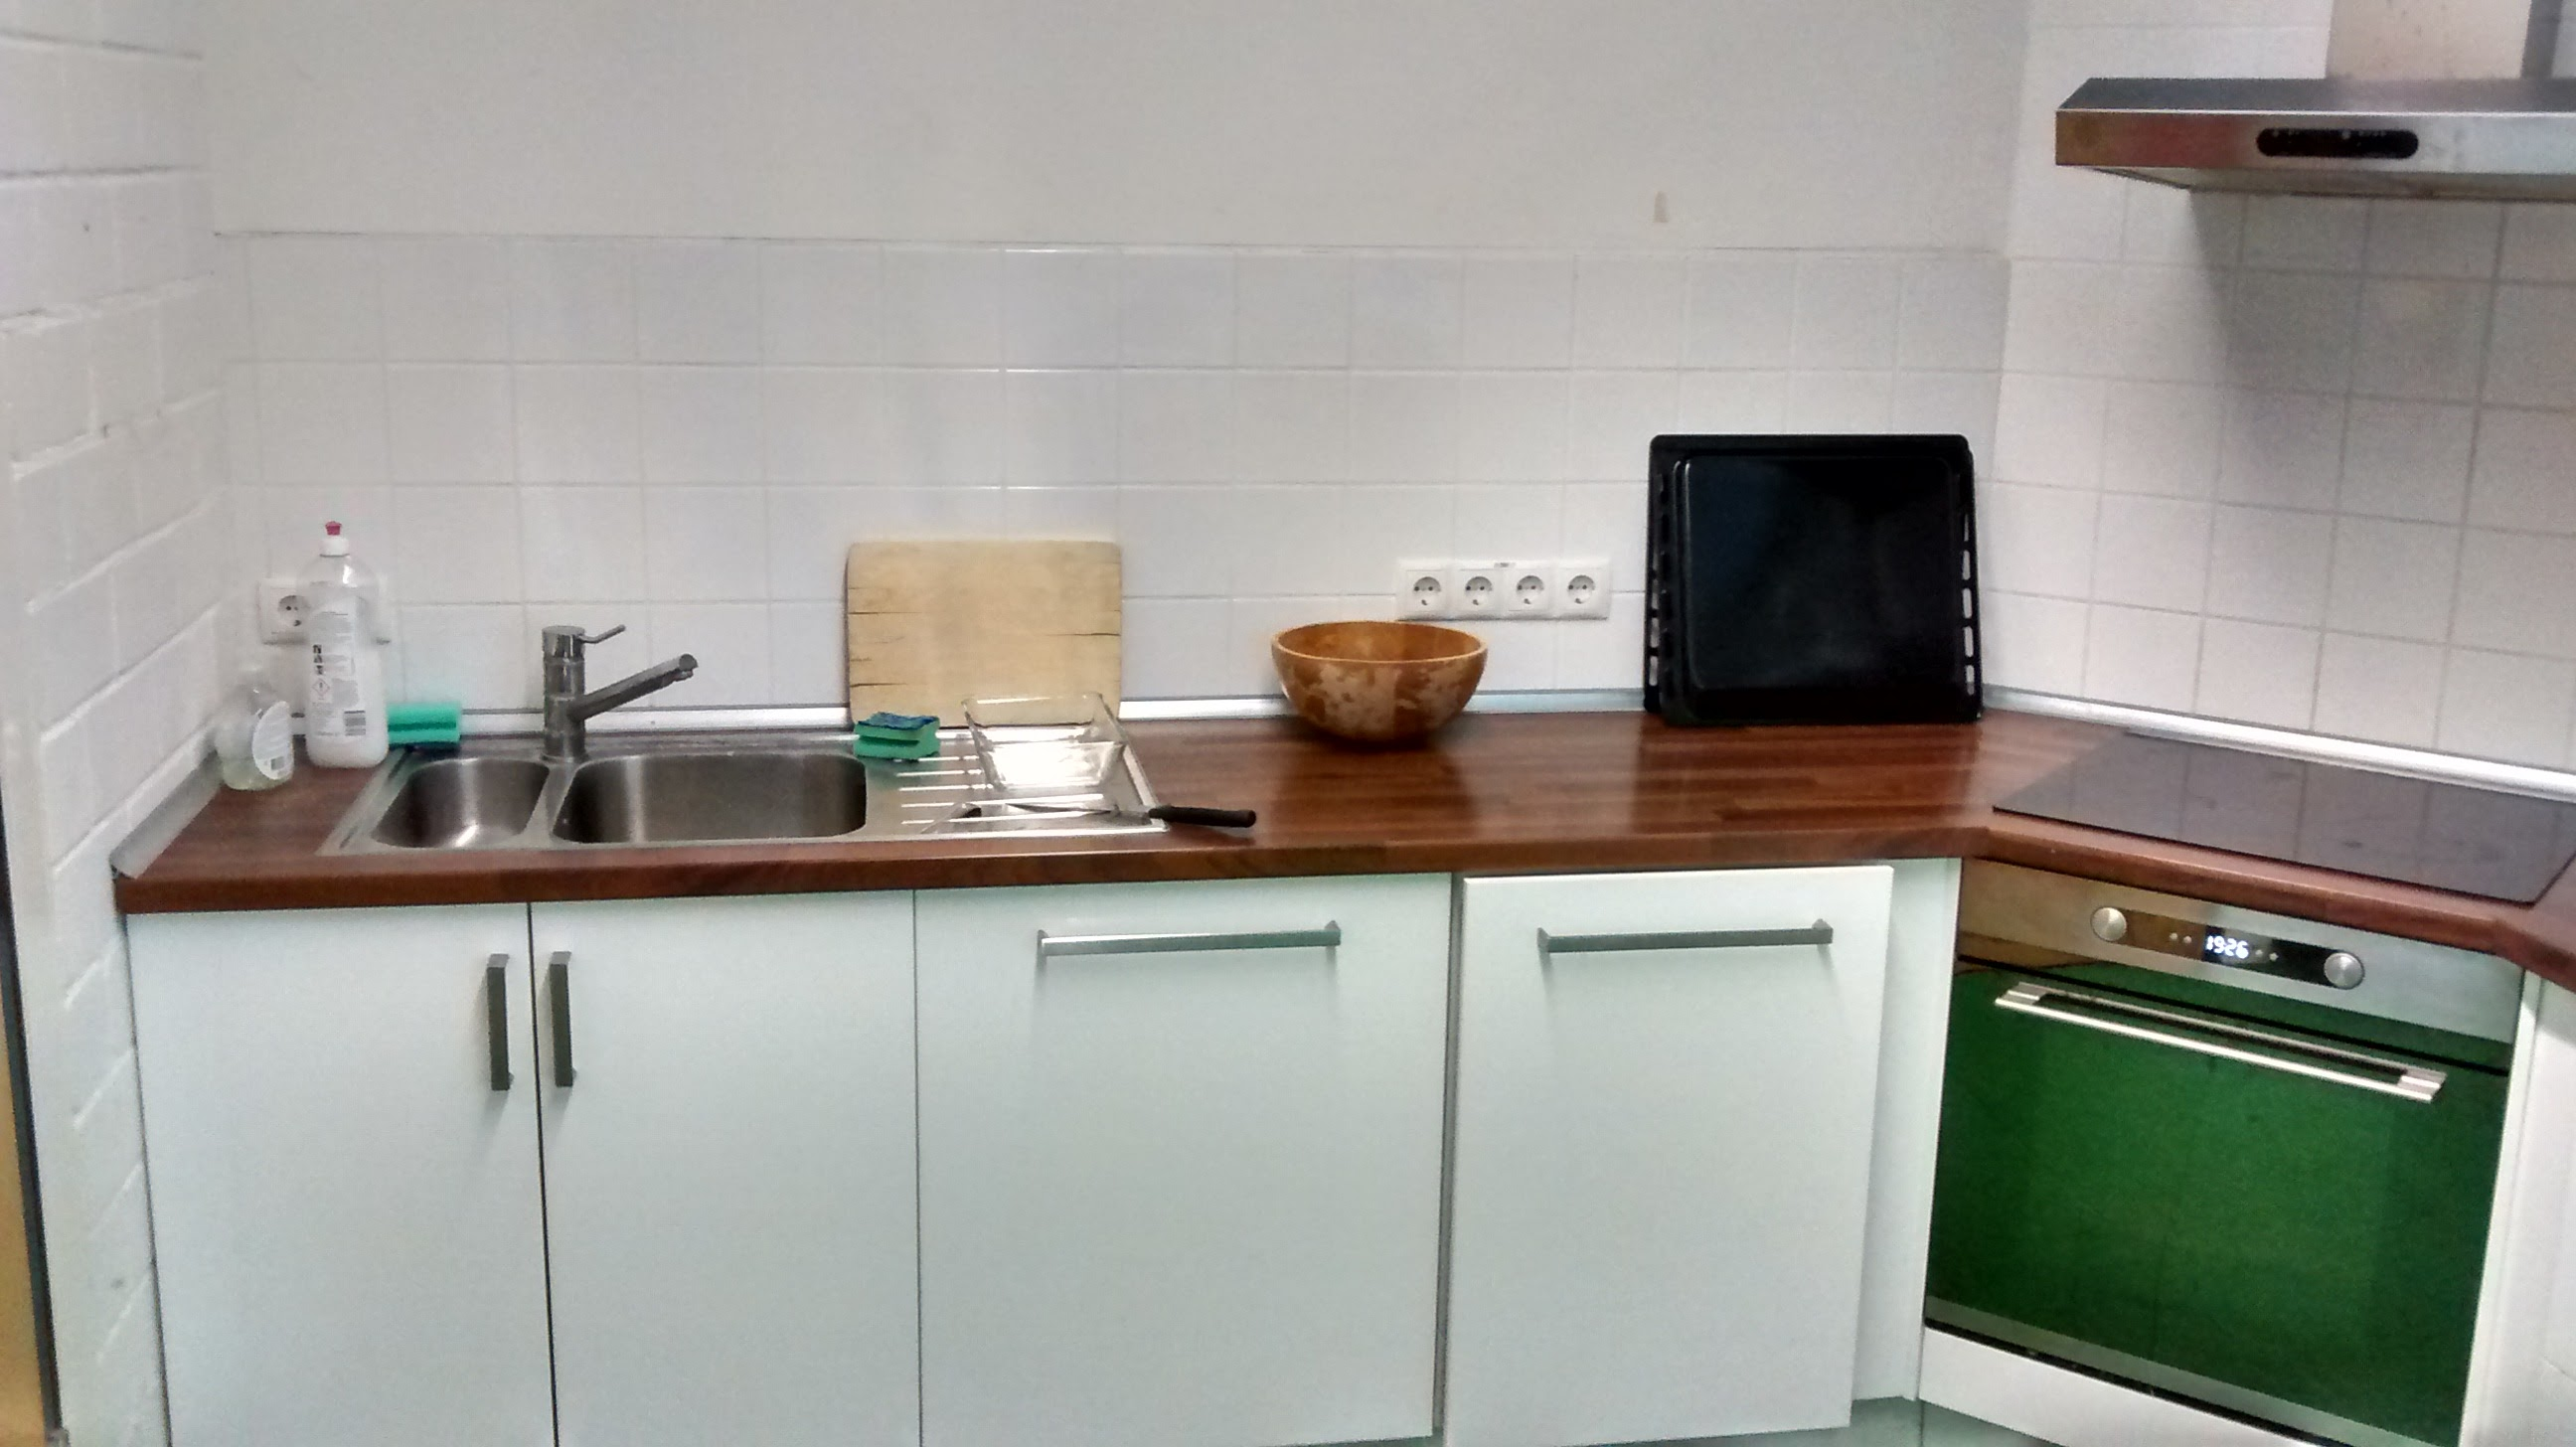
\includegraphics[width=\textwidth]{images/stove.jpg}
        \caption{Stove}
        \label{fig:stove}
    \end{subfigure}
    ~ %add desired spacing between images, e. g. ~, \quad, \qquad, \hfill etc. 
    %(or a blank line to force the subfigure onto a new line)
    \begin{subfigure}[b]{0.3\textwidth}
        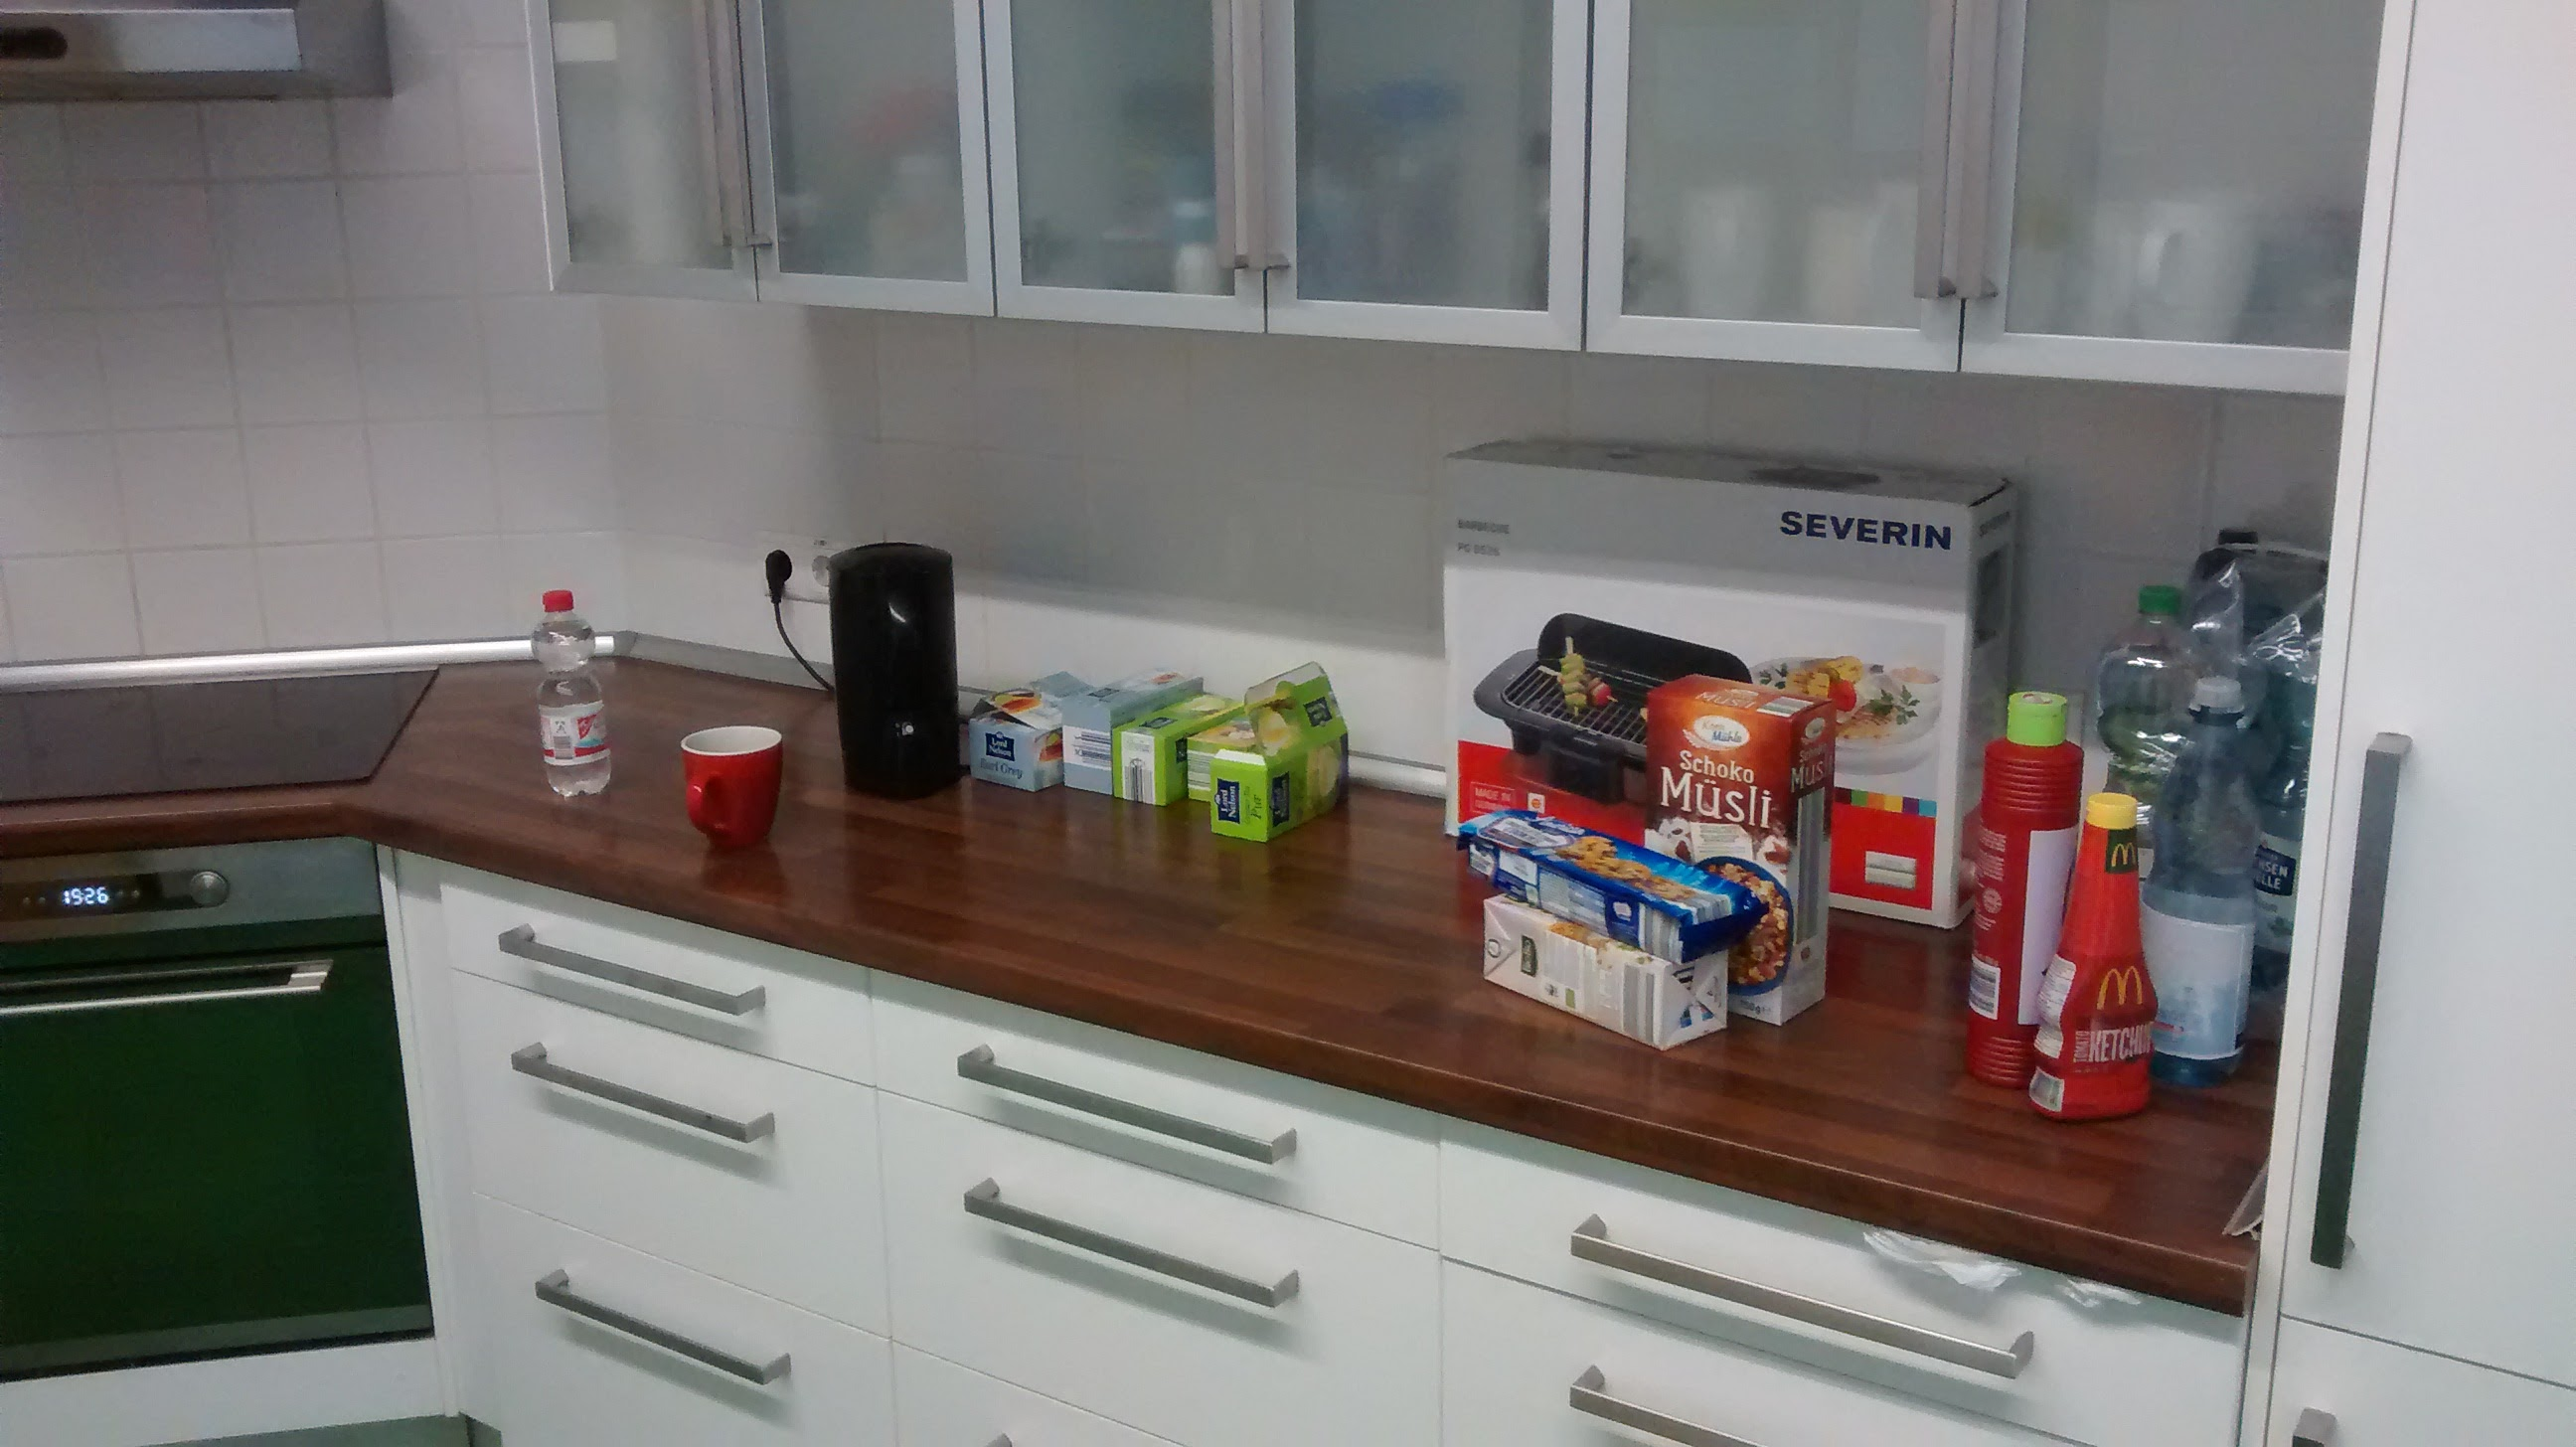
\includegraphics[width=\textwidth]{images/counter-top.jpg}
        \caption{counter-top}
        \label{fig:counter-top}
    \end{subfigure}
    \caption{Different possible object locations}\label{fig:alllocations}
\end{figure}
\begin{figure}
    \centering
    \begin{subfigure}[b]{0.3\textwidth}
        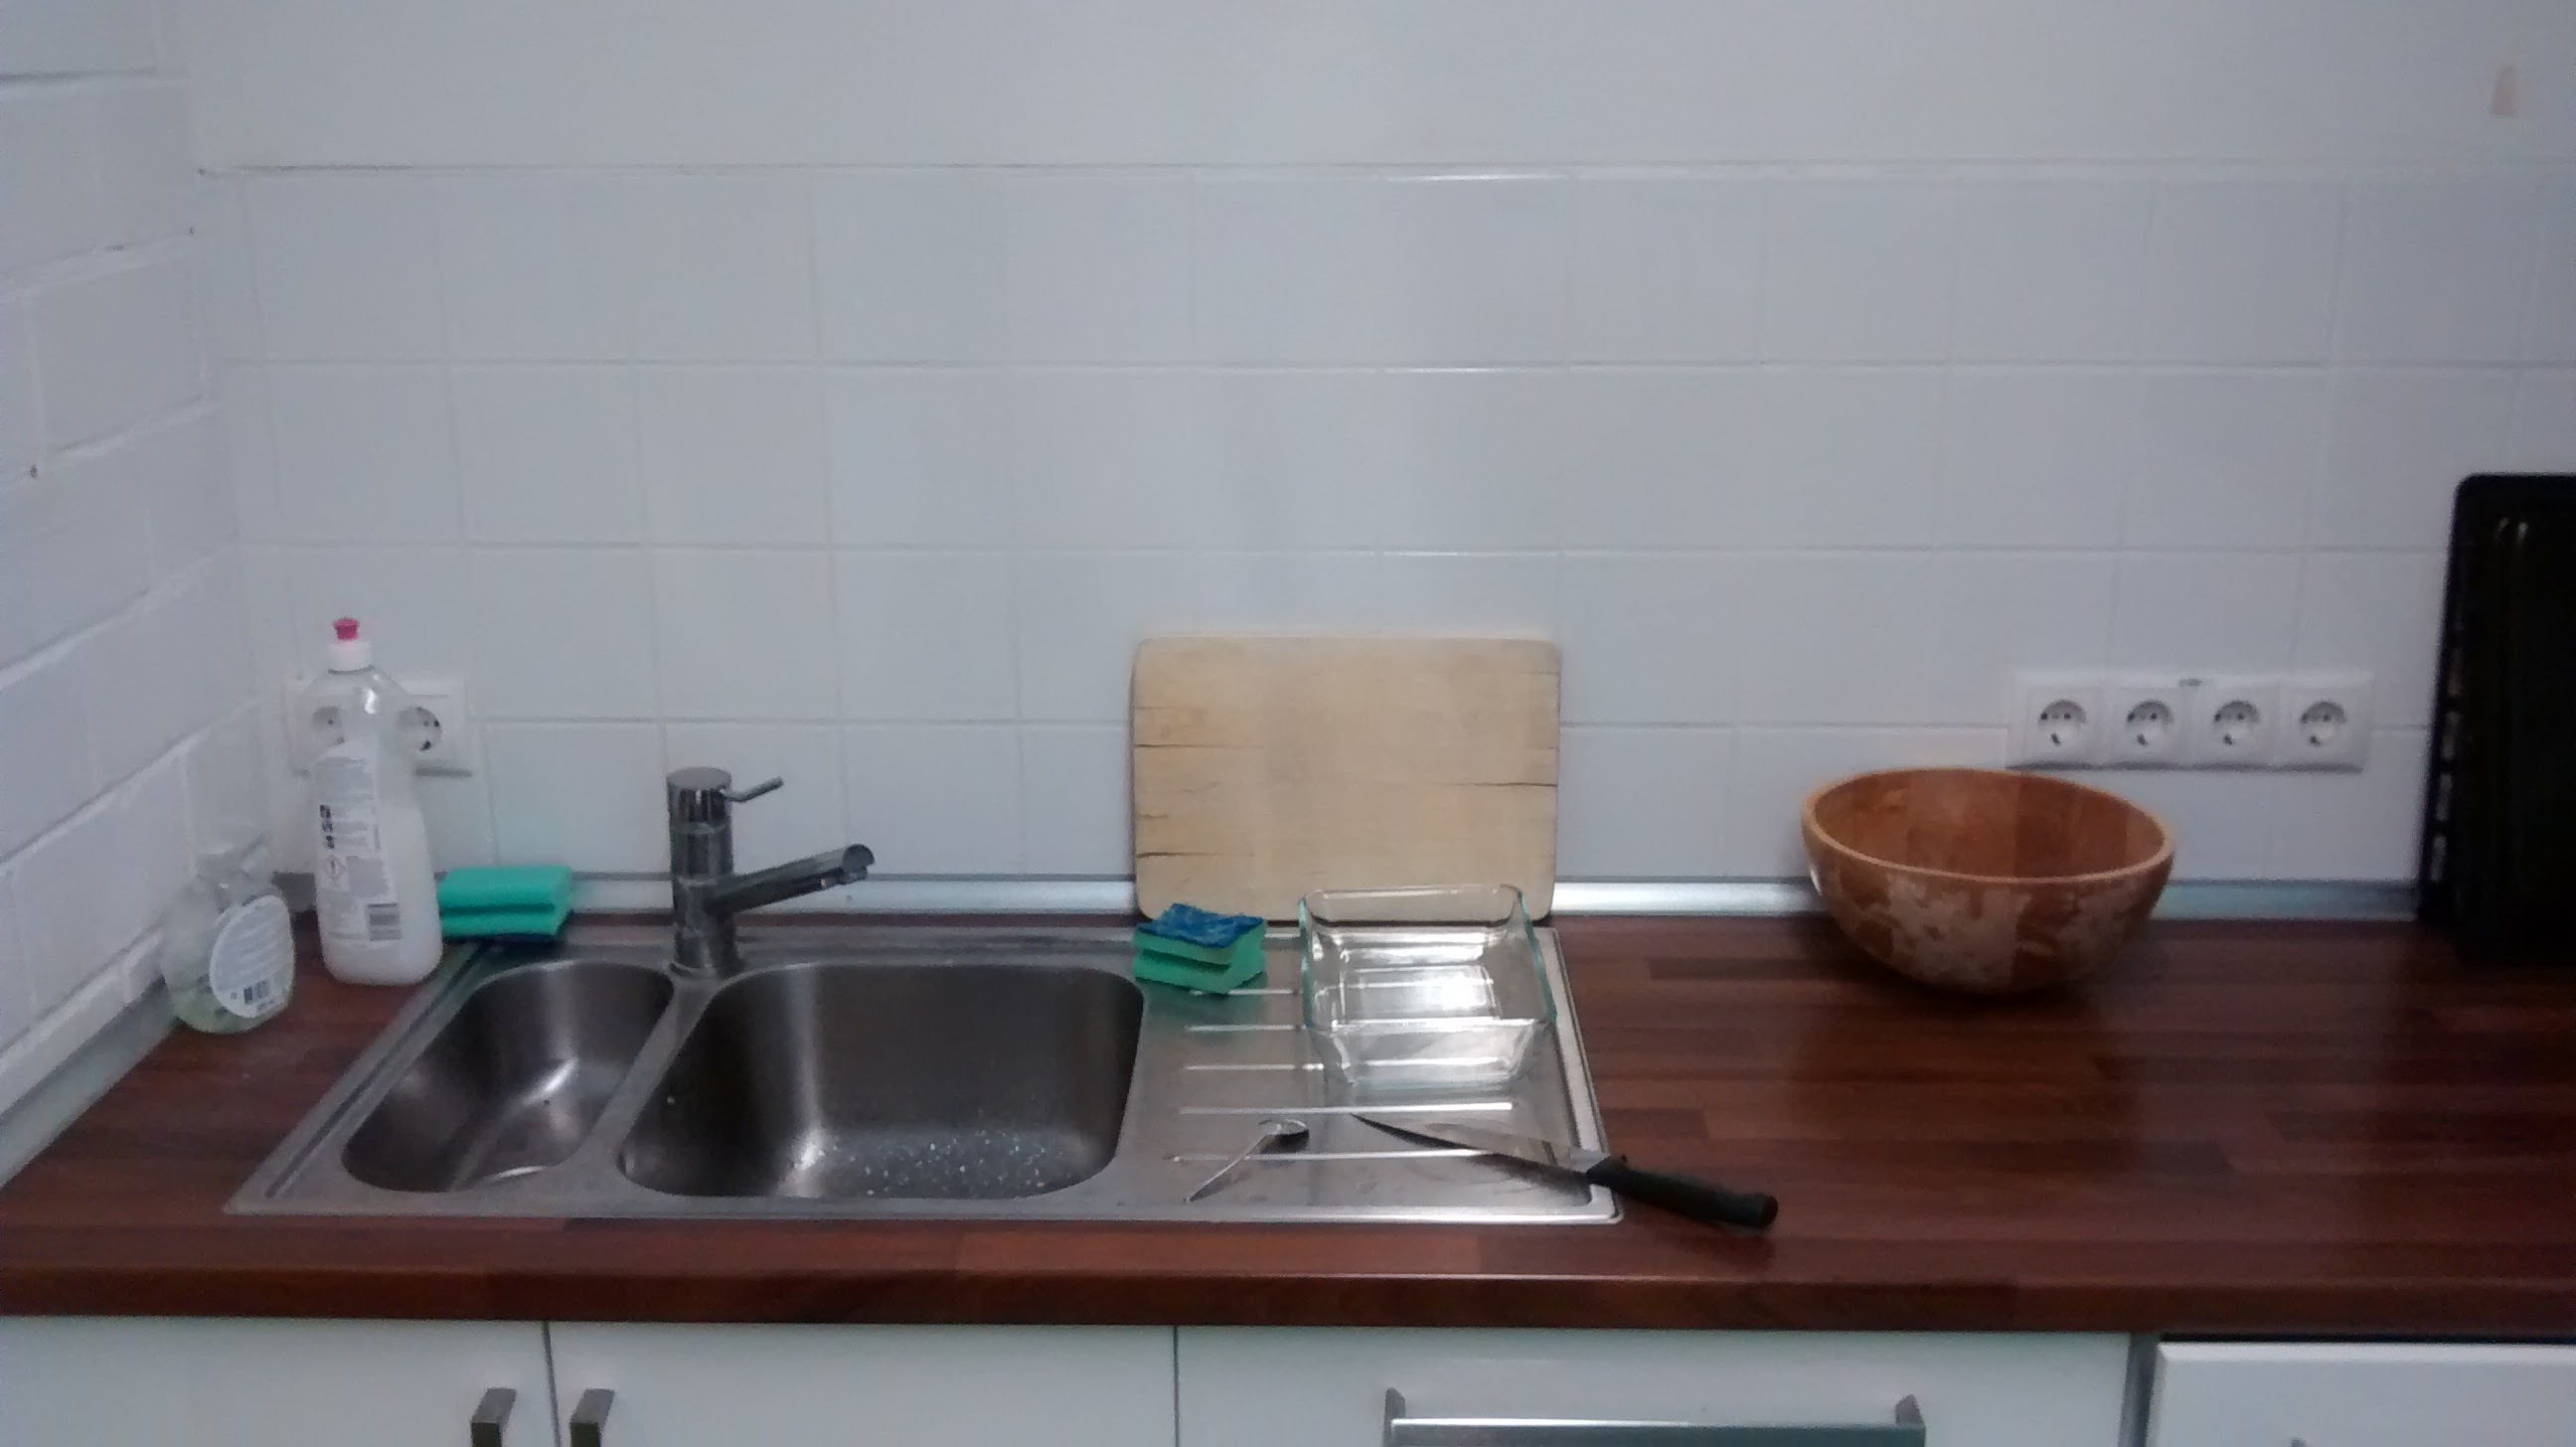
\includegraphics[width=\textwidth]{images/sink.jpg}
        \caption{Sink}
        \label{fig:sink}
    \end{subfigure}
    ~ %add desired spacing between images, e. g. ~, \quad, \qquad, \hfill etc. 
      %(or a blank line to force the subfigure onto a new line)
    \begin{subfigure}[b]{0.3\textwidth}
        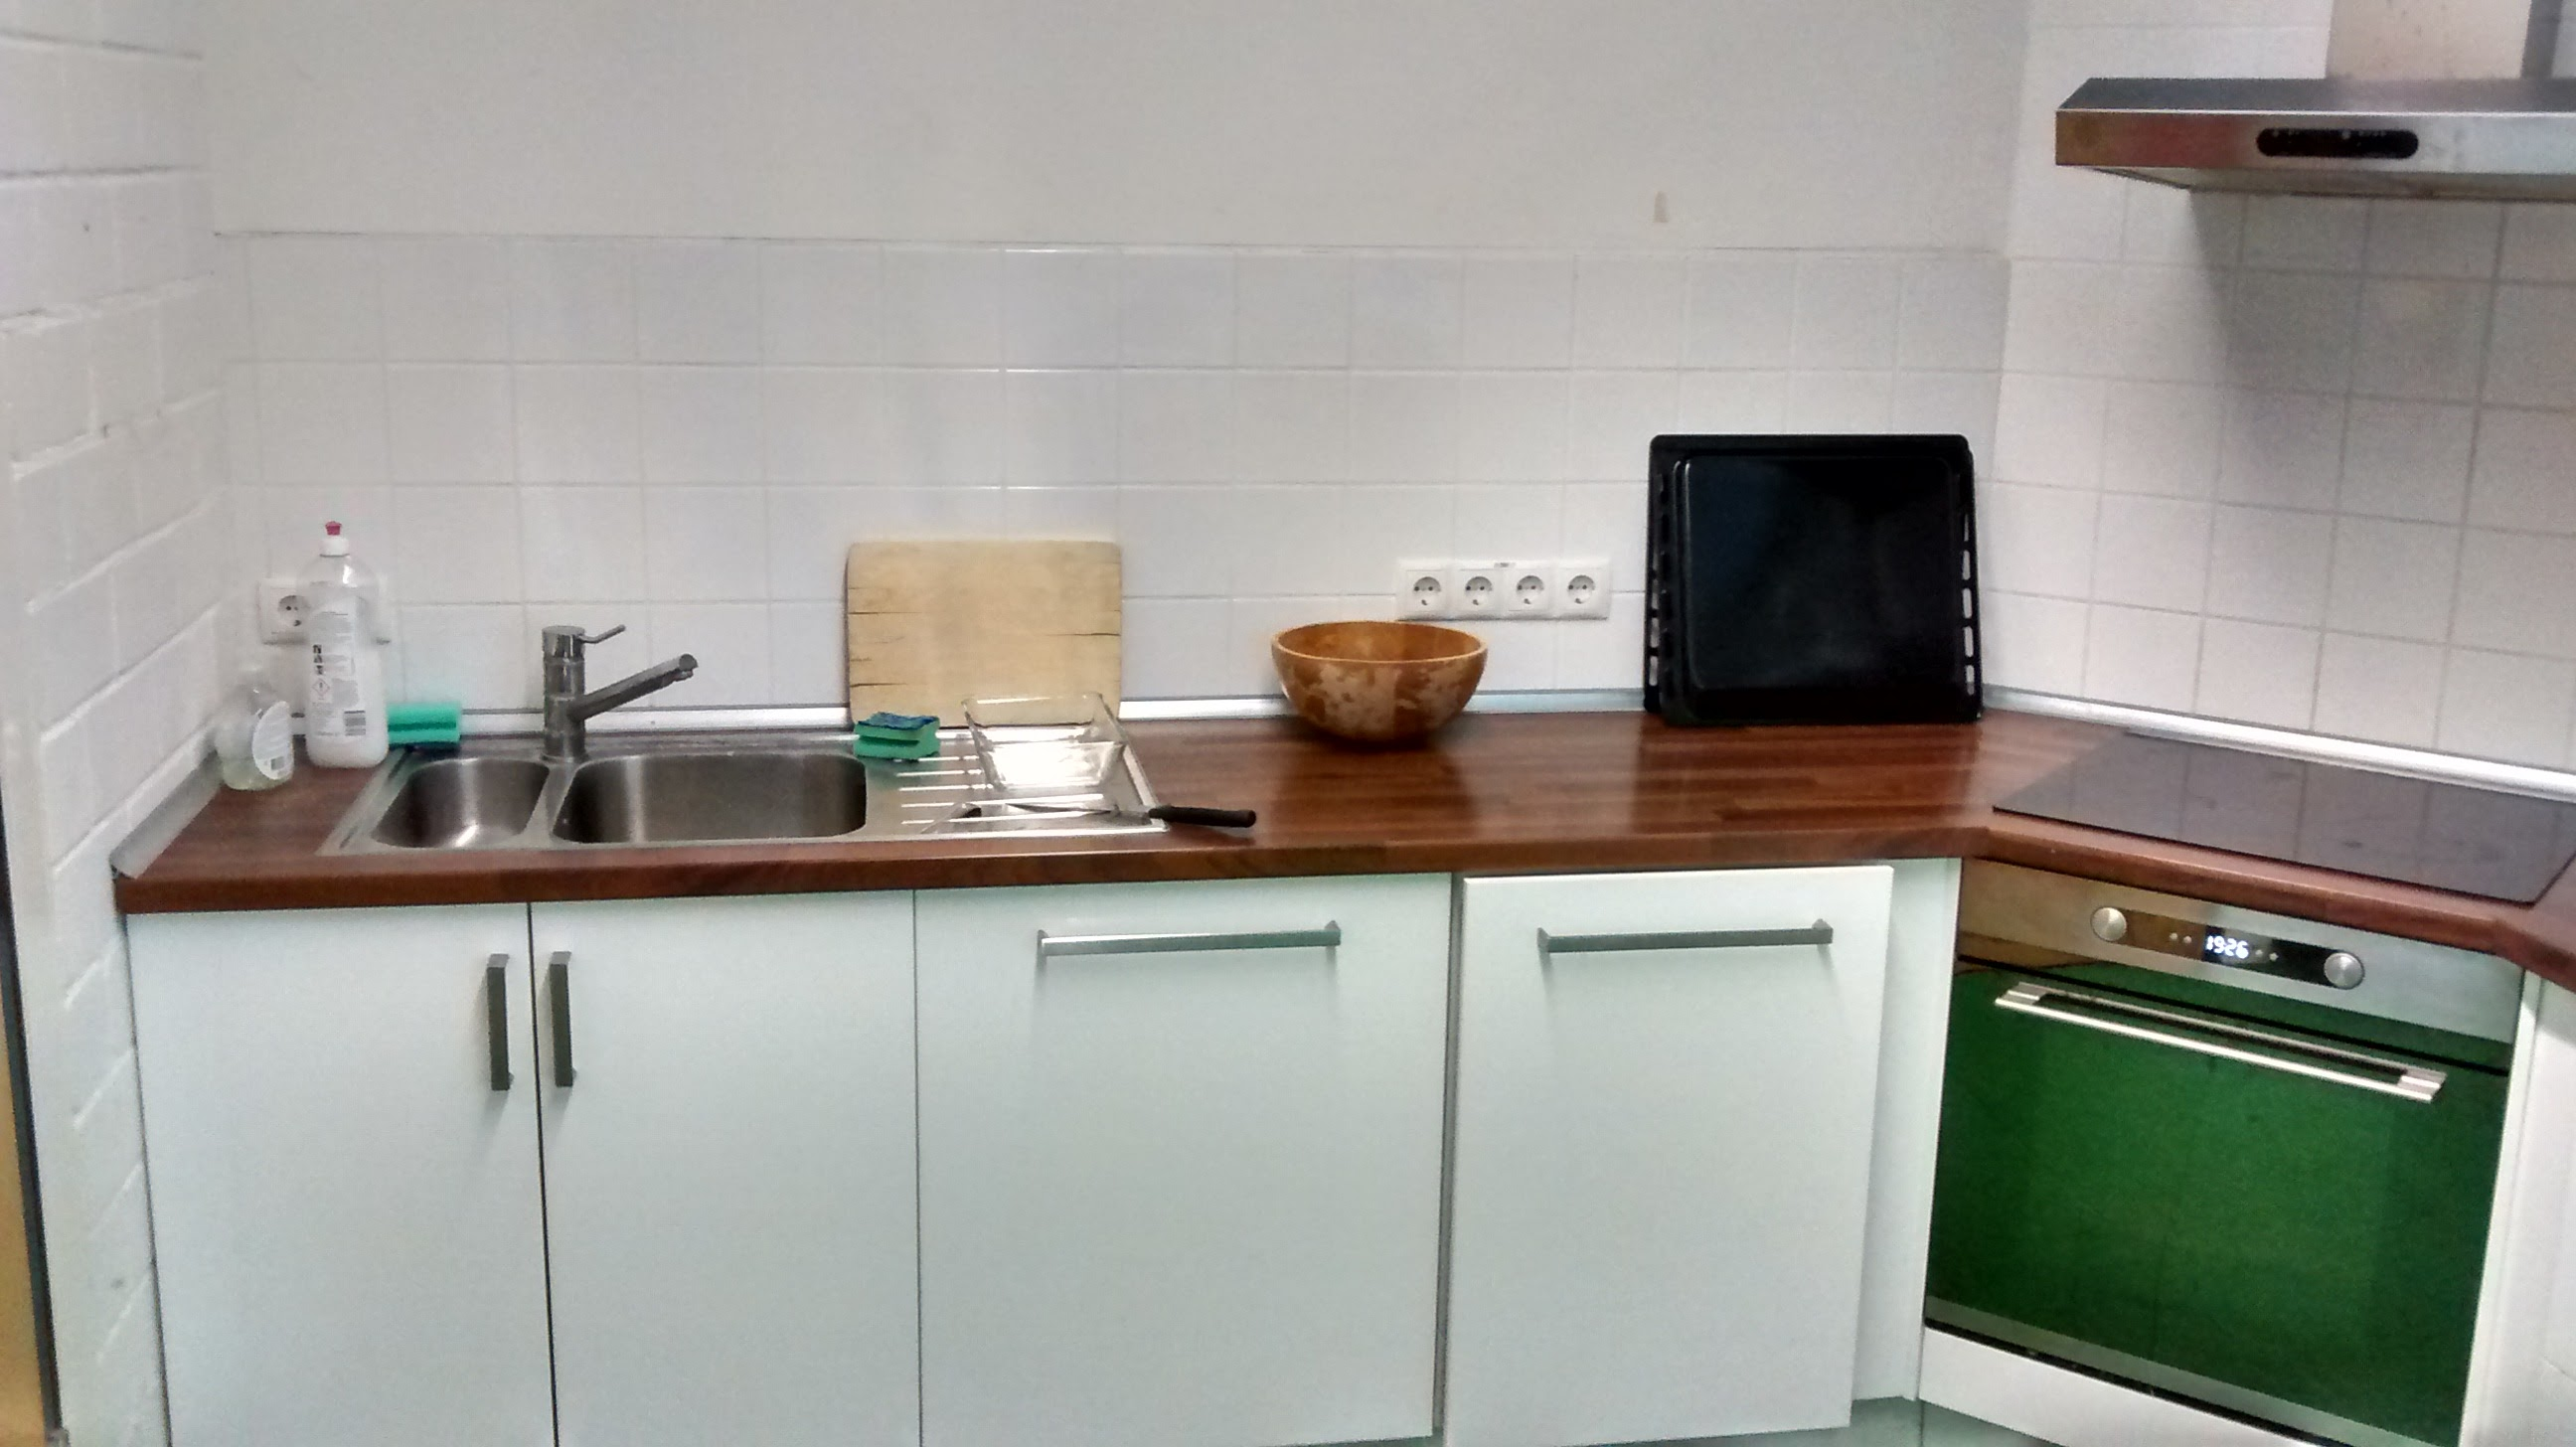
\includegraphics[width=\textwidth]{images/stove.jpg}
        \caption{Stove}
        \label{fig:stove}
    \end{subfigure}
    ~ %add desired spacing between images, e. g. ~, \quad, \qquad, \hfill etc. 
    %(or a blank line to force the subfigure onto a new line)
    \begin{subfigure}[b]{0.3\textwidth}
        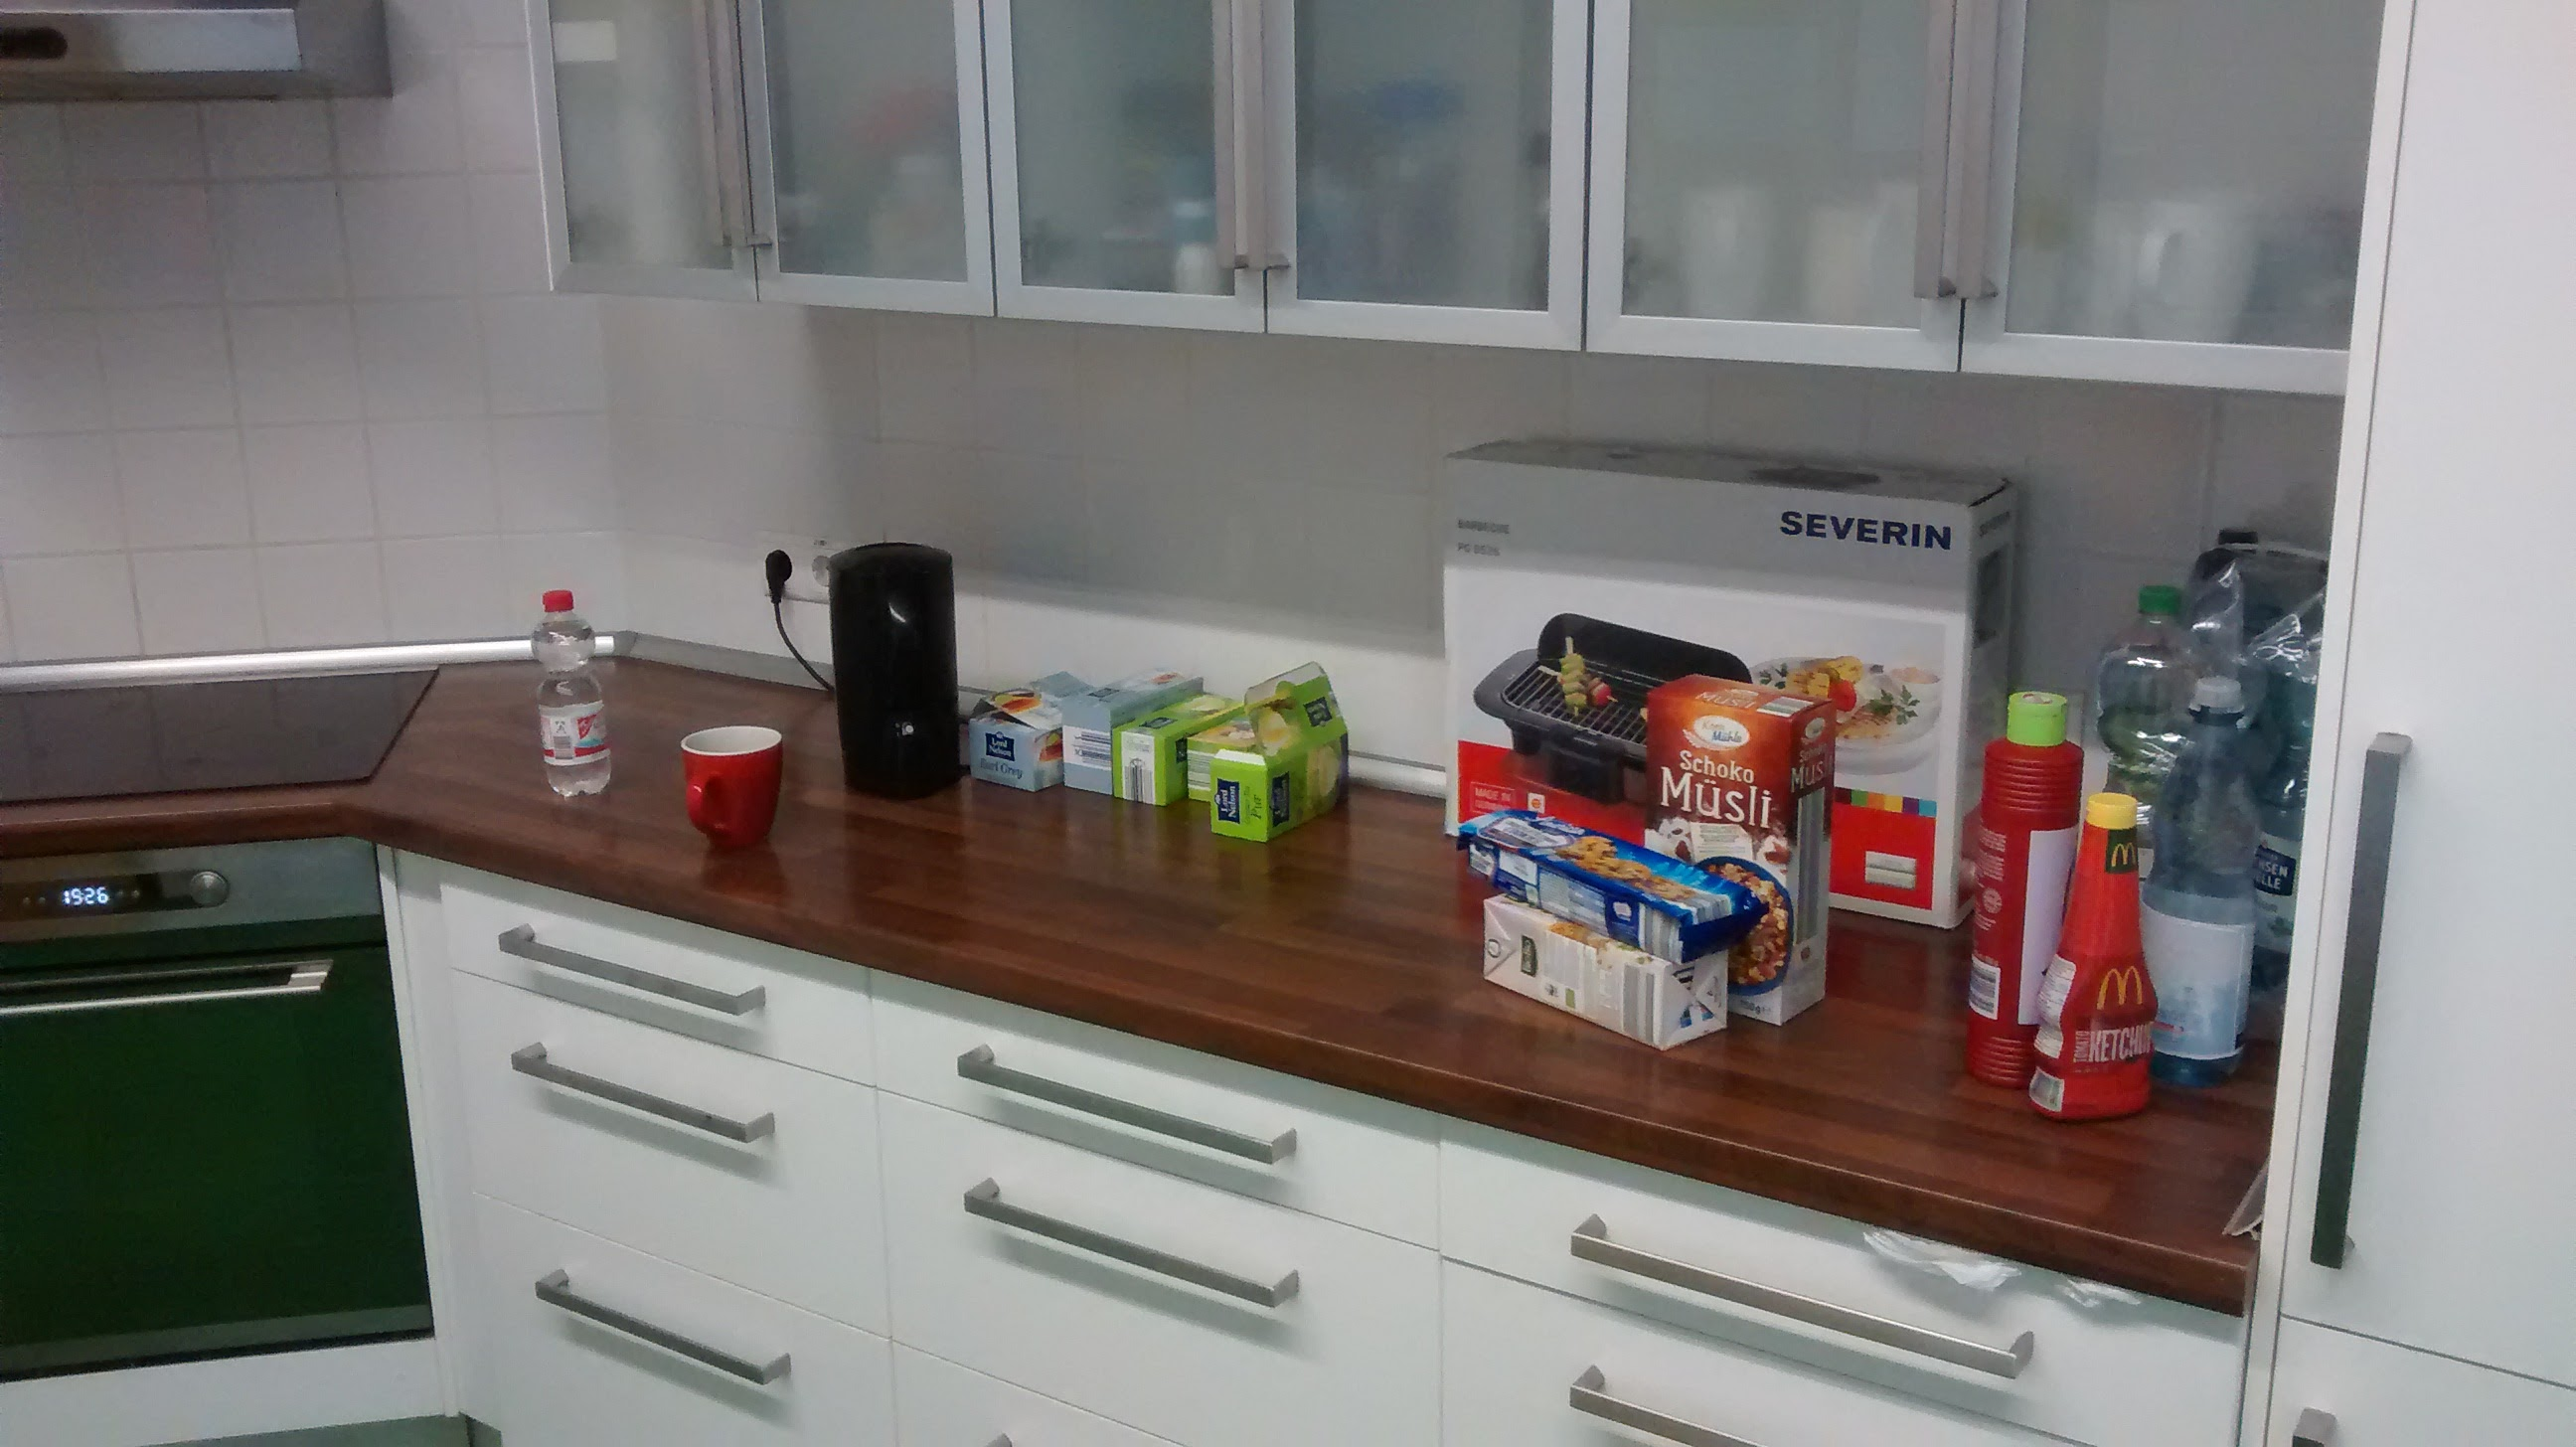
\includegraphics[width=\textwidth]{images/counter-top.jpg}
        \caption{counter-top}
        \label{fig:counter-top}
    \end{subfigure}
    \caption{Different possible object locations}\label{fig:alllocations}
\end{figure}absent_groundtruth.tex}
\end{document}

